% ==============================================================================
% SECCION III: METODOLOGIA
% ==============================================================================
\section{Metodología}\label{sec:metodologia}

Esta sección detalla de forma reproducible el diseño mecánico para fabricación aditiva, la instrumentación electrónica, el protocolo experimental y los métodos de análisis, la arquitectura de firmware en cinco capas con diagramas de bloques atómicos por estado y el gemelo digital~3D en MATLAB. Para cada componente físico, filtro y ley de control se especifican: \textit{(i)}~la necesidad que suple, \textit{(ii)}~el criterio técnico de elección, \textit{(iii)}~su diseño paramétrico o función de transferencia discreta en~$z$ y \textit{(iv)}~su implementación concreta en hardware o código~C. Los fundamentos teóricos y las derivaciones continuas de la planta se omiten por brevedad y se referencian desde la Sección~\ref{sec:marco_teorico}.

\subsection{Diseño Mecánico DfAM y Materiales}\label{subsec:dfam}

La estructura física del péndulo de Furuta se modeló paramétricamente en \texttt{FreeCAD~1.1} aplicando criterios de diseño para fabricación aditiva (DfAM) con cero material de soporte ($\text{SUP}=0$). Frente a un primer diseño monolítico que requería $1\,365$ segmentos de soporte, generaba tres colisiones de montaje ($\qty{0.44}{}$ a $\qty{1.06}{\cubic\milli\meter}$) y demandaba más de \qty{10}{\hour} de tirada continua en una sola torre, se adoptó una arquitectura modular en cuatro subconjuntos ensamblados con tornillería estándar M5/M3/M2 (Fig.~\ref{fig:cad_composicion}), manufacturada en ácido poliláctico (PLA de \qty{1.75}{\milli\meter}) sobre una impresora Anycubic Kobra~2 (cama de $220\times 220\times\qty{250}{\milli\meter}$, extrusor \textit{Direct Drive}, boquilla de \qty{0.4}{\milli\meter}, cama a \qty{60}{\celsius} y boquilla a \qty{210}{\celsius} en primera capa / \qty{205}{\celsius} en régimen; laminado en UltiMaker Cura~5.14+). La Fig.~\ref{fig:cad_composicion} presenta sucesivamente: (a)~el ensamble mecánico completo, (b)~el corte de la torre mostrando el motor Namiki~22CL y el encoder AS5600 base, (c)~la articulación distal con rodamiento \texttt{608ZZ} y (d)~el despiece modular de los componentes impresos.

\begin{figure*}[!t]
    \centering
    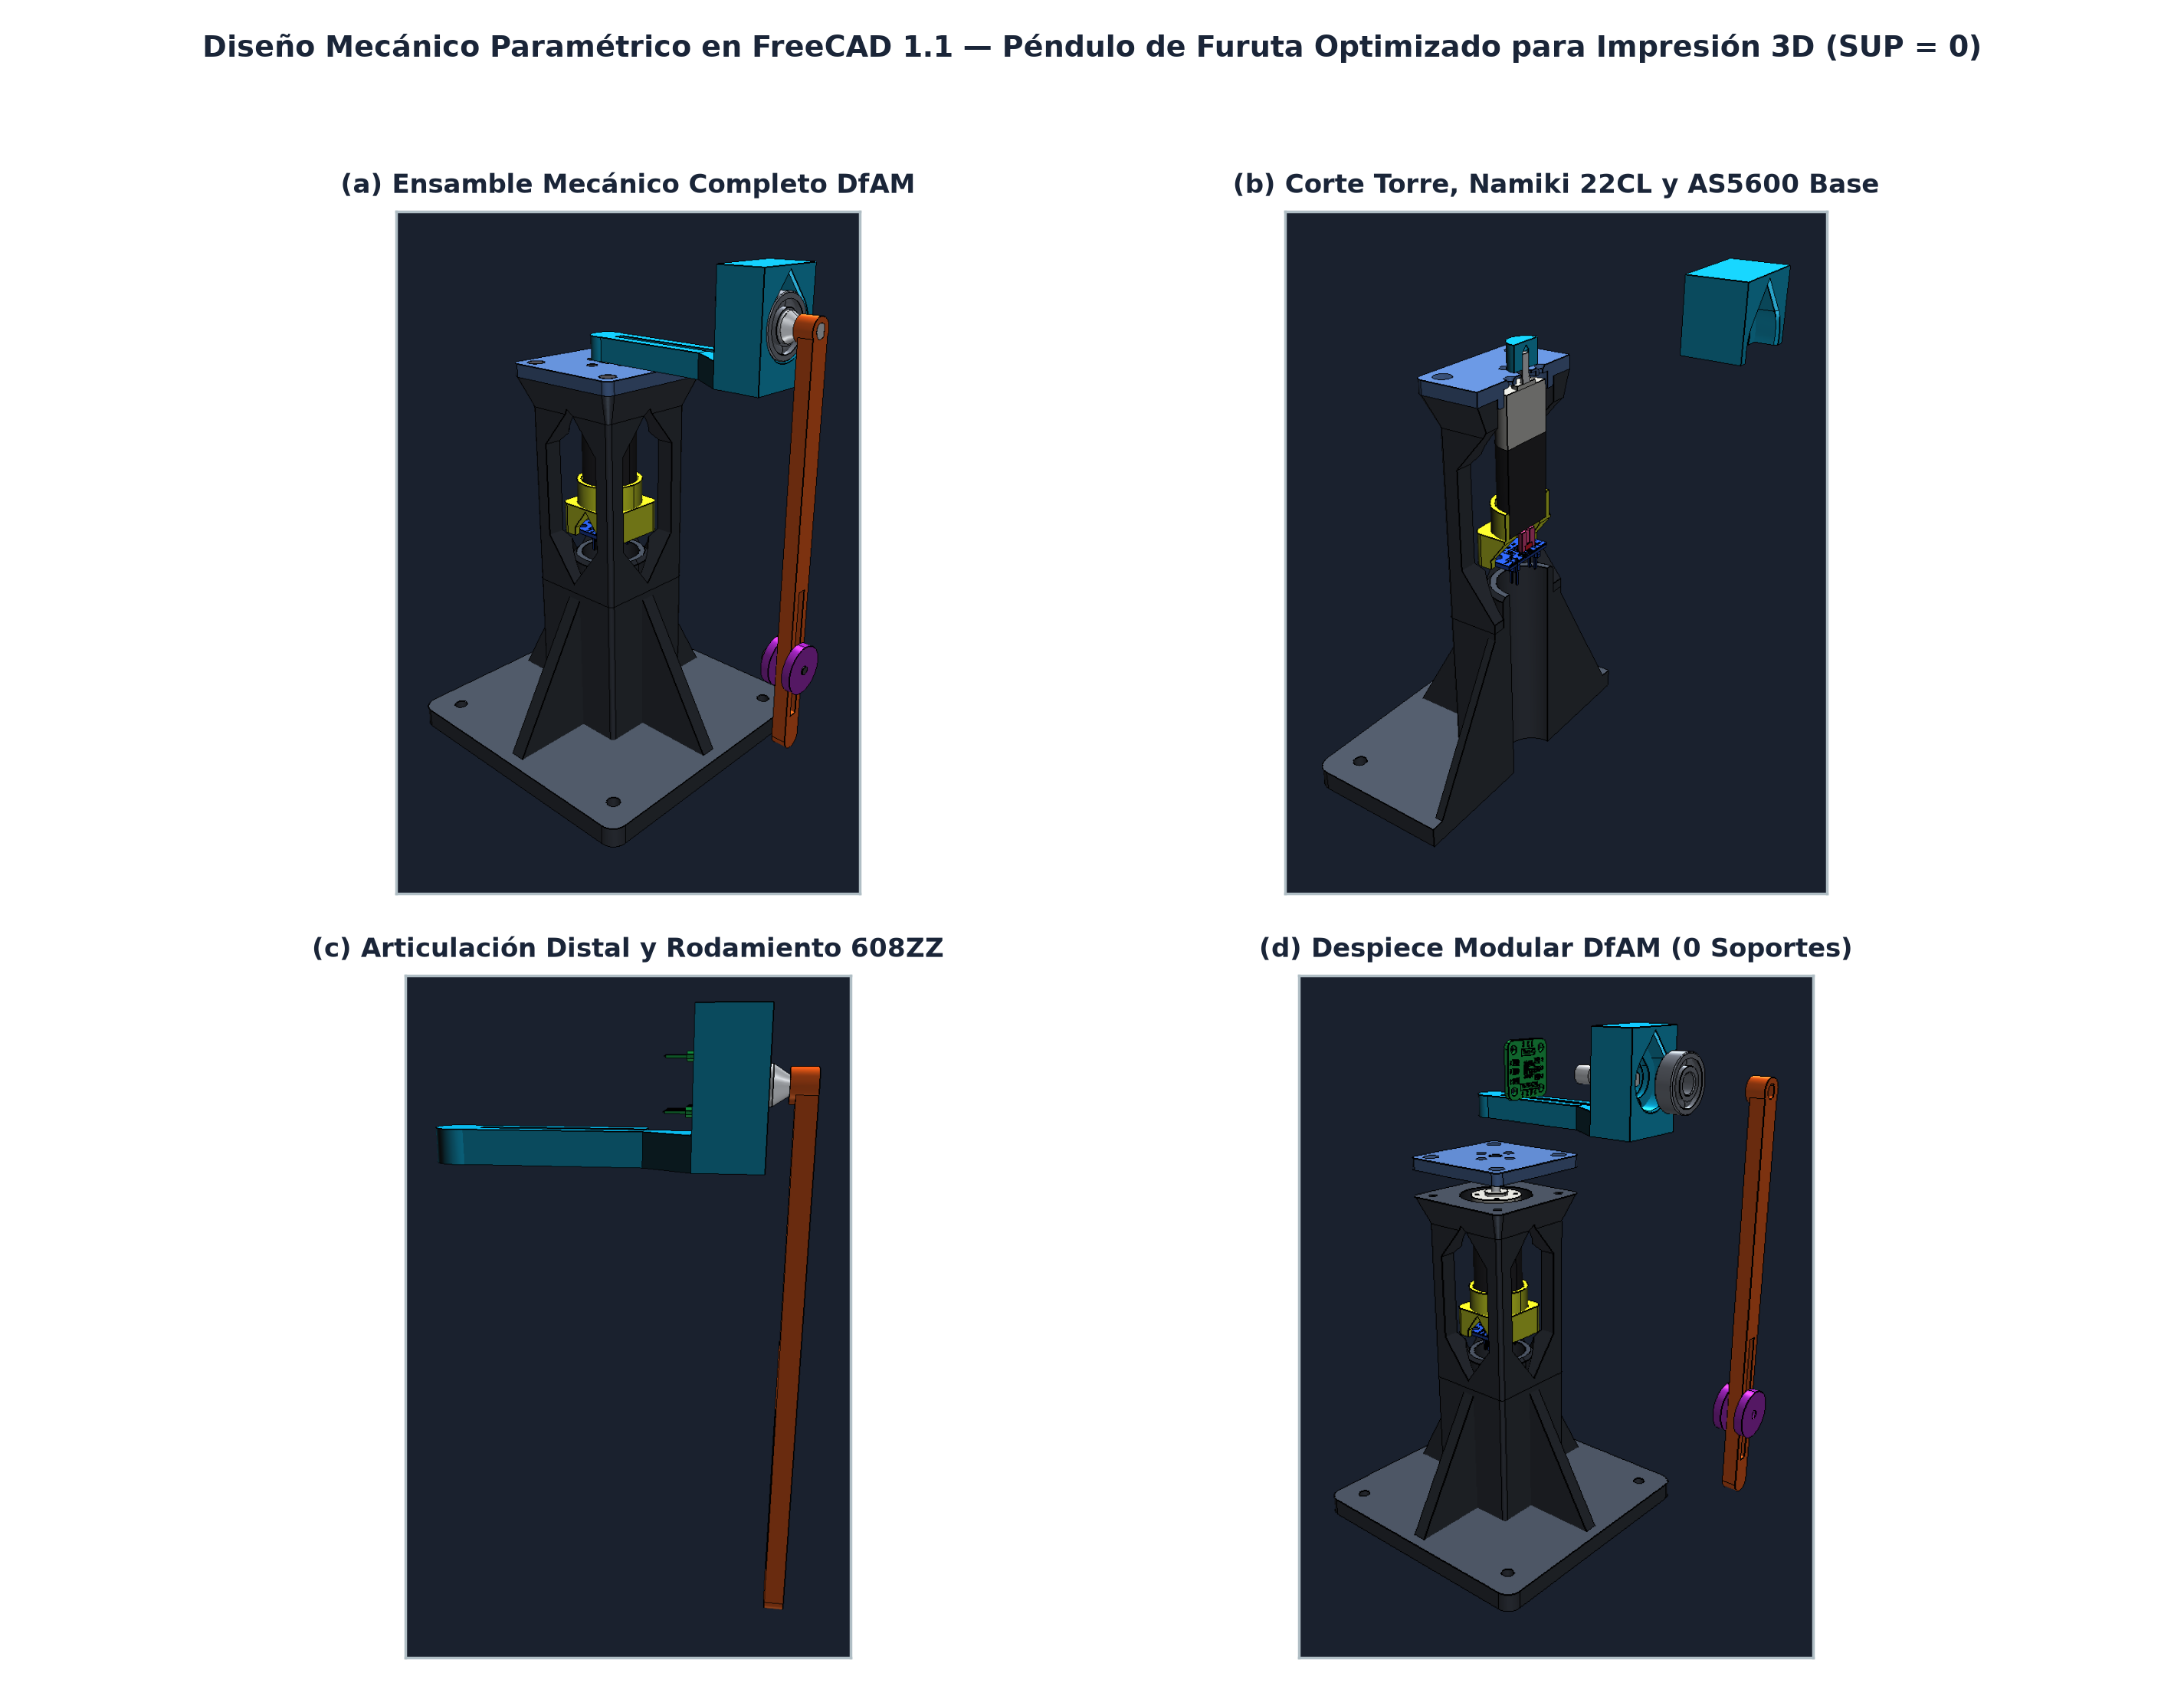
\includegraphics[width=0.90\textwidth]{fig_cad_composicion_mecanica.png}
    \caption{Composición mecánica paramétrica y despiece modular del prototipo.}
    \label{fig:cad_composicion}
\end{figure*}

\begin{enumerate}
    \item \textbf{Base y torre dividida ($H=\qty{160}{\milli\meter}$):}
    \textit{(i)~Necesidad:} elevar el plano de giro por encima de la longitud pendular, absorber los pares torsores de arranque, proteger el motor y permitir acceso manual al cableado.
    \textit{(ii)~Elección:} particionar la torre coaxialmente en el plano $Z=\qty{70}{\milli\meter}$ elimina los puentes horizontales extensos del diseño monolítico y reduce el riesgo de fallo de impresión en placas independientes.
    \textit{(iii)~Diseño:} la base ($120\times\qty{120}{\milli\meter}$, espesor \qty{8}{\milli\meter}, cuatro taladros M5) integra cuatro aletas triangulares de refuerzo ($Z=8\text{--}\qty{68}{\milli\meter}$, $29.5^\circ$ respecto a la vertical), espiga macho coaxial ($\varnothing\qty{31.6}{\milli\meter}\times\qty{12}{\milli\meter}$ con chaflán guía a \qty{45}{\degree}) y barreno central pasante de $\varnothing\qty{24.0}{\milli\meter}$ para los arneses. La torre superior ($Z=70\text{--}\qty{156}{\milli\meter}$) presenta barreno hembra de $\varnothing\qty{32.0}{\milli\meter}$ y cuatro ventanas laterales con doble arco ojival autoportante a $37.8^\circ$ (inferior) y $40.3^\circ$ (superior), ensanchándose en una brida superior de $52\times\qty{52}{\milli\meter}$ cerrada por una tapa desmontable de \qty{5.0}{\milli\meter} (con faldón de \qty{3.5}{\milli\meter} y taladros avellanados M2 rotados \qty{45}{\degree} hacia los ejes cardinales para dirigir el cableado por las ventanas).
    \textit{(iv)~Implementación:} la base se imprimió plana en la placa~P1 (\qty{0.20}{\milli\meter} de capa, $25\%$ Gyroid, 4 paredes); la torre superior se imprimió invertida («boca abajo» sobre su brida de $52\times\qty{52}{\milli\meter}$, logrando $\qty{18.9}{\square\centi\meter}$ de adherencia sin alabeo) en P2, y la tapa en P3, uniéndose mediante cuatro tornillos $\text{M3}\times\qty{12}{\milli\meter}$ accesibles por los vanos laterales.

    \item \textbf{Brazo horizontal monolítico ($L_0=\qty{88.5}{\milli\meter}$):}
    \textit{(i)~Necesidad:} transmitir el par motriz hasta el pivote distal con alta rigidez flexional, sostener el PCB del encoder distal y canalizar sus cuatro hilos sin roce contra la torre.
    \textit{(ii)~Elección:} una viga monolítica con cara inferior coplanar elimina los escalones colgantes de diseños previos y maximiza la resistencia mecánica a flexión en el plano XY sin soportes.
    \textit{(iii)~Diseño:} base continua situada en $Z=\qty{163}{\milli\meter}$ ($\qty{3.0}{\milli\meter}$ de despeje axial anti-roce sobre la torre de $H=\qty{160}{\milli\meter}$), cubo hembra en~D para el eje motor ($\varnothing\qty{4.0}{\milli\meter}$) con techo cónico interno a $39^\circ$, canaleta superior abierta (\texttt{wire\_groove}, $3.6\times\qty{3.0}{\milli\meter}$) y cajera rasante para el PCB AS5600 con pendiente superior de $40^\circ$.
    \textit{(iv)~Implementación:} impreso horizontalmente sobre la cama en P3 (\qty{0.16}{\milli\meter}, $45\%$ Gyroid, 5 paredes) con la cara posterior abierta para atornillar el PCB mediante cuatro tornillos M3.

    \item \textbf{Articulación distal (\texttt{608ZZ} y portaimán sin tornillos):}
    \textit{(i)~Necesidad:} garantizar rotación pendular de mínima fricción con alineación coaxial exacta frente al imán diametral sin holguras ni desbalanceo por prisioneros radiales.
    \textit{(ii)~Elección:} sustituir barrenos cilíndricos horizontales por perfiles en lágrima autoportantes y reemplazar tornillos de fijación por un acople eje--barra en~D con porta-imán coaxial.
    \textit{(iii)~Diseño:} alojamiento con perfil en lágrima (techo ojival a $41^\circ$) calibrado a $\varnothing\qty{22.20}{\milli\meter}$ para compensar la contracción térmica del PLA e insertar manualmente el rodamiento \texttt{608ZZ} ($22\times 8\times\qty{7}{\milli\meter}$), chaflán guía a \qty{45}{\degree}, hombro de apoyo exclusivo sobre la pista exterior ($\varnothing\qty{14.0}{\milli\meter}$) y dos ranuras traseras de expulsión; el eje portaimán integra cono de transición ($32.7^\circ\text{--}41.2^\circ$), rampa en~D a $40.6^\circ$, cuello $\varnothing\qty{7.96}{\milli\meter}$ y copa frontal para el imán diametral con entrehierro nominal de $\sim\qty{0.8}{\milli\meter}$ frente al sensor distal.
    \textit{(iv)~Implementación:} el eje portaimán, el acoplador trasero del motor (unido con cianoacrilato capilar de $\qty{0.08}{\milli\meter}$ de holgura radial) y el portaimán del rotor se imprimieron verticalmente en P4 a \qty{0.12}{\milli\meter} con relleno sólido del $100\%$ (6 paredes) para asegurar concentricidad.

    \item \textbf{Barra pendular ($L_1=\qty{155}{\milli\meter}$):}
    \textit{(i)~Necesidad:} materializar la inercia pendular permitiendo ajustar el centro de masa $l_1$ y completar giros de \qty{360}{\degree} sin colisionar contra la mesa de trabajo.
    \textit{(ii)~Elección:} varilla de cara coplanar con corredera pasante y contrapeso bipartito sujeto por un único tornillo M3, eliminando soportes y concentraciones asimétricas de masa.
    \textit{(iii)~Diseño:} sección rectangular de $8.0\times\qty{5.5}{\milli\meter}$ con cubo en~D pasante sin tornillos parásitos, ranura longitudinal de \qty{50}{\milli\meter} para el contrapeso cilíndrico ($\varnothing\qty{18}{\milli\meter}$) y pivote en $Z_{\text{piv}}=\qty{182.8}{\milli\meter}$ (\qty{152.8}{\milli\meter} pivote--punta redondeada), asegurando exactamente \qty{30}{\milli\meter} de despeje libre sobre el plano mesa ($Z=0$).
    \textit{(iv)~Implementación:} impresa plana en P3 junto con el brazo y la tapa.
\end{enumerate}

Las verificaciones booleanas automatizadas en \texttt{freecad-py} confirmaron cero interferencias volumétricas tanto en el ensamble completo ($0/23$ pares, $\qty{0.0000}{\cubic\milli\meter}$) como en el subconjunto motor--encoder ($0/6$ pares). La Tabla~\ref{tab:placas_impresion} consolida los parámetros y consumos de laminado de las cuatro placas del péndulo ($\text{SUP}=0$ en todas ellas).

\begin{table}[!t]
    \centering
    \caption{Placas de impresión 3D DfAM en Anycubic Kobra~2 (PLA \qty{1.75}{\milli\meter}, boquilla \qty{0.4}{\milli\meter}).}
    \label{tab:placas_impresion}
    \scriptsize
    \setlength{\tabcolsep}{2.6pt}
    \begin{tabular}{@{}llccc@{}}
        \toprule
        \textbf{Placa} & \textbf{Componentes} & \textbf{Tiempo} & \textbf{Masa} & \textbf{Sop.} \\
        \midrule
        P1 & \texttt{Base\_Inferior\_Torre} & 8h 14m & \qty{107.66}{\gram} & $\text{SUP}=0$ \\
        P2 & \texttt{Torre\_Superior\_Motor} & 2h 56m & \qty{34.45}{\gram} & $\text{SUP}=0$ \\
        P3 & \texttt{Brazo\_L88, Barra, Tapa} & 2h 46m & \qty{27.42}{\gram} & $\text{SUP}=0$ \\
        P4 & \texttt{Acoplador, Eje, Portaimán} & 1h 14m & \qty{8.60}{\gram} & $\text{SUP}=0$ \\
        \midrule
        \textbf{P1--P4} & \textbf{Total péndulo de Furuta} & \textbf{15h 10m} & \textbf{\qty{178.13}{\gram}} & \textbf{0} \\
        \bottomrule
    \end{tabular}\par
    \vspace{2pt}
    \raggedright\scriptsize\textit{Nota:} Filamento acumulado P1--P4: \qty{59.72}{\meter} (tiempo exacto de laminado: 15h 09m 44s; $\text{SUP}=0$ en todas las placas).
\end{table}

\subsection{Componentes Electrónicos e Instrumentación Embebida}\label{subsec:electronica}

La arquitectura electrónica integra el microcontrolador, la etapa de potencia de \qty{12}{\volt} con puente~H L298N, el doble bus Soft-$\text{I}^2\text{C}$ con resistencias \textit{pull-up} $R_{\text{pu}}$ hacia ambos encoders AS5600 (acoplado mecánicamente $80:1$ en la base), la interfaz local (\texttt{B1}, \texttt{LD2}) y el enlace \texttt{UART} hacia MATLAB mediante 12 puentes directos 1-a-1 sobre los conectores Arduino de la placa Nucleo sin emplear protoboard (Fig.~\ref{fig:esquematico_electronico} y Tabla~\ref{tab:pinout_stm32}; en el esquemático los trazos distinguen potencia en rojo, PWM \texttt{PA8} en naranja, dirección \texttt{PB4}/\texttt{PB5} en azul, masa común en negro, \texttt{3.3\,V} en carmesí y buses \texttt{SCL}/\texttt{SDA} en verde). A continuación se describe cada subsistema bajo los cuatro pilares de diseño.

% ==============================================================================
% Figura: Esquemático Electrónico e Interconexión Esencial
% Sistema: Péndulo Invertido Rotacional de Furuta (STM32 Nucleo-F446RE)
% Construido por restricciones geométricas relativas (positioning, calc, fit)
% ==============================================================================
\begin{figure*}[!t]
\centering
% Paleta técnica local
\definecolor{mcuBorder}{HTML}{1B3A6B}
\definecolor{mcuFill}{HTML}{F2F6FC}
\definecolor{mcuHead}{HTML}{1B3A6B}
\definecolor{pwrBorder}{HTML}{9E2A2B}
\definecolor{pwrFill}{HTML}{FDF4F4}
\definecolor{pwrHead}{HTML}{9E2A2B}
\definecolor{motBorder}{HTML}{B45309}
\definecolor{motFill}{HTML}{FFFBF0}
\definecolor{motHead}{HTML}{B45309}
\definecolor{senBorder}{HTML}{0F766E}
\definecolor{senFill}{HTML}{F0FDFA}
\definecolor{senHead}{HTML}{0F766E}
\definecolor{telBorder}{HTML}{3730A3}
\definecolor{telFill}{HTML}{F1F3FF}
\definecolor{telHead}{HTML}{3730A3}
\definecolor{wirePwr}{HTML}{B91C1C}
\definecolor{wireVcc}{HTML}{DC2626}
\definecolor{wireGnd}{HTML}{1F2937}
\definecolor{wirePwm}{HTML}{C2410C}
\definecolor{wireGpio}{HTML}{1D4ED8}
\definecolor{wireScl}{HTML}{0F766E}
\definecolor{wireSda}{HTML}{15803D}
\definecolor{wireUart}{HTML}{3730A3}
\definecolor{wireMech}{HTML}{78350F}
%
\resizebox{0.94\textwidth}{!}{%
\begin{circuitikz}[
    >=Stealth,
    font=\sffamily,
    % --- Parámetros de ritmo geométrico (fuente única de verdad) ---
    /tikz/hdrnode/.style={
        rectangle,
        minimum width=#1,
        text width=\dimexpr #1 - 14pt\relax,
        align=center,
        text=white,
        font=\normalsize\bfseries,
        inner xsep=7pt,
        inner ysep=6pt
    },
    pinlbl/.style={font=\small\ttfamily\bfseries, inner sep=1pt},
    wirelbl/.style={font=\small\sffamily\bfseries, inner sep=1.5pt},
    bushead/.style={
        font=\footnotesize\sffamily\bfseries, fill=white,
        draw=#1!65, text=#1, rounded corners=2pt, inner xsep=5pt, inner ysep=2pt
    },
    pinport/.style={circle, fill=white, draw=black!80, line width=0.75pt, inner sep=1.5pt},
    solder/.style={circle, fill=black!85, inner sep=1.5pt}
]
% Dimensiones paramétricas globales
\def\mcuW{7.0cm}
\def\leftW{3.7cm}
\def\senW{3.4cm}
\def\uiW{3.5cm}
\def\pcW{3.4cm}
\def\gapLeft{3.4cm}
\def\gapRight{4.2cm}
\def\rowGap{1.00cm}
\def\pinPitch{0.78cm}
\def\botGap{1.05cm}
\def\botH{2.15cm}

% ==============================================================================
% 1. NODO RAÍZ: ENCABEZADO STM32 NUCLEO-F446RE
% ==============================================================================
\node[hdrnode=\mcuW, anchor=north] (mcu_hdr) at (0,0) {STM32 Nucleo-F446RE};

% ==============================================================================
% 2. COLUMNA DERECHA: SENSORES AS5600 BASE (I2C1) Y DISTAL (I2C2)
% ==============================================================================
\node[hdrnode=\senW, right=\gapRight of mcu_hdr.north east, anchor=north west] (as1_hdr) {AS5600 Base};

\coordinate (as1_scl) at ($(as1_hdr.south west)+(0,-0.68cm)$);
\coordinate (as1_vcc) at ($(as1_scl)+(0,-\pinPitch)$);
\coordinate (as1_sda) at ($(as1_vcc)+(0,-\pinPitch)$);
\coordinate (as1_gnd) at ($(as1_sda)+(0,-\pinPitch)$);
\coordinate (as1_bot) at ($(as1_gnd)+(0,-0.46cm)$);
\node[draw=none, fill=none, inner sep=0pt, fit=(as1_hdr)(as1_bot)] (as1) {};

\node[pinlbl, anchor=west, text=wireScl] at ($(as1_scl)+(6pt,0)$) {SCL};
\node[pinlbl, anchor=west, text=wireVcc] at ($(as1_vcc)+(6pt,0)$) {VCC};
\node[pinlbl, anchor=west, text=wireSda] at ($(as1_sda)+(6pt,0)$) {SDA};
\node[pinlbl, anchor=west, text=wireGnd] at ($(as1_gnd)+(6pt,0)$) {GND};

% Sensor 2 debajo de Sensor 1
\node[hdrnode=\senW, below=\rowGap of as1.south west, anchor=north west] (as2_hdr) {AS5600 Distal};

\coordinate (as2_scl) at ($(as2_hdr.south west)+(0,-0.68cm)$);
\coordinate (as2_vcc) at ($(as2_scl)+(0,-\pinPitch)$);
\coordinate (as2_sda) at ($(as2_vcc)+(0,-\pinPitch)$);
\coordinate (as2_gnd) at ($(as2_sda)+(0,-\pinPitch)$);
\coordinate (as2_bot) at ($(as2_gnd)+(0,-0.46cm)$);
\node[draw=none, fill=none, inner sep=0pt, fit=(as2_hdr)(as2_bot)] (as2) {};

\node[pinlbl, anchor=west, text=wireScl] at ($(as2_scl)+(6pt,0)$) {SCL};
\node[pinlbl, anchor=west, text=wireVcc] at ($(as2_vcc)+(6pt,0)$) {VCC};
\node[pinlbl, anchor=west, text=wireSda] at ($(as2_sda)+(6pt,0)$) {SDA};
\node[pinlbl, anchor=west, text=wireGnd] at ($(as2_gnd)+(6pt,0)$) {GND};

% ==============================================================================
% 3. COLUMNA IZQUIERDA: MOTOR DC, DRIVER L298N Y FUENTE 12 V
% ==============================================================================
\node[hdrnode=\leftW, left=\gapLeft of mcu_hdr.north west, anchor=north east] (motor_hdr) {Motor DC};

\node[elmech, scale=0.68, fill=white, draw=motBorder, line width=1.0pt,
      below=0.38cm of motor_hdr.south] (m_sym) {M};
\coordinate (motor_bot) at ($(m_sym.south)+(0,-0.46cm)$);
\node[draw=none, fill=none, inner sep=0pt, fit=(motor_hdr)(motor_bot)] (motor) {};

\node[font=\small\bfseries, text=motHead, anchor=south east] at ($(m_sym.left)+(-3pt,2pt)$) {$+$};
\node[font=\small\bfseries, text=motHead, anchor=south west] at ($(m_sym.right)+(3pt,2pt)$) {$-$};

\coordinate (mot_out1) at ($(motor.south west)!0.26!(motor.south east)$);
\coordinate (mot_out2) at ($(motor.south west)!0.74!(motor.south east)$);
\draw[motBorder, line width=1.05pt] (m_sym.left)  -| (mot_out1);
\draw[motBorder, line width=1.05pt] (m_sym.right) -| (mot_out2);

% Driver L298N
\node[hdrnode=\leftW, below=\rowGap of motor.south west, anchor=north west] (l298_hdr) {Driver L298N};

\coordinate (l298_ena) at ($(l298_hdr.south east)+(0,-0.56cm)$);
\coordinate (l298_in1) at ($(l298_ena)+(0,-\pinPitch)$);
\coordinate (l298_in2) at ($(l298_in1)+(0,-\pinPitch)$);
\coordinate (l298_gnd) at ($(l298_in2)+(0,-\pinPitch)$);
\coordinate (l298_bot) at ($(l298_gnd)+(0,-0.64cm)$);
\node[draw=none, fill=none, inner sep=0pt, fit=(l298_hdr)(l298_bot)] (l298n) {};

\coordinate (l298_out1) at (l298n.north -| mot_out1);
\coordinate (l298_out2) at (l298n.north -| mot_out2);
\draw[wirePwr, line width=1.35pt, ->] (l298_out1) -- (mot_out1);
\draw[wirePwr, line width=1.35pt, ->] (l298_out2) -- (mot_out2);
\node[wirelbl, text=wirePwr, anchor=east] at ($(l298_out1)!0.5!(mot_out1)+(-4pt,0)$) {OUT1};
\node[wirelbl, text=wirePwr, anchor=west] at ($(l298_out2)!0.5!(mot_out2)+( 4pt,0)$) {OUT2};

\node[pinlbl, anchor=east, text=wirePwm]  at ($(l298_ena)+(-6pt,0)$) {ENA};
\node[pinlbl, anchor=east, text=wireGpio] at ($(l298_in1)+(-6pt,0)$) {IN1};
\node[pinlbl, anchor=east, text=wireGpio] at ($(l298_in2)+(-6pt,0)$) {IN2};
\node[pinlbl, anchor=east, text=wireGnd]  at ($(l298_gnd)+(-6pt,0)$) {GND};

\coordinate (l298_vms)  at ($(l298n.south west)!0.18!(l298n.south east)$);
\coordinate (l298_pgnd) at ($(l298n.south west)!0.84!(l298n.south east)$);
\node[pinlbl, text=wirePwr, anchor=south] at ($(l298_vms)+(0,4pt)$)  {VMS};
\node[pinlbl, text=wireGnd, anchor=south] at ($(l298_pgnd)+(0,4pt)$) {GND};

% Fuente 12 V
\coordinate (psu_nw)      at ($(l298n.south west)+(0,-1.10cm)$);
\coordinate (psu_ne)      at ($(l298n.south east)+(0,-1.10cm)$);
\coordinate (psu_in_vms)  at (l298_vms |- psu_nw);
\coordinate (psu_in_gnd)  at (l298_pgnd |- psu_nw);
\coordinate (psu_src_top) at ($(psu_in_vms)+(0,-0.40cm)$);
\coordinate (psu_src_bot) at ($(psu_src_top)+(0,-1.65cm)$);
\coordinate (psu_gnd_cor) at (psu_in_gnd |- psu_src_bot);
\coordinate (psu_ne_bot)  at (psu_ne |- psu_src_bot);
\coordinate (psu_se)      at ($(psu_ne_bot)+(0,-0.40cm)$);
\node[draw=none, fill=none, inner sep=0pt, fit=(psu_nw)(psu_se)] (psu) {};

\draw[wirePwr, line width=1.35pt] (l298_vms) -- (psu_in_vms);
\node[wirelbl, text=wirePwr, anchor=east]
    at ($(l298_vms)!0.50!(psu_in_vms)+(-4pt,0)$) {+\qty{12}{\volt}};

\draw[wirePwr, line width=1.15pt] (psu_in_vms) -- (psu_src_top);
\draw[wirePwr, line width=1.15pt] (psu_src_top) to[vsource, american] (psu_src_bot);
\draw[wireGnd, line width=1.20pt]
    (psu_src_bot) -- (psu_gnd_cor) -- (psu_in_gnd) -- (l298_pgnd);

\coordinate (psu_lbl_x) at ($(psu_in_vms)!0.54!(psu_in_gnd)$);
\coordinate (psu_lbl_y) at ($(psu_src_top)!0.50!(psu_src_bot)$);
\node[font=\normalsize\bfseries, text=pwrHead, align=center]
    at (psu_lbl_x |- psu_lbl_y) {Fuente\\\qty{12}{\volt}};

% ==============================================================================
% 4. CAJA MCU CENTRAL Y PINES ORTOGONALES
% ==============================================================================
\coordinate (mcu_bot_y)   at ($(as2.south)+(0,-0.25cm)$);
\coordinate (mcu_bot_ref) at (mcu_hdr.south |- mcu_bot_y);
\node[draw=none, fill=none, inner sep=0pt, fit=(mcu_hdr)(mcu_bot_ref)] (mcu) {};

% Proyecciones de pines hacia bordes de MCU
\coordinate (mcu_scl1)  at (mcu.east |- as1_scl);
\coordinate (mcu_3v3)   at (mcu.east |- as1_vcc);
\coordinate (mcu_sda1)  at (mcu.east |- as1_sda);
\coordinate (mcu_gnd1)  at (mcu.east |- as1_gnd);

\coordinate (mcu_scl2)  at (mcu.east |- as2_scl);
\coordinate (mcu_ioref) at (mcu.east |- as2_vcc);
\coordinate (mcu_sda2)  at (mcu.east |- as2_sda);
\coordinate (mcu_gnd2)  at (mcu.east |- as2_gnd);

\coordinate (mcu_ena)   at (mcu.west |- l298_ena);
\coordinate (mcu_in1)   at (mcu.west |- l298_in1);
\coordinate (mcu_in2)   at (mcu.west |- l298_in2);
\coordinate (mcu_gnd0)  at (mcu.west |- l298_gnd);

% Pines MCU derecha
\node[pinlbl, anchor=east, text=wireScl] at ($(mcu_scl1)+(-6pt,0)$)  {PB8};
\node[pinlbl, anchor=east, text=wireVcc] at ($(mcu_3v3)+(-6pt,0)$)   {3V3};
\node[pinlbl, anchor=east, text=wireSda] at ($(mcu_sda1)+(-6pt,0)$)  {PB9};
\node[pinlbl, anchor=east, text=wireGnd] at ($(mcu_gnd1)+(-6pt,0)$)  {GND};

\node[pinlbl, anchor=east, text=wireScl] at ($(mcu_scl2)+(-6pt,0)$)  {PB10};
\node[pinlbl, anchor=east, text=wireVcc] at ($(mcu_ioref)+(-6pt,0)$) {IOREF};
\node[pinlbl, anchor=east, text=wireSda] at ($(mcu_sda2)+(-6pt,0)$)  {PB3};
\node[pinlbl, anchor=east, text=wireGnd] at ($(mcu_gnd2)+(-6pt,0)$)  {GND};

% Pines MCU izquierda
\node[pinlbl, anchor=west, text=wirePwm]  at ($(mcu_ena)+(6pt,0)$)  {PA8};
\node[pinlbl, anchor=west, text=wireGpio] at ($(mcu_in1)+(6pt,0)$)  {PB4};
\node[pinlbl, anchor=west, text=wireGpio] at ($(mcu_in2)+(6pt,0)$)  {PB5};
\node[pinlbl, anchor=west, text=wireGnd]  at ($(mcu_gnd0)+(6pt,0)$) {GND};

% ==============================================================================
% 5. BUSES DERECHOS (I2C1, I2C2) Y BUSES IZQUIERDOS (PWM/GPIO/MASA COMÚN)
% ==============================================================================
\node[bushead=senBorder, anchor=south] at ($(mcu_scl1)!0.52!(as1_scl)+(0,0.34cm)$)
    {$\text{I}^2\text{C}_1$};
\node[bushead=senBorder, anchor=south] at ($(mcu_scl2)!0.52!(as2_scl)+(0,0.34cm)$)
    {$\text{I}^2\text{C}_2$};

% Bus I2C1
\draw[wireScl, line width=1.10pt, ->]   (mcu_scl1) -- (as1_scl);
\draw[wireVcc, line width=1.15pt]       (mcu_3v3)  -- (as1_vcc);
\draw[wireSda, line width=1.10pt, <->]  (mcu_sda1) -- (as1_sda);
\draw[wireGnd, line width=1.15pt]       (mcu_gnd1) -- (as1_gnd);

\node[wirelbl, text=wireScl, above=2pt] at ($(mcu_scl1)!0.20!(as1_scl)$) {SCL1};
\node[wirelbl, text=wireVcc, above=2pt] at ($(mcu_3v3)!0.20!(as1_vcc)$)  {\qty{3.3}{\volt}};
\node[wirelbl, text=wireSda, above=2pt] at ($(mcu_sda1)!0.20!(as1_sda)$) {SDA1};
\node[wirelbl, text=wireGnd, above=2pt] at ($(mcu_gnd1)!0.20!(as1_gnd)$) {GND};

% Pull-ups I2C1
\coordinate (pu1_scl_t) at ($(mcu_scl1)!0.54!(as1_scl)$);
\coordinate (pu1_scl_b) at ($(mcu_3v3)!0.54!(as1_vcc)$);
\coordinate (pu1_sda_t) at ($(mcu_3v3)!0.78!(as1_vcc)$);
\coordinate (pu1_sda_b) at ($(mcu_sda1)!0.78!(as1_sda)$);
\draw[senBorder!85!black, line width=0.80pt]
    (pu1_scl_t) to[R, resistors/scale=0.40] (pu1_scl_b);
\draw[senBorder!85!black, line width=0.80pt]
    (pu1_sda_t) to[R, resistors/scale=0.40] (pu1_sda_b);
\node[solder, fill=wireScl] at (pu1_scl_t) {};
\node[solder, fill=wireVcc] at (pu1_scl_b) {};
\node[solder, fill=wireVcc] at (pu1_sda_t) {};
\node[solder, fill=wireSda] at (pu1_sda_b) {};
\node[font=\footnotesize, text=senHead, anchor=east] at ($(pu1_scl_t)!0.5!(pu1_scl_b)+(-5pt,0)$) {$R_{\text{pu}}$};
\node[font=\footnotesize, text=senHead, anchor=west] at ($(pu1_sda_t)!0.5!(pu1_sda_b)+( 5pt,0)$) {$R_{\text{pu}}$};

% Bus I2C2
\draw[wireScl, line width=1.10pt, ->]   (mcu_scl2)  -- (as2_scl);
\draw[wireVcc, line width=1.15pt]       (mcu_ioref) -- (as2_vcc);
\draw[wireSda, line width=1.10pt, <->]  (mcu_sda2)  -- (as2_sda);
\draw[wireGnd, line width=1.15pt]       (mcu_gnd2)  -- (as2_gnd);

\node[wirelbl, text=wireScl, above=2pt] at ($(mcu_scl2)!0.20!(as2_scl)$)  {SCL2};
\node[wirelbl, text=wireVcc, above=2pt] at ($(mcu_ioref)!0.20!(as2_vcc)$) {\qty{3.3}{\volt}};
\node[wirelbl, text=wireSda, above=2pt] at ($(mcu_sda2)!0.20!(as2_sda)$)  {SDA2};
\node[wirelbl, text=wireGnd, above=2pt] at ($(mcu_gnd2)!0.20!(as2_gnd)$)  {GND};

% Pull-ups I2C2
\coordinate (pu2_scl_t) at ($(mcu_scl2)!0.54!(as2_scl)$);
\coordinate (pu2_scl_b) at ($(mcu_ioref)!0.54!(as2_vcc)$);
\coordinate (pu2_sda_t) at ($(mcu_ioref)!0.78!(as2_vcc)$);
\coordinate (pu2_sda_b) at ($(mcu_sda2)!0.78!(as2_sda)$);
\draw[senBorder!85!black, line width=0.80pt]
    (pu2_scl_t) to[R, resistors/scale=0.40] (pu2_scl_b);
\draw[senBorder!85!black, line width=0.80pt]
    (pu2_sda_t) to[R, resistors/scale=0.40] (pu2_sda_b);
\node[solder, fill=wireScl] at (pu2_scl_t) {};
\node[solder, fill=wireVcc] at (pu2_scl_b) {};
\node[solder, fill=wireVcc] at (pu2_sda_t) {};
\node[solder, fill=wireSda] at (pu2_sda_b) {};
\node[font=\footnotesize, text=senHead, anchor=east] at ($(pu2_scl_t)!0.5!(pu2_scl_b)+(-5pt,0)$) {$R_{\text{pu}}$};
\node[font=\footnotesize, text=senHead, anchor=west] at ($(pu2_sda_t)!0.5!(pu2_sda_b)+( 5pt,0)$) {$R_{\text{pu}}$};

% Buses L298N <-> MCU
\draw[wirePwm,  line width=1.25pt, ->] (mcu_ena)  -- (l298_ena);
\draw[wireGpio, line width=1.10pt, ->] (mcu_in1)  -- (l298_in1);
\draw[wireGpio, line width=1.10pt, ->] (mcu_in2)  -- (l298_in2);
\draw[wireGnd,  line width=1.20pt]     (mcu_gnd0) -- (l298_gnd);

\node[wirelbl, text=wirePwm, above=2pt] at ($(mcu_ena)!0.50!(l298_ena)$)  {PWM};
\node[wirelbl, text=wireGnd, above=2pt] at ($(l298_gnd)!0.72!(mcu_gnd0)$) {GND};

% Masa Común
\coordinate (gnd_star_top) at ($(l298_gnd)!0.38!(mcu_gnd0)$);
\coordinate (gnd_psu_tap)  at ($(l298_pgnd)!0.55!(psu_in_gnd)$);
\coordinate (gnd_star_mid) at (gnd_star_top |- gnd_psu_tap);

\draw[wireGnd, line width=1.20pt] (gnd_star_top) -- (gnd_star_mid) -- (gnd_psu_tap);
\draw[wireGnd, line width=1.20pt] (gnd_star_mid) -- ++(0,-0.62cm) node[ground] (gnd_sym) {};
\node[solder, fill=wireGnd] at (gnd_star_top) {};
\node[solder, fill=wireGnd] at (gnd_psu_tap)  {};
\node[solder, fill=wireGnd] at (gnd_star_mid) {};
\node[font=\footnotesize\bfseries, text=wireGnd, align=center, below=2pt]
    at (gnd_sym.south) {GND común};

% ==============================================================================
% 6. CORREDOR SUPERIOR: ACOPLE MECÁNICO 80:1
% ==============================================================================
\coordinate (mech_start) at (motor.north);
\coordinate (mech_end)   at (as1.north);
\coordinate (mech_top_l) at ($(mech_start)+(0,0.80cm)$);
\coordinate (mech_top_r) at ($(mech_end)+(0,0.80cm)$);

\draw[wireMech, line width=1.35pt, densely dashed, ->, rounded corners=4pt]
    (mech_start) -- (mech_top_l) -- (mech_top_r) -- (mech_end);
\node[
    rectangle, rounded corners=2.5pt,
    draw=wireMech!75, fill=motFill, line width=0.85pt,
    font=\small\bfseries, text=wireMech, inner xsep=8pt, inner ysep=3pt
] at ($(mech_top_l)!0.50!(mech_top_r)$) {Acople 80:1};

% ==============================================================================
% 7. FILA INFERIOR: INTERFAZ NUCLEO (B1, LD2) Y PC (MATLAB)
% ==============================================================================
% Interfaz Nucleo debajo de la mitad izquierda de STM32
\coordinate (uiblk_nw) at ($(mcu.south west)+(0,-\botGap)$);
\node[draw=none, fill=none, minimum width=\uiW, minimum height=\botH,
      inner sep=0pt, anchor=north west] (uiblk) at (uiblk_nw) {};

\node[hdrnode=\uiW, anchor=south west] (uiblk_ftr) at (uiblk.south west) {Interfaz Nucleo};

\coordinate (uiblk_b1_top)  at ($(uiblk.north west)!0.28!(uiblk.north east)$);
\coordinate (uiblk_ld2_top) at ($(uiblk.north west)!0.58!(uiblk.north east)$);

\coordinate (mcu_pc13) at (mcu.south -| uiblk_b1_top);
\coordinate (mcu_pa5)  at (mcu.south -| uiblk_ld2_top);

\node[pinlbl, text=telBorder, anchor=south] at ($(mcu_pc13)+(0,5pt)$) {PC13};
\node[pinlbl, text=telBorder, anchor=south] at ($(mcu_pa5)+(0,5pt)$)  {PA5};

\coordinate (b1_s1) at ($(uiblk_b1_top)+(0,-0.24cm)$);
\coordinate (b1_s2) at ($(uiblk_b1_top)+(0,-1.06cm)$);
\draw[telBorder, line width=1.10pt, <-] (mcu_pc13) -- (uiblk_b1_top);
\draw[telBorder, line width=0.95pt]     (uiblk_b1_top) -- (b1_s1)
    to[push button, switches/scale=0.52] (b1_s2) node[ground, scale=0.55] {};
\node[font=\small\bfseries, text=telHead, anchor=east]
    at ($(b1_s1)!0.48!(b1_s2)+(-9pt,0)$) {B1};

\coordinate (ld2_s1) at ($(uiblk_ld2_top)+(0,-0.24cm)$);
\coordinate (ld2_s2) at ($(uiblk_ld2_top)+(0,-1.06cm)$);
\draw[telBorder, line width=1.10pt, ->] (mcu_pa5) -- (uiblk_ld2_top);
\draw[telBorder, line width=0.95pt]     (uiblk_ld2_top) -- (ld2_s1)
    to[leD, diodes/scale=0.50, color=wireSda] (ld2_s2) node[ground, scale=0.55] {};
\node[font=\small\bfseries, text=wireSda, anchor=west]
    at ($(ld2_s1)!0.48!(ld2_s2)+(17pt,0)$) {LD2};

% PC (MATLAB) debajo de AS5600 Distal (alineado en fila inferior)
\coordinate (pc_ne) at (as2.east |- uiblk.north);
\node[draw=none, fill=none, minimum width=\pcW, minimum height=\botH,
      inner sep=0pt, anchor=north east] (pc) at (pc_ne) {};
\node[font=\normalsize\bfseries, text=telHead, align=center] at (pc.center) {PC\\(MATLAB)};

% Conexiones UART PA2 (TX) y PA3 (RX)
\coordinate (mcu_pa3) at ($(mcu.south west)!0.59!(mcu.south east)$);
\coordinate (mcu_pa2) at ($(mcu.south west)!0.87!(mcu.south east)$);
\coordinate (pc_tx_in)  at ($(pc.north west)!0.36!(pc.south west)$);
\coordinate (pc_rx_out) at ($(pc.north west)!0.74!(pc.south west)$);
\coordinate (uart_turn_tx) at (mcu_pa2 |- pc_tx_in);
\coordinate (uart_turn_rx) at (mcu_pa3 |- pc_rx_out);

\node[pinlbl, text=wireUart, anchor=south] at ($(mcu_pa3)+(0,5pt)$) {PA3 (RX)};
\node[pinlbl, text=wireUart, anchor=south] at ($(mcu_pa2)+(0,5pt)$) {PA2 (TX)};

\draw[wireUart, line width=1.15pt, ->, rounded corners=3pt]
    (mcu_pa2) -- (uart_turn_tx) -- (pc_tx_in);
\draw[wireUart, line width=1.15pt, <-, rounded corners=3pt]
    (mcu_pa3) -- (uart_turn_rx) -- (pc_rx_out);

\node[wirelbl, text=wireUart, above=2pt] at ($(uart_turn_tx)!0.50!(pc_tx_in)$) {TX};
\node[wirelbl, text=wireUart, above=2pt] at ($(uart_turn_rx)!0.55!(pc_rx_out)$) {RX};
\node[bushead=telBorder, anchor=south] at ($(uart_turn_tx)!0.50!(pc_tx_in)+(0,0.56cm)$) {UART};

% ==============================================================================
% 8. CAPA DE FONDO Y MARCOS
% ==============================================================================
\begin{scope}[on background layer]
    % MCU
    \path[fill=mcuFill, rounded corners=4pt] (mcu.north west) rectangle (mcu.south east);
    \coordinate (mcu_hb_w) at (mcu.west |- mcu_hdr.south);
    \coordinate (mcu_hb_e) at (mcu.east |- mcu_hdr.south);
    \fill[mcuHead, rounded corners=4pt] (mcu.north west) rectangle (mcu_hb_e);
    \fill[mcuHead] ($(mcu_hb_w)+(0,5pt)$) rectangle (mcu_hb_e);
    \draw[mcuBorder, rounded corners=4pt, line width=1.4pt] (mcu.north west) rectangle (mcu.south east);

    % Sensores AS5600 Base y Distal
    \foreach \s in {as1, as2} {
        \path[fill=senFill, rounded corners=3.5pt] (\s.north west) rectangle (\s.south east);
        \coordinate (\s_hb_w) at (\s.west |- \s_hdr.south);
        \coordinate (\s_hb_e) at (\s.east |- \s_hdr.south);
        \fill[senHead, rounded corners=3.5pt] (\s.north west) rectangle (\s_hb_e);
        \fill[senHead] ($(\s_hb_w)+(0,5pt)$) rectangle (\s_hb_e);
        \draw[senBorder, rounded corners=3.5pt, line width=1.2pt] (\s.north west) rectangle (\s.south east);
    }

    % Motor DC
    \path[fill=motFill, rounded corners=3.5pt] (motor.north west) rectangle (motor.south east);
    \coordinate (mot_hb_w) at (motor.west |- motor_hdr.south);
    \coordinate (mot_hb_e) at (motor.east |- motor_hdr.south);
    \fill[motHead, rounded corners=3.5pt] (motor.north west) rectangle (mot_hb_e);
    \fill[motHead] ($(mot_hb_w)+(0,5pt)$) rectangle (mot_hb_e);
    \draw[motBorder, rounded corners=3.5pt, line width=1.2pt] (motor.north west) rectangle (motor.south east);

    % Driver L298N
    \path[fill=pwrFill, rounded corners=3.5pt] (l298n.north west) rectangle (l298n.south east);
    \coordinate (l298_hb_w) at (l298n.west |- l298_hdr.south);
    \coordinate (l298_hb_e) at (l298n.east |- l298_hdr.south);
    \fill[pwrHead, rounded corners=3.5pt] (l298n.north west) rectangle (l298_hb_e);
    \fill[pwrHead] ($(l298_hb_w)+(0,5pt)$) rectangle (l298_hb_e);
    \draw[pwrBorder, rounded corners=3.5pt, line width=1.2pt] (l298n.north west) rectangle (l298n.south east);

    % Fuente 12 V
    \path[fill=pwrFill!65!white, rounded corners=3.5pt] (psu.north west) rectangle (psu.south east);
    \draw[pwrBorder, dashed, rounded corners=3.5pt, line width=1.05pt] (psu.north west) rectangle (psu.south east);

    % Interfaz Nucleo
    \path[fill=telFill!60!white, rounded corners=3.5pt] (uiblk.north west) rectangle (uiblk.south east);
    \coordinate (ui_ft_w) at (uiblk.west |- uiblk_ftr.north);
    \coordinate (ui_ft_e) at (uiblk.east |- uiblk_ftr.north);
    \fill[telHead!88!black, rounded corners=3.5pt] (ui_ft_w) rectangle (uiblk.south east);
    \fill[telHead!88!black] (ui_ft_w) rectangle ($(ui_ft_e)+(0,-5pt)$);
    \draw[telBorder!85!black, rounded corners=3.5pt, line width=1.05pt] (uiblk.north west) rectangle (uiblk.south east);

    % PC (MATLAB)
    \path[fill=telFill, rounded corners=3.5pt] (pc.north west) rectangle (pc.south east);
    \draw[telBorder, rounded corners=3.5pt, line width=1.2pt] (pc.north west) rectangle (pc.south east);
\end{scope}

% Puertos de conexión circulares sobre los bordes
\foreach \p in {
    mcu_scl1, mcu_3v3, mcu_sda1, mcu_gnd1, as1_scl, as1_vcc, as1_sda, as1_gnd,
    mcu_scl2, mcu_ioref, mcu_sda2, mcu_gnd2, as2_scl, as2_vcc, as2_sda, as2_gnd,
    mot_out1, mot_out2, l298_out1, l298_out2, l298_vms, l298_pgnd, psu_in_vms, psu_in_gnd,
    l298_ena, l298_in1, l298_in2, l298_gnd, mcu_ena, mcu_in1, mcu_in2, mcu_gnd0,
    mcu_pc13, mcu_pa5, mcu_pa3, mcu_pa2, uiblk_b1_top, uiblk_ld2_top, pc_tx_in, pc_rx_out} {
    \node[pinport] at (\p) {};
}

\end{circuitikz}%
}%
\caption{Esquemático electrónico simplificado del sistema mecatrónico sobre la placa STM32 Nucleo-F446RE: etapa de potencia \qty{12}{\volt} y puente H L298N (rojo: potencia; naranja: PWM \texttt{PA8}; azul: dirección \texttt{PB4}/\texttt{PB5}; negro: masa común), doble bus Soft-$\text{I}^2\text{C}$ con resistencias \textit{pull-up} $R_{\text{pu}}$ hacia los encoders AS5600 base y distal (verde azulado/verde: \texttt{SCL}/\texttt{SDA}; carmesí: \qty{3.3}{\volt}; línea punteada: acople mecánico $80:1$), interfaz local (\texttt{B1}, \texttt{LD2}) y enlace \texttt{UART} (\texttt{PA2}/\texttt{PA3}) hacia PC (MATLAB).}
\label{fig:esquematico_electronico}
\end{figure*}


\begin{table}[!t]
    \centering
    \caption{Mapeo completo de los 12 enlaces hardware e interfaces en STM32 Nucleo-F446RE.}
    \label{tab:pinout_stm32}
    \scriptsize
    \setlength{\tabcolsep}{2.6pt}
    \resizebox{\columnwidth}{!}{%
    \begin{tabular}{@{}llll@{}}
        \toprule
        \textbf{Pin / Conector} & \textbf{Destino} & \textbf{Periférico / Modo} & \textbf{Función en Sistema} \\
        \midrule
        \texttt{PA8} (\texttt{CN9-8}) & \texttt{L298N ENA} & \texttt{TIM1\_CH1} (\texttt{AF1}) & PWM \qty{20.0}{\kilo\hertz} ($0\text{--}900$) \\
        \texttt{PB4} (\texttt{CN9-6}) & \texttt{L298N IN1} & \texttt{GPIO\_Output} PP & Sentido giro A / freno \\
        \texttt{PB5} (\texttt{CN9-5})$^*$ & \texttt{L298N IN2} & \texttt{GPIO\_Output} PP & Sentido giro B / freno \\
        \texttt{GND} (\texttt{CN6-7}) & \texttt{L298N GND} & Masa común \qty{0}{\volt} & Unión estrella con \qty{12.0}{\volt} \\
        \texttt{PB8} (\texttt{CN5-10}) & \texttt{AS5600 Base SCL} & Soft-$\text{I}^2\text{C}_1$ OD & Reloj $\sim\qty{450}{\kilo\hertz}$ ($\theta$) \\
        \texttt{PB9} (\texttt{CN5-9}) & \texttt{AS5600 Base SDA} & Soft-$\text{I}^2\text{C}_1$ OD & Datos 12~bits brazo $\theta$ \\
        \texttt{3V3} (\texttt{CN6-4}) & \texttt{AS5600 Base VCC} & Riel \qty{3.3}{\volt} & Alimentación encoder~1 \\
        \texttt{GND} (\texttt{CN5-7}) & \texttt{AS5600 Base GND} & Masa \qty{0}{\volt} & Retorno encoder~1 \\
        \texttt{PB10} (\texttt{CN9-7}) & \texttt{AS5600 Distal SCL} & Soft-$\text{I}^2\text{C}_2$ OD & Reloj $\sim\qty{450}{\kilo\hertz}$ ($\alpha$) \\
        \texttt{PB3} (\texttt{CN9-4}) & \texttt{AS5600 Distal SDA} & Soft-$\text{I}^2\text{C}_2$ OD & Datos 12~bits péndulo $\alpha$ \\
        \texttt{IOREF} (\texttt{CN6-2}) & \texttt{AS5600 Distal VCC} & Riel \qty{3.3}{\volt} & Alimentación encoder~2 \\
        \texttt{GND} (\texttt{CN6-6}) & \texttt{AS5600 Distal GND} & Masa \qty{0}{\volt} & Retorno encoder~2 \\
        \midrule
        \texttt{PA2} / \texttt{PA3} & ST-LINK VCP & \texttt{USART2} + \texttt{DMA1\_S5} & CLI / CSV \qty{115200}{\baud} \\
        \texttt{PC13} / \texttt{PA5} & Botón \texttt{B1} / \texttt{LD2} & \texttt{EXTI15\_10} / GPIO & Parada--\textit{zero} / estado \\
        \bottomrule
        \multicolumn{4}{@{}l@{}}{\scriptsize $^*$Incluye espejos redundantes de \texttt{IN2} configurados en \texttt{PA9} (\texttt{D8}) y \texttt{PA10} (\texttt{D2}).}
    \end{tabular}%
    }
\end{table}

\begin{enumerate}
    \item \textbf{Unidad de procesamiento STM32 Nucleo-F446RE~\cite{STM32F446RE_Datasheet}:}
    \textit{(i)~Necesidad:} ejecutar con determinismo estricto a \qty{1.0}{\kilo\hertz} la lectura simultánea de dos sensores, desenvoltura angular, múltiples lazos PID/PD, filtrado biquad de 64~bits y recepción asíncrona de comandos sin introducir \textit{jitter}.
    \textit{(ii)~Elección:} frente a microcontroladores de 8~bits sin unidad de punto flotante (FPU), el núcleo ARM Cortex-M4F con FPU FPv4-SP y controlador DMA dedicado resuelve aritmética trigonométrica y recursiva en pocos ciclos, integrando además el puente ST-LINK/V2-1 para depuración y puerto COM virtual USB.
    \textit{(iii)~Diseño:} el reloj externo \texttt{HSE\_BYPASS} de \qty{8}{\mega\hertz} alimenta el PLL principal ($M=4$, $N=180$, $P=2$, modo \textit{Over-Drive}) alcanzando \qty{180}{\mega\hertz} tanto en el reloj del sistema (\texttt{SYSCLK}) como en el bus principal (\texttt{HCLK}) con 5 estados de espera en Flash (\texttt{FLASH\_LATENCY\_5}). Mediante divisores de cuatro sobre \texttt{APB1} (\qty{45}{\mega\hertz}) y de dos sobre \texttt{APB2} (\qty{90}{\mega\hertz}), los relojes internos de temporizadores alcanzan \qty{90}{\mega\hertz} en \texttt{TIM6} y \qty{180}{\mega\hertz} en \texttt{TIM1}. El temporizador \texttt{TIM6} ($\text{PSC}=89$, $\text{ARR}=999$) dispara la interrupción de control cada $T_s=\qty{1.0}{\milli\second}$ ($f_s=\qty{1.0}{\kilo\hertz}$) con prioridad NVIC~1, mientras \texttt{TIM1\_CH1} ($\text{PSC}=9$, $\text{ARR}=899$) sintetiza la portadora PWM ultrasónica de \qty{20.0}{\kilo\hertz} ($0\text{--}900$ cuentas) para evitar zumbido audible y reducir armónicos de conmutación~\cite{Petric2022}.
    \textit{(iv)~Implementación:} configurado en \texttt{main.c} (\texttt{SystemClock\_Config}, \texttt{MX\_TIM1\_PWM\_Init}, \texttt{MX\_TIM6\_ControlTick\_Init}) y servido por \texttt{TIM6\_DAC\_IRQHandler} en \texttt{stm32f4xx\_it.c}; ante cualquier fallo crítico, \texttt{Error\_Handler} deshabilita inmediatamente el puente~H.

    \item \textbf{Actuador Namiki 22CL-3501PG ($80:1$) y Puente H L298N~\cite{L298N_Datasheet}:}
    \textit{(i)~Necesidad:} entregar el par angular suficiente para acelerar el brazo en \textit{swing-up} y rechazar perturbaciones, habilitando inversión de giro, rueda libre y frenado activo desde señales lógicas de \qty{3.3}{\volt}.
    \textit{(ii)~Elección:} la caja planetaria $N_g=80:1$ del motor DC de imán permanente Namiki~22CL amplifica el par motriz y refleja su inercia por un factor $N_g^2=6\,400$, desacoplando por encima de dos órdenes de magnitud la retroacción del péndulo sobre el eje (Sección~\ref{sec:marco_teorico}). El puente~H bipolar L298N acepta directamente niveles TTL de \qty{3.3}{\volt} ($V_{IH}\ge\qty{2.3}{\volt}$) sin requerir convertidores de nivel.
    \textit{(iii)~Diseño:} la topología Darlington BJT del L298N impone una caída de saturación interna aproximada de $V_{\text{sat}}\approx\qty{2.0}{\volt}$ ($\qty{1.8}{}\text{--}\qty{2.5}{\volt}$) y asimetría de conducción entre ramas NPN/PNP; se alimenta desde una fuente regulada de \qty{12.0}{\volt} DC (\qty{2}{}\text{--}\qty{3}{\ampere}) uniendo sólidamente las masas de potencia y lógica en topología estrella sobre \texttt{CN6-7}. Al retirar el puente plástico de \texttt{ENA}, \texttt{PA8} modula la amplitud mientras \texttt{PB4} (\texttt{IN1}) y \texttt{PB5} (\texttt{IN2}) seleccionan giro horario (\texttt{01}), antihorario (\texttt{10}), rueda libre (\texttt{00}) o freno electromagnético en cortocircuito de armadura (\texttt{11}, $\text{ENA}=100\%$).
    \textit{(iv)~Implementación:} encapsulado en \texttt{l298n\_motor.c} mediante las funciones \texttt{L298N\_SetRawPWM}, \texttt{L298N\_SetVoltage}, \texttt{L298N\_Brake} y \texttt{L298N\_Coast}; se añaden los espejos redundantes \texttt{PA9}/\texttt{PA10} sincronizados con \texttt{PB5} para inmunidad frente a falsos contactos en \texttt{IN2}.

    \item \textbf{Encoders magnéticos sin contacto AS5600 ($2\times$)~\cite{ams2018}:}
    \textit{(i)~Necesidad:} medir con alta precisión las coordenadas $\theta$ y $\alpha$ en cada milisegundo sin introducir pares de rozamiento parásitos sobre el pivote pendular.
    \textit{(ii)~Elección:} al emplear acoplamiento magnético Hall de 12~bits ($4\,096\text{ c/rev}$), el AS5600 suprime el rozamiento de escobillas y el peso de encoders ópticos convencionales. Dado que el integrado posee una dirección esclava fija de fábrica (\texttt{0x36} en 7~bits), ambos sensores no pueden coexistir en un único bus $\text{I}^2\text{C}$ sin multiplexor externo; para evitar hardware adicional y latencias de conmutación o bloqueos del periférico hardware HAL, se diseñó un \textbf{doble bus Soft-$\text{I}^2\text{C}$} independiente por manipulación directa de registros \texttt{GPIOB->BSRR} a $\sim\qty{450}{\kilo\hertz}$, completando cada lectura de 2~bytes en menos de \qty{45}{\micro\second} con auto-detección y caché de polaridad cruzada \texttt{SCL}/\texttt{SDA} en \texttt{as5600.c}.
    \textit{(iii)~Diseño:} el \textbf{AS5600 Base} (\texttt{I2C1}: \texttt{PB8}/\texttt{PB9}, \texttt{direction = -1}) se montó en el eje trasero del rotor ($\varnothing\qty{2.0}{\milli\meter}$) \textbf{antes} de la reductora $80:1$, elevando la resolución efectiva del brazo en un factor $80$ hasta $327\,680\text{ c/rev}$ ($\qty{0.0011}{\degree}/\text{c}$) y mitigando drásticamente el ruido derivativo de $\dot{\theta}$. El \textbf{AS5600 Distal} (\texttt{I2C2}: \texttt{PB10}/\texttt{PB3}, \texttt{direction = +1}) lee directamente el eje \texttt{608ZZ} con resolución nativa de $4\,096\text{ c/rev}$ ($\qty{0.0879}{\degree}/\text{c}$). De los 7 pines de cada placa solo se cablean 4 (\texttt{VCC}, \texttt{GND}, \texttt{SCL}, \texttt{SDA} con \textit{pull-up}), dejando libres \texttt{OUT}, \texttt{DIR} y \texttt{GPO}.
    \textit{(iv)~Implementación:} en cada ciclo de \qty{1.0}{\kilo\hertz}, \texttt{AS5600\_Update} lee \texttt{RAW\_ANGLE} (\texttt{0x0C}--\texttt{0x0D}), ejecuta desenvolvimiento multi-vuelta (\textit{unwrapping}) detectando cruces de frontera $0\leftrightarrow 4\,095$ cuando el salto entre cuentas consecutivas supera medio giro ($2\,048$ cuentas) para actualizar \texttt{full\_turns}, escala según la relación \texttt{gear\_ratio} ($80.0$ o $1.0$) y aplica la función \texttt{AS5600\_WrapToPi} para acotar $\alpha$ al intervalo $[-\pi, +\pi]$ y obtener el desplazamiento angular $\tilde{\alpha}$ respecto a la vertical invertida. El cero de referencia se fija en reposo colgante mediante \texttt{AS5600\_CalibrateZero} calculando el promedio circular trigonométrico de 64 muestras mediante la arcotangente de dos argumentos sobre las medias de seno y coseno.
\end{enumerate}

\subsection{Protocolo Experimental, Muestra y Métodos de Análisis}\label{subsec:identificacion}

Debido a la presencia de fricción seca asimétrica, holgura planetaria, caída Darlington y distribución real de masa en PLA, la parametrización final se obtuvo mediante identificación experimental en banco sobre el prototipo físico alimentado a \qty{12.0}{\volt} DC. Asimismo, dado que el equilibrio invertido diverge en lazo abierto, los parámetros pendulares se identificaron en el equilibrio colgante estable y se mapearon analíticamente a la vertical superior conforme a la Sección~\ref{sec:marco_teorico}.

\subsubsection{Población y Muestra Experimental (\texorpdfstring{$N = 3\,726$}{N = 3726} Muestras)}
La muestra experimental total asciende a $N = 3\,726$ registros temporales adquiridos en vivo por el puerto serie virtual \texttt{COM13} a \qty{100}{\hertz} (\texttt{USART2}, \qty{115200}{\baud}) mediante las rutinas automatizadas de \texttt{caracterizacion.c} y la interfaz de telemetría:
\begin{enumerate}
    \item \textbf{\texttt{CHAR1} --- Rampa de ruptura estática ($n=918$ muestras, \qty{9.17}{\second}):} ejecuta el modo \texttt{CHAR\_MODE\_DEADZONE\_RAMP} aplicando incrementos escalonados lentos de $1\%$~PWM cada \qty{100}{\milli\second} en lazo abierto hasta $\pm 40\%$ (con pausa intermedia de \qty{1.0}{\second} y corte automático al detectar movimiento $|\dot{\theta}|>\qty{0.35}{\radian\per\second}$ o $|\theta|>\qty{0.06}{\radian}$) para determinar los umbrales reales de arranque en sentido antihorario (CCW) y horario (CW) sin enredar el arnés.
    \item \textbf{\texttt{CHAR2} --- Escalones bidireccionales del actuador ($n=538$ muestras, \qty{5.37}{\second}):} aplica ocho escalones simétricos de excitación ($\pm 20\%, \pm 25\%, \pm 30\%, \pm 35\%$~PWM de $150\text{--}\qty{180}{\milli\second}$ separados por pausas de \qty{450}{\milli\second}) para excitar la dinámica transitoria del conjunto motor--reductor--brazo y ajustar los parámetros $(K_v, \tau_m)$ del modelo de primer orden $G_v(s)$~\eqref{eq:gv_actuador} mediante optimización no lineal por mínimos cuadrados (Levenberg--Marquardt / \texttt{L-BFGS-B} sobre integración temporal en \texttt{analizar\_caracterizacion\_\allowbreak real\_motor.py}), discriminando además las constantes de tiempo de aceleración y desaceleración libre.
    \item \textbf{\texttt{CHAR4} --- Doblete acoplado y decaimiento libre frenado ($n=768$ muestras, \qty{7.67}{\second}):} inyecta dos dobletes bipolares suaves ($+28\%/-28\%$ durante \qty{150}{\milli\second} y $-34\%/+34\%$ durante \qty{160}{\milli\second}) para excitar la oscilación pendular sin colisionar contra la torre, seguidos inmediatamente de freno electromagnético activo \texttt{L298N\_Brake} ($\ddot{\theta}=0$ exacto durante \qty{1.90}{\second} y \qty{4.58}{\second}). La ventana frenada desacopla por completo la ecuación del péndulo para estimar $\omega_n$, $\zeta$ y la ganancia de acople inercial $K_{\text{acople}}$, complementada por el ajuste del modelo mixto de disipación viscosa y fricción seca de Coulomb en caída libre (soportado también manualmente por \texttt{CHAR3}):
    \begin{equation}
        \ddot{\alpha} + 2\zeta_v\omega_n\dot{\alpha} + c_c\operatorname{sgn}(\dot{\alpha}) + \omega_n^2\sin\alpha = 0.
        \label{eq:friccion_mixta}
    \end{equation}
    \item \textbf{Validación en lazo cerrado ($n=1\,502$ muestras, \qty{15.001}{\second}):} registra el ciclo completo autónomo desde reposo colgante hasta levantamiento y equilibrio sostenido bajo el perfil \texttt{M4 Ultra-Silk} con \qty{12.0}{\volt} DC, evaluando el desempeño mediante el coeficiente de determinación $R^2$, el error cuadrático medio normalizado ($\mathrm{NRMSE}$), el tiempo de levantamiento $t_{\text{swing}}$, el conteo de caídas y los valores eficaces ($\mathrm{RMS}$) en régimen establecido ($t\ge\qty{3.0}{\second}$) de $\tilde{\alpha}$, $\dot{\alpha}$, $\theta$, $u$ y ciclo útil PWM. Las trazas gráficas y los valores numéricos medidos de identificación y validación se reportan íntegramente en la Sección~\ref{sec:resultados}.
\end{enumerate}

\subsubsection{Compensador de Zona Muerta L298N}
\textit{(i)~Necesidad:} neutralizar la caída interna Darlington y la fricción estática asimétrica detectada por \texttt{CHAR1}, evitando tanto zonas muertas efectivas de baja señal como vibraciones por conmutación abrupta en cero.
\textit{(ii)~Elección:} un compensador discontinuo de tipo relé genera oscilaciones límite de alta frecuencia alrededor de $u=\qty{0}{\volt}$; por ello se diseñó una ley lineal continua por tramos ($C^0$) con banda silenciosa central y rodilla de transición suave.
\textit{(iii)~Diseño:} calibrado en \texttt{l298n\_motor.c} con $\mathrm{dz}^+=9.2\%$ (CCW), $\mathrm{dz}^-=16.0\%$ (CW), banda silenciosa $|u|<\qty{0.06}{\volt}$, tensión de rodilla $V_k=\qty{0.65}{\volt}$ y límite nominal $V_{\max}=\qty{12.0}{\volt}$:
\begin{equation}
\resizebox{0.96\columnwidth}{!}{$\displaystyle
    |\mathrm{PWM}(u)| =
    \begin{cases}
        0, & |u| < \qty{0.06}{\volt}, \\[3pt]
        \mathrm{dz}^{\pm}\dfrac{|u| - 0.06}{V_k - 0.06}, & \qty{0.06}{\volt} \le |u| < V_k, \\[6pt]
        \mathrm{dz}^{\pm} + (100 - \mathrm{dz}^{\pm})\dfrac{|u| - V_k}{V_{\max} - V_k}, & V_k \le |u| \le V_{\max}.
    \end{cases}
$}
    \label{eq:comp_l298n}
\end{equation}
\textit{(iv)~Implementación:} ejecutada en cada ciclo en \texttt{L298N\_SetVoltage}, aplicando el signo de $u$ sobre \texttt{IN1}/\texttt{IN2} y ajustando en caliente sus porcentajes mediante el comando ASCII \texttt{DZ=}.

\subsubsection{Discretización ZOH y Síntesis Física M4 Ultra-Silk}
A partir de la realización continua en variables de estado~\eqref{eq:matriz_ac}--\eqref{eq:matrices_bc_cc}, el análisis de estabilidad modal y la simulación discreta a \qty{1.0}{\kilo\hertz} emplean la discretización exacta por retenedor de orden cero (ZOH)~\eqref{eq:zoh_teorico} con $T_s=\qty{1.0}{\milli\second}$~\cite{Astrom1997,Franklin2015}. Inicialmente, la optimización numérica fuera de línea mediante \texttt{L-BFGS-B} (\texttt{analizar\_y\_optimizar\_\allowbreak sistema\_furuta.py}) minimizando ITAE y esfuerzo energético sobre un modelo ideal sin holgura ni cuantización arrojó ganancias agresivas ($K_{p,\alpha}=52.01$, $K_{i,\alpha}=16.06$, $K_{d,\alpha}=2.23$; $K_{p,\theta}=-2.73$, $K_{i,\theta}=-2.00$, $K_{d,\theta}=-2.58$). Al trasladarse a la planta física, dicha sintonía resultó inestable debido a tres mecanismos acoplados: competencia integral SIMO ($K_{i,\alpha}>0$), amplificación de ruido de cuantización de 12~bits por ganancia derivativa alta y excitación del ciclo límite de la reductora $80:1$. En consecuencia, se diseñó la sintonía física híbrida \texttt{M4 Ultra-Silk}, imponiendo $K_{i,\alpha}=0$ estricto, moderando las ganancias duales con saturación subordinada en el brazo ($\pm\qty{2.2}{\volt}$) y acoplando doble filtrado IIR de velocidad, cascada biquad \textit{Dual-Notch} y modelado adaptativo de pendiente.

\subsection{Arquitectura de Firmware, FSM, Controladores y Filtros Digitales}\label{subsec:firmware_control}

\subsubsection{Arquitectura Modular en 5 Capas y Máquina de Estados}

% ==============================================================================
% Figura: Arquitectura Modular del Firmware en 5 Capas (Layout by Construction)
% Archivo modular listo para \input{} en IEEEtran dos columnas (figure* [!t])
% Bibliotecas TikZ requeridas: arrows.meta, positioning, fit, calc,
%                            backgrounds, babel, bending.
% ==============================================================================
\begin{figure*}[!t]
\centering
\definecolor{archApp}{HTML}{EBF2FE}
\definecolor{archAppBorder}{HTML}{1A73E8}
\definecolor{archAppTitle}{HTML}{1558B0}
\definecolor{archComm}{HTML}{FEF8E6}
\definecolor{archCommBorder}{HTML}{D97706}
\definecolor{archCommTitle}{HTML}{A15505}
\definecolor{archDrv}{HTML}{EAF6ED}
\definecolor{archDrvBorder}{HTML}{137333}
\definecolor{archDrvTitle}{HTML}{0E5A27}
\definecolor{archHal}{HTML}{FDECEB}
\definecolor{archHalBorder}{HTML}{C5221F}
\definecolor{archHalTitle}{HTML}{9E1B18}
\definecolor{archHw}{HTML}{F1F3F5}
\definecolor{archHwBorder}{HTML}{5F6368}
\definecolor{archHwTitle}{HTML}{3C4043}
\definecolor{archText}{HTML}{1E293B}

% --- Geometría paramétrica única (Single Source of Truth, en cm) ---
\def\rowW{14.4}
\def\colGap{0.36}
\def\boxH{0.80}
\def\boxPadX{0.18}
\def\titleGap{0.23}
\def\layerGap{0.74}
\def\layerPadX{0.34}
\def\layerPadY{0.21}
\pgfmathsetmacro{\wFour}{(\rowW - 3*\colGap)/4}
\pgfmathsetmacro{\wThree}{(\rowW - 2*\colGap)/3}
\pgfmathsetmacro{\twFour}{\wFour - 2*\boxPadX}
\pgfmathsetmacro{\twThree}{\wThree - 2*\boxPadX}
\pgfmathsetmacro{\layerDrop}{\layerGap + \layerPadY}

\resizebox{0.82\textwidth}{!}{%
\begin{tikzpicture}[
    font=\sffamily,
    layerbox/.style 2 args={
        rectangle,
        rounded corners=5pt,
        draw=#1,
        line width=1.05pt,
        fill=#2,
        inner xsep=\layerPadX cm,
        inner ysep=\layerPadY cm
    },
    layertitle/.style={
        font=\small\sffamily\bfseries,
        inner xsep=0pt,
        inner ysep=1pt,
        text height=1.8ex,
        text depth=0.45ex
    },
    subblock/.style={
        rectangle,
        rounded corners=3.5pt,
        draw=#1,
        line width=0.80pt,
        fill=white,
        font=\footnotesize\sffamily\bfseries,
        text=archText,
        align=center,
        inner xsep=\boxPadX cm,
        inner ysep=0pt,
        outer sep=0pt,
        text height=1.75ex,
        text depth=0.40ex,
        minimum height=\boxH cm
    },
    subblock4/.style={subblock=#1, text width=\twFour cm},
    subblock3/.style={subblock=#1, text width=\twThree cm},
    flow/.style={
        <->,
        >={Stealth[length=4.0pt, width=3.2pt]},
        line width=1.15pt,
        draw=archText!80,
        shorten >=1.5pt,
        shorten <=1.5pt
    },
    flowlbl/.style={
        font=\scriptsize\sffamily,
        text=archText!85,
        inner sep=1.5pt
    }
]

% ==================== CAPA 5: CONTROL Y FSM (Raíz) ====================
\node[subblock4=archAppBorder, anchor=north west] (b1) at (0,0) {FSM};
\node[subblock4=archAppBorder, right=\colGap cm of b1] (b2) {Lazo M4};
\node[subblock4=archAppBorder, right=\colGap cm of b2] (b3) {Dual-Notch};
\node[subblock4=archAppBorder, right=\colGap cm of b3] (b4) {Swing-Up / Servo};

\node[layertitle, text=archAppTitle, above=\titleGap cm of b1.north west, anchor=south west] (L5t)
    {Capa 5: Control y FSM};

\begin{scope}[on background layer]
    \node[layerbox={archAppBorder}{archApp}, fit=(L5t)(b1)(b2)(b3)(b4)] (L5) {};
\end{scope}

% ==================== CAPA 4: COMUNICACIÓN ====================
\coordinate (L4_ref) at (b1.west |- L5.south);
\node[layertitle, text=archCommTitle, below=\layerDrop cm of L4_ref, anchor=north west] (L4t)
    {Capa 4: Comunicaci\'on};

\node[subblock3=archCommBorder, below=\titleGap cm of L4t.south west, anchor=north west] (c1) {UART DMA};
\node[subblock3=archCommBorder, right=\colGap cm of c1] (c2) {Parser CLI};
\node[subblock3=archCommBorder, right=\colGap cm of c2] (c3) {Telemetr\'ia CSV};

\begin{scope}[on background layer]
    \node[layerbox={archCommBorder}{archComm}, fit=(L4t)(c1)(c2)(c3)] (L4) {};
\end{scope}

% ==================== CAPA 3: DRIVERS ====================
\coordinate (L3_ref) at (b1.west |- L4.south);
\node[layertitle, text=archDrvTitle, below=\layerDrop cm of L3_ref, anchor=north west] (L3t)
    {Capa 3: Drivers};

\node[subblock3=archDrvBorder, below=\titleGap cm of L3t.south west, anchor=north west] (d1) {Soft-I2C};
\node[subblock3=archDrvBorder, right=\colGap cm of d1] (d2) {AS5600};
\node[subblock3=archDrvBorder, right=\colGap cm of d2] (d3) {Driver L298N};

\begin{scope}[on background layer]
    \node[layerbox={archDrvBorder}{archDrv}, fit=(L3t)(d1)(d2)(d3)] (L3) {};
\end{scope}

% ==================== CAPA 2: HAL Y PERIFÉRICOS ====================
\coordinate (L2_ref) at (b1.west |- L3.south);
\node[layertitle, text=archHalTitle, below=\layerDrop cm of L2_ref, anchor=north west] (L2t)
    {Capa 2: HAL y Perif\'ericos};

\node[subblock3=archHalBorder, below=\titleGap cm of L2t.south west, anchor=north west] (h1) {TIM6};
\node[subblock3=archHalBorder, right=\colGap cm of h1] (h2) {TIM1 PWM};
\node[subblock3=archHalBorder, right=\colGap cm of h2] (h3) {DMA1 / EXTI};

\begin{scope}[on background layer]
    \node[layerbox={archHalBorder}{archHal}, fit=(L2t)(h1)(h2)(h3)] (L2) {};
\end{scope}

% ==================== CAPA 1: HARDWARE ====================
\coordinate (L1_ref) at (b1.west |- L2.south);
\node[layertitle, text=archHwTitle, below=\layerDrop cm of L1_ref, anchor=north west] (L1t)
    {Capa 1: Hardware};

\node[subblock4=archHwBorder, below=\titleGap cm of L1t.south west, anchor=north west] (w1) {Cortex-M4F};
\node[subblock4=archHwBorder, right=\colGap cm of w1] (w2) {Flash / SRAM};
\node[subblock4=archHwBorder, right=\colGap cm of w2] (w3) {Puente H / Motor};
\node[subblock4=archHwBorder, right=\colGap cm of w3] (w4) {Encoders AS5600};

\begin{scope}[on background layer]
    \node[layerbox={archHwBorder}{archHw}, fit=(L1t)(w1)(w2)(w3)(w4)] (L1) {};
\end{scope}

% ==================== FLUJOS BIDIRECCIONALES ENTRE CAPAS ====================
\draw[flow] (L5.south) -- (L4.north) node[midway, right=6pt, flowlbl] {Comandos};
\draw[flow] (L4.south) -- (L3.north) node[midway, right=6pt, flowlbl] {Sensores / \textit{u}};
\draw[flow] (L3.south) -- (L2.north) node[midway, right=6pt, flowlbl] {Registros};
\draw[flow] (L2.south) -- (L1.north) node[midway, right=6pt, flowlbl] {Se\~nales};

\end{tikzpicture}%
}
\caption{Arquitectura modular en cinco capas del firmware embebido.}
\label{fig:arquitectura_firmware}
\end{figure*}

% ==============================================================================
% Figura: Máquina de Estados Finitos (FSM) del Firmware furuta_control.c (1 kHz)
% Diseño por construcción (Layout by Construction): posicionamiento relativo,
% anclas exactas, contenedores elásticos (fit) y cero cruces de transiciones.
% Bibliotecas TikZ requeridas: arrows.meta, positioning, fit, calc, babel, bending.
% ==============================================================================
\begin{figure*}[!t]
\centering
% --- Paleta semántica suave (ámbito local al entorno figure*) ---
\definecolor{fsmIdleFill}{HTML}{F1F5F9}%
\definecolor{fsmIdleBdr}{HTML}{475569}%
\definecolor{fsmIdleHdr}{HTML}{334155}%
\definecolor{fsmServFill}{HTML}{EFF6FF}%
\definecolor{fsmServBdr}{HTML}{2563EB}%
\definecolor{fsmServHdr}{HTML}{1D4ED8}%
\definecolor{fsmServZoneBdr}{HTML}{60A5FA}%
\definecolor{fsmServZonePill}{HTML}{DBEAFE}%
\definecolor{fsmServZoneTxt}{HTML}{1E3A8A}%
\definecolor{fsmWarmFill}{HTML}{FFF7ED}%
\definecolor{fsmWarmBdr}{HTML}{EA580C}%
\definecolor{fsmWarmHdr}{HTML}{C2410C}%
\definecolor{fsmHeroFill}{HTML}{DCFCE7}%
\definecolor{fsmHeroBdr}{HTML}{059669}%
\definecolor{fsmHeroHdr}{HTML}{065F46}%
\definecolor{fsmAutoZoneBdr}{HTML}{0D9488}%
\definecolor{fsmAutoZonePill}{HTML}{CCFBF1}%
\definecolor{fsmAutoZoneTxt}{HTML}{115E59}%
\definecolor{fsmStopFill}{HTML}{FEF2F2}%
\definecolor{fsmStopBdr}{HTML}{DC2626}%
\definecolor{fsmStopHdr}{HTML}{B91C1C}%
\definecolor{fsmAlertFill}{HTML}{FFF1F2}%
\definecolor{fsmAlertBdr}{HTML}{E11D48}%
\definecolor{fsmAlertTxt}{HTML}{9F1239}%
\definecolor{fsmInk}{HTML}{1E293B}%
\definecolor{fsmMuted}{HTML}{475569}%
% --- Parámetros centralizados de geometría (Single Source of Truth) ---
\def\fsmNodePadX{7pt}%
\def\fsmColGapL{3.10cm}%
\def\fsmColGapR{3.35cm}%
\def\fsmIdleW{2.60cm}%
\def\fsmIdleH{2.20cm}%
\def\fsmServW{3.55cm}%
\def\fsmServH{1.00cm}%
\def\fsmServGapY{0.78cm}%
\def\fsmAutoW{2.85cm}%
\def\fsmAutoH{1.15cm}%
\def\fsmAutoGapX{2.05cm}%
\def\fsmAutoGapY{1.35cm}%
\def\fsmLaneStep{0.38cm}%
\resizebox{0.88\textwidth}{!}{%
\begin{tikzpicture}[
    font=\sffamily,
    % --- Estilos de nodos de estado (Layout by Construction) ---
    fsmNode/.style={
        rectangle,
        rounded corners=7pt,
        align=center,
        inner xsep=\fsmNodePadX,
        inner ysep=6pt,
        text=fsmInk,
        line width=1.05pt
    },
    stateIdle/.style={
        fsmNode,
        fill=fsmIdleFill,
        draw=fsmIdleBdr,
        line width=1.35pt,
        text width=\fsmIdleW,
        minimum height=\fsmIdleH
    },
    stateServ/.style={
        fsmNode,
        fill=fsmServFill,
        draw=fsmServBdr,
        text width=\fsmServW,
        minimum height=\fsmServH
    },
    stateWarm/.style={
        fsmNode,
        fill=fsmWarmFill,
        draw=fsmWarmBdr,
        line width=1.1pt,
        text width=\fsmAutoW,
        minimum height=\fsmAutoH
    },
    stateHero/.style={
        fsmNode,
        fill=fsmHeroFill,
        draw=fsmHeroBdr,
        line width=1.85pt,
        text width=\fsmAutoW,
        minimum height=\fsmAutoH
    },
    stateStop/.style={
        fsmNode,
        fill=fsmStopFill,
        draw=fsmStopBdr,
        line width=1.1pt,
        text width=3.10cm,
        minimum height=1.05cm
    },
    % --- Estilos de transiciones (flechas canónicas) ---
    transMain/.style={
        -{Stealth[length=2.5mm, width=1.8mm]},
        line width=1.15pt,
        draw=fsmAutoZoneTxt,
        shorten >=1.5pt,
        shorten <=1.0pt
    },
    transWarm/.style={
        -{Stealth[length=2.5mm, width=1.8mm]},
        line width=1.10pt,
        draw=fsmWarmHdr,
        shorten >=1.5pt,
        shorten <=1.0pt
    },
    transServ/.style={
        -{Stealth[length=2.3mm, width=1.7mm]},
        line width=0.95pt,
        draw=fsmServHdr,
        shorten >=1.5pt,
        shorten <=1.0pt
    },
    transRet/.style={
        -{Stealth[length=2.3mm, width=1.7mm]},
        line width=0.90pt,
        draw=fsmIdleBdr,
        shorten >=1.5pt,
        shorten <=1.0pt
    },
    transShort/.style={
        -{Stealth[length=2.0mm, width=1.5mm]},
        line width=1.10pt,
        shorten >=1.5pt,
        shorten <=1.0pt
    },
    transBypass/.style={
        -{Stealth[length=2.5mm, width=1.8mm]},
        line width=1.05pt,
        draw=fsmHeroBdr,
        dashed,
        dash pattern=on 5pt off 3pt,
        shorten >=1.5pt,
        shorten <=1.0pt
    },
    transStop/.style={
        -{Stealth[length=2.5mm, width=1.8mm]},
        line width=1.10pt,
        draw=fsmStopHdr,
        shorten >=1.5pt,
        shorten <=1.0pt
    },
    % --- Etiquetas de transición ---
    elbl/.style={
        font=\small\sffamily,
        text=fsmInk,
        align=center,
        inner sep=1.8pt
    },
    % --- Contenedores y encabezados ---
    zoneServ/.style={
        draw=fsmServZoneBdr,
        dashed,
        line width=0.95pt,
        rounded corners=10pt,
        fill=none,
        inner xsep=0.34cm,
        inner ysep=0.44cm
    },
    zoneAuto/.style={
        draw=fsmAutoZoneBdr,
        dashed,
        line width=1.10pt,
        rounded corners=10pt,
        fill=none,
        inner xsep=0.36cm,
        inner ysep=0.48cm
    },
    zonePill/.style={
        rectangle,
        rounded corners=3.5pt,
        font=\small\bfseries\sffamily,
        inner xsep=7pt,
        inner ysep=2.5pt
    }
]

% ==============================================================================
% 1. COLOCACIÓN RELATIVA DE ESTADOS (ÚNICO ORIGEN EN IDLE)
% ==============================================================================

% --- Núcleo central: IDLE ---
\node[stateIdle] (idle) at (0,0) {{\large\bfseries IDLE}};

% --- Rama Izquierda: Servicio ---
\node[stateServ, left=\fsmColGapL of idle] (char) {{\small\bfseries CHARACTERIZATION}};
\node[stateServ, above=\fsmServGapY of char] (cal) {{\small\bfseries CALIBRATING}};
\node[stateServ, below=\fsmServGapY of char] (pid) {{\small\bfseries MOTOR\_PID}};

% --- Rama Derecha: Ciclo Autónomo ---
\node[stateWarm, right=\fsmColGapR of idle, yshift={0.5*(\fsmAutoH+\fsmAutoGapY)}] (swing)
    {{\normalsize\bfseries SWING\_UP}};
\node[stateHero, right=\fsmAutoGapX of swing] (balance)
    {{\normalsize\bfseries\color{fsmHeroHdr} BALANCE\_PID}};

\coordinate (auto_row1_mid) at ($(swing.south west)!0.5!(balance.south east)$);
\path let \p1 = (swing.west), \p2 = (balance.east),
          \n1 = {\x2 - \x1 - 2*\fsmNodePadX - 1.50pt} in
    node[stateWarm, text width=\n1, anchor=north] (recover)
        at ($(auto_row1_mid)+(0,-\fsmAutoGapY)$) {{\normalsize\bfseries RECOVER\_HOME}};

% ==============================================================================
% 2. CONTENEDORES ELÁSTICOS (FIT) CON ENCABEZADOS TIPO PILL
% ==============================================================================

\coordinate (serv_top_pad) at ($(cal.north)+(0,0.18cm)$);
\node[zoneServ, fit=(cal)(char)(pid)(serv_top_pad)] (serv_zone) {};
\node[zonePill, fill=fsmServZonePill, draw=fsmServZoneBdr, text=fsmServZoneTxt]
    at (serv_zone.north) {Servicio};

\coordinate (auto_top_pad) at ($(swing.north)+(0,0.22cm)$);
\node[zoneAuto, fit=(swing)(balance)(recover)(auto_top_pad)] (auto_zone) {};
\node[zonePill, fill=fsmAutoZonePill, draw=fsmAutoZoneBdr, text=fsmAutoZoneTxt, anchor=west]
    at ([xshift=0.40cm]auto_zone.north west) {Ciclo Autónomo};

% --- Parada Ordenada: STOP_HOME ---
\node[stateStop, below=1.05cm of auto_zone.south] (stophome) {{\normalsize\bfseries STOP\_HOME}};

% ==============================================================================
% 3. TRANSICIONES Y ETIQUETAS ULTRA BREVES (CERO CRUCES)
% ==============================================================================

% --- Entrada inicial (Inicio -> IDLE) ---
\coordinate (init_dot) at ([xshift=-0.70cm, yshift=0.78cm]idle.north);
\fill[fsmIdleHdr] (init_dot) circle (3.0pt);
\draw[transShort, draw=fsmIdleHdr]
    (init_dot) -- ([xshift=-0.70cm]idle.north);
\node[elbl, above=2.5pt, font=\small\bfseries\sffamily, text=fsmIdleHdr]
    at (init_dot) {Inicio};

% --- Entrada global de emergencia (STOP / B1 -> IDLE) ---
\coordinate (stop_b1_dot) at ([xshift=-0.70cm, yshift=-0.78cm]idle.south);
\draw[draw=fsmAlertBdr, fill=white, line width=1.05pt] (stop_b1_dot) circle (3.2pt);
\fill[fsmAlertBdr] (stop_b1_dot) circle (1.5pt);
\draw[transShort, draw=fsmAlertBdr]
    ([yshift=3.2pt]stop_b1_dot) -- ([xshift=-0.70cm]idle.south);
\node[elbl, below=3pt, text=fsmAlertTxt]
    at (stop_b1_dot) {\texttt{STOP / B1}};

% --- Carriles ortogonales en brecha izquierda (Servicio <-> IDLE) ---
\coordinate (laneL_near) at ($(idle.west)+(-\fsmLaneStep,0)$);
\coordinate (laneL_far)  at ($(idle.west)+(-2*\fsmLaneStep,0)$);
\coordinate (gapL_mid)   at ($(serv_zone.east)!0.5!(laneL_far)$);

% IDLE <-> CALIBRATING
\coordinate (cal_in)  at ([yshift=0.22cm]cal.east);
\coordinate (cal_out) at ([yshift=-0.22cm]cal.east);
\draw[transServ, rounded corners=6pt]
    ([yshift=0.78cm]idle.west) -- ([yshift=0.78cm]idle.west -| laneL_near)
    -- (cal_in -| laneL_near)
    -- (cal_in);
\node[elbl, above=2pt] at (cal_in -| gapL_mid) {\texttt{ZERO / B1}};

\draw[transRet, rounded corners=6pt]
    (cal_out) -- (cal_out -| laneL_far)
    -- ([yshift=0.45cm]idle.west -| laneL_far)
    -- ([yshift=0.45cm]idle.west);
\node[elbl, below=2pt, text=fsmMuted] at (cal_out -| gapL_mid) {Listo};

% IDLE <-> CHARACTERIZATION
\draw[transServ]
    ([yshift=0.16cm]idle.west) -- ([yshift=0.16cm]char.east);
\node[elbl, above=2pt] at ([yshift=0.16cm]gapL_mid) {\texttt{CHAR}};

\draw[transRet]
    ([yshift=-0.16cm]char.east) -- ([yshift=-0.16cm]idle.west);
\node[elbl, below=2pt, text=fsmMuted] at ([yshift=-0.16cm]gapL_mid) {Fin};

% IDLE -> MOTOR_PID
\draw[transServ, rounded corners=6pt]
    ([yshift=-0.75cm]idle.west) -- ([yshift=-0.75cm]idle.west -| laneL_near)
    -- (pid.east -| laneL_near)
    -- (pid.east);
\node[elbl, above=2pt] at (pid.east -| gapL_mid) {\texttt{VEL / POS}};

% --- Carril derecho (IDLE -> Ciclo Autónomo) ---
\coordinate (laneR)    at ($(idle.east)+(\fsmLaneStep,0)$);
\coordinate (gapR_mid) at ($(laneR)!0.5!(auto_zone.west)$);

% IDLE -> SWING_UP
\draw[transMain, rounded corners=6pt]
    ([yshift=0.55cm]idle.east) -- ([yshift=0.55cm]idle.east -| laneR)
    -- (swing.west -| laneR)
    -- (swing.west);
\node[elbl, above=2pt] at (swing.west -| gapR_mid) {\texttt{START}};

% IDLE -> RECOVER_HOME
\draw[transWarm, rounded corners=6pt]
    ([yshift=-0.55cm]idle.east) -- ([yshift=-0.55cm]idle.east -| laneR)
    -- (recover.west -| laneR)
    -- (recover.west);
\node[elbl, above=2pt] at (recover.west -| gapR_mid) {\texttt{START} ($\theta \neq 0$)};

% IDLE -> BALANCE_PID (riel superior)
\coordinate (top_rail) at ($(auto_zone.north)+(0,0.58cm)$);
\coordinate (bal_exit) at ([xshift=0.70cm]idle.north);
\draw[transBypass, rounded corners=7pt]
    (bal_exit) -- (bal_exit |- top_rail)
    -- node[pos=0.55, above=2.5pt, elbl, text=fsmHeroHdr] {\texttt{BALANCE}}
       (balance.north |- top_rail)
    -- (balance.north);

% --- Transiciones internas del Ciclo Autónomo ---

% SWING_UP -> BALANCE_PID
\draw[transMain, draw=fsmHeroBdr, line width=1.30pt]
    (swing.east) -- node[midway, above=3pt, elbl, font=\small\bfseries\sffamily, text=fsmHeroHdr] {Captura}
    (balance.west);

% SWING_UP -> RECOVER_HOME (Timeout)
\coordinate (sw_tmo_top) at ([xshift=-0.42cm]swing.south);
\coordinate (sw_tmo_bot) at (sw_tmo_top |- recover.north);
\draw[transWarm]
    (sw_tmo_top) -- node[midway, left=3pt, elbl, text=fsmWarmHdr] {Timeout} (sw_tmo_bot);

% RECOVER_HOME -> SWING_UP (Calma)
\coordinate (sw_rel_top) at ([xshift=0.42cm]swing.south);
\coordinate (sw_rel_bot) at (sw_rel_top |- recover.north);
\draw[transMain, line width=1.15pt]
    (sw_rel_bot) -- node[midway, right=3pt, elbl, text=fsmAutoZoneTxt] {Calma} (sw_rel_top);

% BALANCE_PID -> RECOVER_HOME (Caída)
\coordinate (bal_wd_bot) at (balance.south |- recover.north);
\draw[transWarm, line width=1.15pt]
    (balance.south) -- node[midway, left=4pt, elbl, text=fsmWarmHdr] {Caída} (bal_wd_bot);

% --- Parada ordenada: Ciclo Autónomo -> STOP_HOME -> IDLE ---
\draw[transStop]
    (auto_zone.south) -- node[midway, right=4pt, elbl, text=fsmStopHdr] {\texttt{STOPHOME}} (stophome.north);

\draw[transStop, rounded corners=7pt]
    (stophome.west) -| node[pos=0.25, above=2.5pt, elbl, text=fsmStopHdr] {En $0^\circ$}
    ([xshift=0.70cm]idle.south);

\end{tikzpicture}%
}%
\caption{Máquina de estados finitos (FSM) del firmware de control digital (\texttt{furuta\_control.c}, lazo isócrono \texttt{TIM6} a \qty{1.0}{\kilo\hertz}). Comprende el estado inicial de reposo \texttt{IDLE}, la rama de servicio (\texttt{CALIBRATING}, \texttt{CHARACTERIZATION} y \texttt{MOTOR\_PID}), el ciclo autónomo cerrado (\texttt{SWING\_UP}, \texttt{BALANCE\_PID} y \texttt{RECOVER\_HOME}) y la parada ordenada \texttt{STOP\_HOME}. La transición global de emergencia mediante el comando UART \texttt{STOP} o el botón \texttt{B1} (\texttt{PC13}) fuerza el retorno inmediato a \texttt{IDLE} desde cualquier estado; la descomposición en subfases de \texttt{RECOVER\_HOME} se presenta en la Fig.~\ref{fig:detalle_recover_home}.}
\label{fig:fsm_firmware}
\end{figure*}


\textit{(i)~Necesidad:} garantizar ejecución estrictamente periódica cada \qty{1.0}{\milli\second} sin pérdida de comandos seriales ni bloqueos de E/S.
\textit{(ii)~Elección:} separar el firmware en cinco capas jerárquicas desacopladas (Fig.~\ref{fig:arquitectura_firmware}) evita que la transmisión de texto por UART interfiera con la interrupción de control.
\textit{(iii)~Diseño y (iv)~Implementación:} la \textbf{Capa~1 (Hardware)} aloja el núcleo Cortex-M4F, Flash/SRAM, el puente~H/motor y los dos encoders AS5600; la \textbf{Capa~2 (HAL y Periféricos)} agrupa \texttt{TIM6} (prioridad NVIC~1), \texttt{TIM1 PWM} (\qty{20.0}{\kilo\hertz}) y \texttt{DMA1 / EXTI} (\texttt{DMA1\_Stream5} canal~4 en modo circular de \qty{128}{\byte} para \texttt{USART2\_RX} a \qty{115200}{\baud}, más la interrupción externa \texttt{EXTI15\_10} del botón \texttt{B1} con antirrebote de \qty{40}{\milli\second}); la \textbf{Capa~3 (Drivers)} encapsula \texttt{Soft-I2C}, \texttt{AS5600} y \texttt{Driver L298N}; la \textbf{Capa~4 (Comunicación)} ejecuta en el superlazo de fondo de \texttt{main.c} la lectura no bloqueante \texttt{UART DMA} (\texttt{UART\_PollCommandRX}), el \texttt{Parser CLI} (\texttt{Furuta\_ProcessCommand}) y el envío de \texttt{Telemetría CSV} de 9 canales decimada cada 10 ticks (\qty{100}{\hertz}); finalmente, la \textbf{Capa~5 (Control y FSM)} opera íntegramente dentro de \texttt{Furuta\_ControlISR\_1kHz} (\texttt{furuta\_control.c}).

La máquina de estados finitos (Fig.~\ref{fig:fsm_firmware}) coordina diez modos operativos (\texttt{Furuta\_State\_t}):
\begin{itemize}
    \item \textbf{Estados pasivos, de servicio y de motor:} \texttt{IDLE} (\texttt{0}) mantiene el puente~H en rueda libre (\texttt{L298N\_Coast}) y reinicia los acumuladores de pendiente, sirviendo además como destino seguro inmediato ante cualquier comando global \texttt{STOP} o pulsación de emergencia de \texttt{B1} (\texttt{PC13}); \texttt{FAULT\_STOP} (\texttt{7}) se reserva para parada segura de fallo y permite restablecimiento hacia \texttt{IDLE} vía \texttt{STOP} o recalibración directa hacia \texttt{CALIBRATING} vía \texttt{ZERO}/\texttt{B1}. \texttt{CALIBRATING} (\texttt{1}, comando \texttt{ZERO}/\texttt{B1}) pausa temporalmente la lectura $\text{I}^2\text{C}$ de \texttt{TIM6} para evitar colisiones de bus mientras \texttt{AS5600\_CalibrateZero} promedia circularmente 64 muestras en reposo colgante y retorna a \texttt{IDLE}. \texttt{CHARACTERIZATION} (\texttt{2}, comando \texttt{CHAR}) ejecuta las rutinas cronometradas \texttt{CHAR1}--\texttt{CHAR5B} de \texttt{caracterizacion.c} devolviendo el control a \texttt{IDLE} al concluir. En el grupo \texttt{Control Motor}, \texttt{MOTOR\_PID\_VEL} (\texttt{3}) y \texttt{MOTOR\_PID\_POS} (\texttt{4}) ejecutan los lazos cerrados aislados del actuador mediante \texttt{VEL=} y \texttt{POS=}, admitiendo conmutación bidireccional directa entre sí y salida ordenada por \texttt{STOPHOME}.
    \item \textbf{Ciclo autónomo y parada ordenada:} el comando \texttt{START}/\texttt{SWING} verifica si el brazo parte alineado ($|\theta|<\qty{2.5}{\degree}$) y el péndulo en calma ($|\alpha|<\qty{12}{\degree}$, $|\dot{\alpha}|<\qty{0.85}{\radian\per\second}$) para iniciar directamente \texttt{SWING\_UP} (\texttt{5}), o bien transita primero por \texttt{RECOVER\_HOME} (\texttt{8}) cuando $\theta\neq\qty{0}{\degree}$. Al ingresar al cono lineal, \texttt{SWING\_UP} conmuta sin saltos a \texttt{BALANCE\_PID} (\texttt{6}, accesible también en modo manual vía \texttt{BALANCE} sin auto-recuperación). Ante un \textit{timeout} de levantamiento (\qty{5.5}{\second}) o una caída en equilibrio ($|\tilde{\alpha}|>\qty{32}{\degree}$, sin límite angular en $\theta$), el sistema entra a \texttt{RECOVER\_HOME} en ciclo autónomo ---o retorna directamente a \texttt{IDLE} en modo manual--- para aparcar, esperar calma y relanzar \texttt{SWING\_UP}. Finalmente, \texttt{STOPHOME} (accesible tanto desde el ciclo autónomo como desde los modos de motor) transita a \texttt{STOP\_HOME} (\texttt{9}) para regresar suavemente a $\qty{0}{\degree}$ durante \qty{150}{\milli\second} estables (cota \qty{3.5}{\second}) antes de desenergizar en \texttt{IDLE}.
\end{itemize}

% ==============================================================================
% Figura: Arquitectura Global de Conmutación e Interconexión de Bloques (1 kHz)
% Estrategia: Layout by Construction, paleta e idioma visual idénticos a Figs. 7-10.
% Regla estricta: SOLO nombres cortos de bloques (cero subtítulos ni texto extra),
% realimentación separada por sensor (brazo theta vs péndulo alpha) y separada
% entre posición y velocidad (6 pistas ordenadas con puentes limpios).
% Bibliotecas TikZ requeridas: arrows.meta, positioning, fit, calc,
%                              shapes.geometric, backgrounds, babel, bending.
% ==============================================================================
\begin{figure*}[!t]
\centering
% --- Paleta semántica armónica (idéntica a Figs. 7, 8, 9 y 10) ---
\definecolor{blkInk}{HTML}{1E293B}
\definecolor{blkPendEdge}{HTML}{1B4965}
\definecolor{blkPendFill}{HTML}{EAF4FB}
\definecolor{blkArmEdge}{HTML}{0F766E}
\definecolor{blkArmFill}{HTML}{E6F7F5}
\definecolor{blkCondEdge}{HTML}{B45309}
\definecolor{blkCondFill}{HTML}{FEF6EB}
\definecolor{blkDistEdge}{HTML}{7E2268}
\definecolor{blkDistFill}{HTML}{FBF0F8}
\definecolor{blkActEdge}{HTML}{A63429}
\definecolor{blkActFill}{HTML}{FDF0EE}
\definecolor{blkPlantEdge}{HTML}{243447}
\definecolor{blkPlantFill}{HTML}{ECEFF4}
\definecolor{blkZoneZ1}{HTML}{33658A}
\definecolor{blkZoneL2}{HTML}{A63429}
\definecolor{blkZoneL3}{HTML}{2A6B43}
\definecolor{blkZoneSup}{HTML}{0F766E}

% --- Parámetros centralizados de ritmo geométrico (Single Source of Truth) ---
\def\cbModW{3.45cm}
\def\cbRowGap{0.34cm}
\def\cbMuxGap{1.35cm}
\def\cbMuxW{1.55cm}
\def\cbActGap{0.44cm}
\def\cbActW{1.82cm}
\def\cbActH{0.86cm}
\def\cbSensGap{0.46cm}
\def\cbSensW{2.04cm}
\def\cbSensH{0.82cm}
\def\cbTrkStep{0.46cm}
\def\cbHopRad{0.085cm}
\def\cbPortGap{0.40cm}

\resizebox{\textwidth}{!}{%
\begin{tikzpicture}[
    >=Stealth,
    font=\sffamily,
    % --- Estilos de bloques atómicos (solo nombre corto, sin texto extra) ---
    baseblk/.style={
        rectangle,
        rounded corners=3.5pt,
        align=center,
        inner xsep=3.5pt,
        inner ysep=3pt,
        text=blkInk,
        font=\small\sffamily\bfseries
    },
    modIdle/.style={baseblk, draw=blkPlantEdge, fill=blkPlantFill, line width=1.05pt, text width=\cbModW, minimum height=0.72cm},
    modArm/.style={baseblk, draw=blkArmEdge, fill=blkArmFill, line width=1.1pt, text width=\cbModW},
    modCond/.style={baseblk, draw=blkCondEdge, fill=blkCondFill, line width=1.1pt, text width=\cbModW},
    modAct/.style={baseblk, draw=blkActEdge, fill=blkActFill, line width=1.1pt, text width=\cbModW},
    modPend/.style={baseblk, draw=blkPendEdge, fill=blkPendFill, line width=1.45pt, text width=\cbModW},
    actblk/.style={baseblk, draw=blkActEdge, fill=blkActFill, line width=1.05pt, text width=\cbActW, minimum height=\cbActH},
    plantblk/.style={baseblk, draw=blkPlantEdge, fill=blkPlantFill, line width=1.35pt, text width=1.74cm, minimum height=\cbActH},
    sensTblk/.style={baseblk, draw=blkArmEdge, fill=blkArmFill, line width=1.05pt, text width=\cbSensW, minimum height=\cbSensH},
    sensAblk/.style={baseblk, draw=blkPendEdge, fill=blkPendFill, line width=1.05pt, text width=\cbSensW, minimum height=\cbSensH},
    suppill/.style={
        rectangle,
        rounded corners=4pt,
        align=center,
        minimum height=0.60cm,
        inner xsep=6pt,
        inner ysep=2.5pt,
        text=blkInk,
        font=\footnotesize\sffamily\bfseries,
        line width=1.05pt
    },
    % --- Contenedores y etiquetas (idénticos a Figs. 7, 8 y 10) ---
    zonebox/.style={
        rectangle,
        rounded corners=5pt,
        draw=#1,
        densely dashed,
        line width=0.95pt,
        fill=#1,
        fill opacity=0.035,
        text opacity=1
    },
    zonetitle/.style={
        rectangle,
        rounded corners=3pt,
        draw=#1,
        line width=0.8pt,
        fill=white,
        inner xsep=5.5pt,
        inner ysep=2.2pt,
        font=\small\sffamily\bfseries,
        text=#1
    },
    dot/.style={circle, fill=#1, inner sep=1.45pt},
    % --- Flechas canónicas ---
    sig/.style={-{Stealth[length=4.6pt, width=3.4pt]}, line width=1.0pt, draw=blkInk},
    sigshort/.style={-{Stealth[length=3.9pt, width=2.9pt]}, line width=0.95pt, draw=blkInk},
    fbT/.style={-{Stealth[length=4.2pt, width=3.0pt]}, line width=0.95pt, draw=blkArmEdge},
    fbA/.style={-{Stealth[length=4.2pt, width=3.0pt]}, line width=0.95pt, draw=blkPendEdge},
    lineT/.style={line width=0.95pt, draw=blkArmEdge},
    lineA/.style={line width=0.95pt, draw=blkPendEdge},
    adapt/.style={-{Stealth[length=4.4pt, width=3.2pt]}, line width=1.05pt, densely dashed, draw=blkDistEdge},
    byp/.style={-{Stealth[length=4.4pt, width=3.2pt]}, line width=1.0pt, densely dashed, draw=blkActEdge},
    wirelbl/.style={font=\footnotesize\sffamily, text=blkInk, inner sep=1.2pt}
]

% ==============================================================================
% 1. BANCO DE DIAGRAMAS DE BLOQUES CONMUTABLES (Solo nombre corto por bloque)
% ==============================================================================
\node[modIdle] (modIdle) at (0,0) {IDLE / FAULT};
\node[modArm, minimum height=0.80cm, below=\cbRowGap of modIdle] (modVel) {MOTOR\_PID\_VEL};
\node[modArm, minimum height=0.98cm, below=\cbRowGap of modVel] (modPos) {Servo $0^\circ$};
\node[modAct, minimum height=1.32cm, below=\cbRowGap of modPos] (modRec) {RECOVER\_HOME};
\node[modCond, minimum height=1.68cm, below=\cbRowGap of modRec] (modSw) {SWING\_UP};
\node[modPend, minimum height=2.08cm, below=\cbRowGap of modSw] (modBal) {BALANCE\_PID};

% Reutilización directa F1: RECOVER_HOME invoca Servo 0°
\draw[adapt, draw=blkArmEdge] (modRec.north) -- node[wirelbl, right=2.5pt, text=blkArmEdge]{\textbf{F1}} (modPos.south);

% ==============================================================================
% 2. CONMUTADOR CENTRAL MUX FSM (Construido sobre el rango vertical exacto)
% ==============================================================================
\coordinate (muxNW) at ($(modIdle.north east)+(\cbMuxGap, 0.14)$);
\coordinate (muxSW) at ($(modBal.south east)+(\cbMuxGap, -0.14)$);
\coordinate (muxNE) at ($(muxNW)+(\cbMuxW, -0.72)$);
\coordinate (muxSE) at ($(muxSW)+(\cbMuxW, 0.72)$);
\coordinate (muxMidR) at ($(muxNE)!0.5!(muxSE)$);
\coordinate (muxTop)  at ($(muxNW)!0.48!(muxNE)$);
\coordinate (muxOutU) at ($(muxNE)!0.38!(muxSE)$);
\coordinate (muxOutB) at ($(muxNE)!0.66!(muxSE)$);

\filldraw[fill=blkDistFill, draw=blkDistEdge, line width=1.35pt, rounded corners=4pt]
    (muxNW) -- (muxNE) -- (muxSE) -- (muxSW) -- cycle;
\node[font=\small\sffamily\bfseries, text=blkDistEdge, align=center]
    at ($(muxNW)!0.52!(muxNE)+(0,-0.56)$) {MUX\\[-2pt]FSM};

% Contactos y brazo selector rotatorio alineados a cada bloque
\coordinate (muxPivot) at ($(muxMidR)+(-0.34, 0)$);
\foreach \m/\c in {modIdle/blkPlantEdge, modVel/blkArmEdge, modPos/blkArmEdge, modRec/blkActEdge, modSw/blkCondEdge, modBal/blkPendEdge} {
    \coordinate (pIn-\m) at (muxNW |- \m.east);
    \coordinate (pDot-\m) at ($(pIn-\m)+(0.25, 0)$);
    \draw[draw=\c, line width=0.8pt] (pIn-\m) -- (pDot-\m);
    \fill[fill=\c] (pDot-\m) circle (1.9pt);
}
\draw[draw=blkDistEdge, line width=1.5pt, line cap=round] (muxPivot) -- (pDot-modBal);
\fill[fill=blkDistEdge] (muxPivot) circle (2.3pt);
\draw[draw=blkDistEdge!55, line width=0.85pt, densely dotted, -{Stealth[length=3.6pt,width=2.6pt]}]
    ($(muxPivot)+(-0.56, 1.75)$) to[bend right=18] ($(muxPivot)+(-0.56, -1.75)$);

% Salidas de bloques -> MUX (solo símbolos puros)
\draw[sigshort, draw=blkPlantEdge] (modIdle.east) -- node[wirelbl, pos=0.60, above=1.5pt]{$0$} (pIn-modIdle);
\draw[sigshort, draw=blkArmEdge]   (modVel.east)  -- node[wirelbl, pos=0.60, above=1.5pt]{$u_v$} (pIn-modVel);
\draw[sigshort, draw=blkArmEdge]   (modPos.east)  -- node[wirelbl, pos=0.60, above=1.5pt]{$u_{\text{servo}}$} (pIn-modPos);
\draw[sigshort, draw=blkActEdge]   (modRec.east)  -- node[wirelbl, pos=0.60, above=1.5pt]{\texttt{F0/F2}} (pIn-modRec);
\draw[sigshort, draw=blkCondEdge]  (modSw.east)   -- node[wirelbl, pos=0.60, above=1.5pt]{$u_{\text{sw}}$} (pIn-modSw);
\draw[sigshort, draw=blkPendEdge]  (modBal.east)  -- node[wirelbl, pos=0.60, above=1.5pt]{$u_{\text{bal}}$} (pIn-modBal);

% ==============================================================================
% 3. ACTUACIÓN Y PLANTA (CASCADA IDÉNTICA A FIGS. 7, 8 Y 10)
% ==============================================================================
\node[actblk, right=1.18cm of muxOutU] (banda) {Banda\\Silenciosa};
\node[actblk, right=\cbActGap of banda] (rampa) {Rampa\\L298N};
\node[actblk, right=\cbActGap of rampa] (pwm) {Modulador\\PWM};
\node[actblk, right=\cbActGap of pwm] (puente) {Puente H\\L298N};
\node[actblk, right=0.58cm of puente] (motor) {Motor\\80:1};
\node[plantblk, right=0.58cm of motor] (planta) {P\'endulo\\Furuta};

\draw[sig] (muxOutU) -- node[wirelbl, pos=0.36, above=1.5pt]{$u[k]$} (banda.west);
\draw[sigshort] (banda.east) -- (rampa.west);
\draw[sigshort] (rampa.east) -- (pwm.west);
\draw[sigshort] (pwm.east) -- (puente.west);
\draw[sigshort] (puente.east) -- node[wirelbl, midway, above=1.5pt]{$V_m$} (motor.west);
\draw[sigshort] (motor.east) -- node[wirelbl, midway, above=1.5pt]{$\tau_0$} (planta.west);

% Desvío directo Freno / Libre hacia Puente H L298N
\coordinate (bypTurn) at ($(banda.south west)+(0.10, -0.78)$);
\draw[byp, rounded corners=3pt]
    (muxOutB) -- (muxOutB -| bypTurn) |- (bypTurn -| puente.south) -- (puente.south);
\node[wirelbl, above=1.5pt, text=blkActEdge] (lblByp)
    at ($(bypTurn)!0.50!(bypTurn -| puente.south)$) {Freno / Libre};

% ==============================================================================
% 4. REALIMENTACIÓN Y FILTRADO PARALELO (IDÉNTICO A FIGS. 7 Y 8)
% ==============================================================================
\coordinate (sensYTop) at ($(modBal.south)+(0, -2.42)$);
\node[sensTblk, anchor=center] (as5600_base) at (motor.center |- sensYTop) {AS5600\\Base};
\node[sensTblk, left=\cbSensGap of as5600_base] (desenv) {Desenvoltura};
\node[sensTblk, left=\cbSensGap of desenv] (deriv_t) {Derivador $\theta$};
\node[sensTblk, left=\cbSensGap of deriv_t] (lpf1_t) {LPF IIR 1\\($\theta$)};
\node[sensTblk, left=\cbSensGap of lpf1_t] (lpf2_t) {LPF IIR 2\\($\theta$)};

\node[sensAblk, below=0.52cm of as5600_base] (as5600_dist) {AS5600\\Distal};
\node[sensAblk, left=\cbSensGap of as5600_dist] (envolt) {Envoltura};
\node[sensAblk, left=\cbSensGap of envolt] (deriv_a) {Derivador $\alpha$};
\node[sensAblk, left=\cbSensGap of deriv_a] (lpf1_a) {LPF IIR 1\\($\alpha$)};
\node[sensAblk, left=\cbSensGap of lpf1_a] (lpf2_a) {LPF IIR 2\\($\alpha$)};

% Dos salidas físicas separadas de la planta: theta(t) y alpha(t)
\coordinate (pl_t_out) at ([xshift=-0.26cm]planta.south);
\coordinate (pl_a_out) at ([xshift= 0.26cm]planta.south);
\draw[fbT, rounded corners=4pt] (pl_t_out) |- (as5600_base.east);
\node[wirelbl, text=blkArmEdge, anchor=east]
    at ([xshift=-0.08cm]$(pl_t_out |- banda.south)!0.65!(pl_t_out |- as5600_base.east)$) {$\theta(t)$};
\draw[fbA, rounded corners=4pt] (pl_a_out) |- (as5600_dist.east);
\node[wirelbl, text=blkPendEdge, anchor=west]
    at ([xshift=0.08cm]$(pl_a_out |- as5600_base.east)!0.50!(pl_a_out |- as5600_dist.east)$) {$\alpha(t)$};

\draw[fbT] (as5600_base.west) -- (desenv.east);
\draw[fbT] (desenv.west) -- (deriv_t.east);
\draw[fbT] (deriv_t.west) -- (lpf1_t.east);
\draw[fbT] (lpf1_t.west) -- (lpf2_t.east);

\draw[fbA] (as5600_dist.west) -- (envolt.east);
\draw[fbA] (envolt.west) -- (deriv_a.east);
\draw[fbA] (deriv_a.west) -- (lpf1_a.east);
\draw[fbA] (lpf1_a.west) -- (lpf2_a.east);

% ==============================================================================
% 5. CAPA SUPERIOR: SUPERVISOR FSM (SOLO NOMBRES DE ESTADOS Y TRANSICIONES)
% ==============================================================================
\coordinate (supMidX) at ($(modIdle.west)!0.42!(planta.east)$);
\coordinate (supY)    at ($(modIdle.north)+(0, 3.35)$);

\node[suppill, draw=blkCondEdge, fill=blkCondFill] (supSw) at ($(supMidX |- supY)+(-2.25, 0)$) {SWING\_UP};
\node[suppill, draw=blkPlantEdge, fill=blkPlantFill, left=1.10cm of supSw] (supIdle) {IDLE};
\node[suppill, draw=blkPendEdge, fill=blkPendFill, line width=1.4pt, right=1.15cm of supSw] (supBal) {BALANCE\_PID};
\node[suppill, draw=blkActEdge, fill=blkActFill, right=1.15cm of supBal] (supRec) {RECOVER\_HOME};
\node[suppill, draw=blkArmEdge, fill=blkArmFill, right=1.00cm of supRec] (supAux) {MOTOR\_PID / STOP\_HOME};
\node[suppill, draw=blkPlantEdge, fill=white, left=1.45cm of supIdle] (supCli) {CLI / B1};

\draw[sigshort] (supCli.east) -- node[wirelbl, pos=0.32, above=1.5pt]{cmd} (supIdle.west);
\draw[sigshort] (supIdle.east) -- node[wirelbl, midway, above=1.5pt]{\texttt{START}} (supSw.west);
\draw[sigshort, draw=blkPendEdge] (supSw.east) -- node[wirelbl, midway, above=1.5pt]{Captura} (supBal.west);
\draw[sigshort, draw=blkActEdge] (supBal.east) -- node[wirelbl, midway, above=1.5pt]{Ca\'ida} (supRec.west);

\coordinate (calmTop) at ($(supRec.north)+(0, 0.38)$);
\coordinate (calmLblPad) at ($(calmTop)+(0, 0.28)$);
\draw[sigshort, draw=blkCondEdge, rounded corners=3pt]
    (supRec.north) -- (calmTop) -| node[wirelbl, pos=0.25, above=1.5pt, text=blkCondEdge]{Calma} (supSw.north);

\coordinate (auxBot) at ($(supIdle.south)+(0, -0.34)$);
\draw[sigshort, draw=blkArmEdge, densely dashed, rounded corners=3pt]
    (supIdle.south) -- (auxBot) -| node[wirelbl, pos=0.25, below=1.5pt, text=blkArmEdge]{\texttt{VEL / POS / STOPHOME}} (supAux.south);
\coordinate (auxLblPad) at ($(auxBot)+(0, -0.32)$);

% ==============================================================================
% 6. CONTENEDORES SEMÁNTICOS POR CONSTRUCCIÓN (fit en capa de fondo)
% ==============================================================================
\begin{scope}[on background layer]
    \node[zonebox=blkZoneSup,
          fit=(supIdle)(supSw)(supBal)(supRec)(supAux)(calmLblPad)(auxLblPad),
          inner ysep=9pt, inner xsep=10pt] (zSup) {};
    \node[zonetitle=blkZoneSup, anchor=west]
          at ([xshift=0.35cm]zSup.north west) {Supervisor FSM};

    \node[zonebox=blkZoneZ1,
          fit=(modIdle)(modVel)(modPos)(modRec)(modSw)(modBal),
          inner ysep=10pt, inner xsep=9pt] (zBank) {};
    \node[zonetitle=blkZoneZ1, anchor=west]
          at ([xshift=0.30cm]zBank.north west) {Controladores por Estado};

    \node[zonebox=blkZoneL2,
          fit=(banda)(rampa)(pwm)(puente)(motor)(planta)(bypTurn)(lblByp),
          inner ysep=10pt, inner xsep=9pt] (zAct) {};
    \node[zonetitle=blkZoneL2, anchor=west]
          at ([xshift=0.32cm]zAct.north west) {Actuaci\'on y Planta (Cascada)};

    \node[zonebox=blkZoneL3,
          fit=(as5600_base)(desenv)(deriv_t)(lpf1_t)(lpf2_t)(as5600_dist)(envolt)(deriv_a)(lpf1_a)(lpf2_a),
          inner ysep=11pt, inner xsep=9pt] (zSens) {};
    \node[zonetitle=blkZoneL3, anchor=east]
          at ([xshift=-0.16cm]zSens.south east) {Realimentaci\'on y Filtrado};
\end{scope}

% ==============================================================================
% 7. 6 PISTAS DE REALIMENTACIÓN SEPARADAS (POSICIÓN != VELOCIDAD, THETA != ALPHA)
% ==============================================================================
% Coordenadas X de las 6 pistas verticales en el margen izquierdo (interior -> exterior)
\coordinate (trk_dt2) at ([xshift=-0.78cm]zBank.west);
\coordinate (trk_da2) at ([xshift=-\cbTrkStep]trk_dt2);
\coordinate (trk_dt1) at ([xshift=-\cbTrkStep]trk_da2);
\coordinate (trk_t)   at ([xshift=-\cbTrkStep]trk_dt1);
\coordinate (trk_da1) at ([xshift=-\cbTrkStep]trk_t);
\coordinate (trk_a)   at ([xshift=-\cbTrkStep]trk_da1);

% Puntos de derivación separados en zSens (posición tras Desenvoltura/Envoltura; velocidad tras LPF 1/2)
\coordinate (tap_t)   at ($(desenv.west)!0.52!(deriv_t.east)$);
\coordinate (tap_dt1) at ($(lpf1_t.west)!0.52!(lpf2_t.east)$);
\coordinate (tap_a)   at ($(envolt.west)!0.52!(deriv_a.east)$);
\coordinate (tap_da1) at ($(lpf1_a.west)!0.52!(lpf2_a.east)$);

\node[dot=blkArmEdge]  at (tap_t) {};
\node[dot=blkArmEdge]  at (tap_dt1) {};
\node[dot=blkPendEdge] at (tap_a) {};
\node[dot=blkPendEdge] at (tap_da1) {};

% Canales horizontales limpios fuera de zSens (CERO solapamiento con etiquetas de zona)
\coordinate (rail_dt1_y) at ([yshift=0.34cm]zSens.north);
\coordinate (rail_t_y)   at ([yshift=0.84cm]zSens.north);
\coordinate (rail_da1_y) at ([yshift=-0.34cm]zSens.south);
\coordinate (rail_a_y)   at ([yshift=-0.80cm]zSens.south);

% Puertos de entrada separados en cada controlador (posiciones Y exactas)
% BALANCE_PID (5 puertos: de abajo hacia arriba dt2, da2, t, da1, a_tilde)
\coordinate (bal_p1) at ([yshift=-2*\cbPortGap]modBal.west);
\coordinate (bal_p2) at ([yshift=-1*\cbPortGap]modBal.west);
\coordinate (bal_p3) at (modBal.west);
\coordinate (bal_p4) at ([yshift= 1*\cbPortGap]modBal.west);
\coordinate (bal_p5) at ([yshift= 2*\cbPortGap]modBal.west);

% SWING_UP (4 puertos: dt1, t, da1, alpha/a_tilde)
\coordinate (sw_p1) at ([yshift=-1.5*\cbPortGap]modSw.west);
\coordinate (sw_p2) at ([yshift=-0.5*\cbPortGap]modSw.west);
\coordinate (sw_p3) at ([yshift= 0.5*\cbPortGap]modSw.west);
\coordinate (sw_p4) at ([yshift= 1.5*\cbPortGap]modSw.west);

% RECOVER_HOME (3 puertos: t, da1, alpha)
\coordinate (rec_p1) at ([yshift=-1*\cbPortGap]modRec.west);
\coordinate (rec_p2) at (modRec.west);
\coordinate (rec_p3) at ([yshift= 1*\cbPortGap]modRec.west);

% Servo 0° (2 puertos: dt1, t)
\coordinate (pos_p1) at ([yshift=-0.55*\cbPortGap]modPos.west);
\coordinate (pos_p2) at ([yshift= 0.55*\cbPortGap]modPos.west);

% MOTOR_PID_VEL (1 puerto: dt1)
\coordinate (vel_p1) at (modVel.west);

% Destinos separados de guardas en Supervisor FSM (estrictamente a la IZQUIERDA de muxTop -> CERO cruces con sel/reset)
\coordinate (sup_g_a)   at ([xshift=0.45cm]zSup.south west);
\coordinate (sup_g_da1) at ([xshift=0.95cm]zSup.south west);
\coordinate (sup_g_t)   at ([xshift=1.45cm]zSup.south west);
\coordinate (corr_t_y)   at ([yshift=0.42cm]zBank.north);
\coordinate (corr_da1_y) at ([yshift=0.88cm]zBank.north);
\coordinate (corr_a_y)   at ([yshift=1.34cm]zBank.north);

% --- 6 pistas explícitas (posición separada de velocidad, brazo separado de péndulo) ---
% 1) PISTA 1: dtheta_f2 (Teal) -> EXCLUSIVA BALANCE_PID (bal_p1)
\draw[fbT, rounded corners=3pt]
    (lpf2_t.west) -- (trk_dt2 |- lpf2_t.west) -- (trk_dt2 |- bal_p1) -- (bal_p1);
\node[wirelbl, text=blkArmEdge, anchor=south]
    at ([xshift=-0.72cm, yshift=1.5pt]lpf2_t.west) {$\dot{\theta}_{f2}$};
\node[wirelbl, font=\scriptsize\sffamily, text=blkArmEdge, anchor=north]
    at ($(trk_dt2 |- bal_p1)!0.52!(zBank.west |- bal_p1) + (0, -0.5pt)$) {$\dot{\theta}_{f2}$};

% 2) PISTA 2: dalpha_f2 (Navy) -> EXCLUSIVA BALANCE_PID (bal_p2) [salta sobre lpf2_t horizontal]
\draw[lineA, rounded corners=3pt]
    (lpf2_a.west) -- (trk_da2 |- lpf2_a.west)
    -- ($(trk_da2 |- lpf2_t.west)+(0, -\cbHopRad)$)
    arc[start angle=-90, end angle=90, radius=\cbHopRad];
\draw[fbA, rounded corners=3pt]
    ($(trk_da2 |- lpf2_t.west)+(0, \cbHopRad)$) -- (trk_da2 |- bal_p2) -- (bal_p2);
\node[wirelbl, text=blkPendEdge, anchor=north]
    at ([xshift=-0.72cm, yshift=-1.5pt]lpf2_a.west) {$\dot{\alpha}_{f2}$};
\node[wirelbl, font=\scriptsize\sffamily, text=blkPendEdge, anchor=south]
    at ($(trk_dt2 |- bal_p2)!0.52!(zBank.west |- bal_p2) + (0, 0.5pt)$) {$\dot{\alpha}_{f2}$};

% 3) PISTA 3: dtheta_f1 (Teal) -> SWING_UP, Servo 0°, MOTOR_PID_VEL [salta trk_dt2 y trk_da2 en rail_dt1_y]
\draw[lineT, rounded corners=3pt]
    (tap_dt1) -- (tap_dt1 |- rail_dt1_y)
    -- ($(trk_dt2 |- rail_dt1_y)+(\cbHopRad,0)$)
    arc[start angle=0, end angle=180, radius=\cbHopRad]
    -- ($(trk_da2 |- rail_dt1_y)+(\cbHopRad,0)$)
    arc[start angle=0, end angle=180, radius=\cbHopRad];
\draw[lineT, rounded corners=3pt]
    ($(trk_da2 |- rail_dt1_y)+(-\cbHopRad,0)$) -- (trk_dt1 |- rail_dt1_y) -- (trk_dt1 |- vel_p1);
\node[wirelbl, text=blkArmEdge, anchor=south]
    at ($(lpf2_t.north |- rail_dt1_y) + (-0.25cm, 1pt)$) {$\dot{\theta}_{f1}$};

\node[dot=blkArmEdge] at (trk_dt1 |- sw_p1) {};
\draw[fbT] (trk_dt1 |- sw_p1) -- (sw_p1);
\node[wirelbl, font=\scriptsize\sffamily, text=blkArmEdge, anchor=north]
    at ($(trk_dt2 |- sw_p1)!0.52!(zBank.west |- sw_p1) + (0, -0.5pt)$) {$\dot{\theta}_{f1}$};

\node[dot=blkArmEdge] at (trk_dt1 |- pos_p1) {};
\draw[fbT] (trk_dt1 |- pos_p1) -- (pos_p1);
\node[wirelbl, font=\scriptsize\sffamily, text=blkArmEdge, anchor=north]
    at ($(trk_dt2 |- pos_p1)!0.52!(zBank.west |- pos_p1) + (0, -0.5pt)$) {$\dot{\theta}_{f1}$};

\draw[fbT] (trk_dt1 |- vel_p1) -- (vel_p1);
\node[wirelbl, font=\scriptsize\sffamily, text=blkArmEdge, anchor=south]
    at ($(trk_dt2 |- vel_p1)!0.52!(zBank.west |- vel_p1) + (0, 1pt)$) {$\dot{\theta}_{f1}$};

% 4) PISTA 4: theta (Teal) -> BALANCE, SWING, RECOVER, Servo 0° y Supervisor FSM
\draw[lineT, rounded corners=3pt]
    (tap_t) -- (tap_t |- rail_t_y)
    -- ($(trk_dt2 |- rail_t_y)+(\cbHopRad,0)$) arc[start angle=0, end angle=180, radius=\cbHopRad]
    -- ($(trk_da2 |- rail_t_y)+(\cbHopRad,0)$) arc[start angle=0, end angle=180, radius=\cbHopRad]
    -- ($(trk_dt1 |- rail_t_y)+(\cbHopRad,0)$) arc[start angle=0, end angle=180, radius=\cbHopRad];
\draw[fbT, rounded corners=3pt]
    ($(trk_dt1 |- rail_t_y)+(-\cbHopRad,0)$) -- (trk_t |- rail_t_y)
    -- (trk_t |- corr_t_y) -| (sup_g_t);
\node[wirelbl, text=blkArmEdge, anchor=south]
    at ($(lpf1_t.north |- rail_t_y) + (-0.15cm, 1pt)$) {$\theta$};
\node[wirelbl, text=blkArmEdge, anchor=south]
    at ($(zBank.north west |- corr_t_y) + (-0.35cm, 1pt)$) {$\theta$};

% Taps de theta hacia BALANCE (bal_p3), SWING (sw_p2), RECOVER (rec_p1), Servo 0° (pos_p2)
\foreach \pt in {bal_p3, sw_p2, rec_p1, pos_p2} {
    \node[dot=blkArmEdge] at (trk_t |- \pt) {};
    \draw[lineT] (trk_t |- \pt) -- ($(trk_dt1 |- \pt)+(-\cbHopRad,0)$)
        arc[start angle=180, end angle=0, radius=\cbHopRad];
    \draw[fbT] ($(trk_dt1 |- \pt)+(\cbHopRad,0)$) -- (\pt);
    \node[wirelbl, font=\scriptsize\sffamily, text=blkArmEdge, anchor=south]
        at ($(trk_dt2 |- \pt)!0.52!(zBank.west |- \pt) + (0, 0.5pt)$) {$\theta$};
}

% 5) PISTA 5: dalpha_f1 (Navy) -> BALANCE, SWING, RECOVER y Supervisor FSM
\draw[fbA, rounded corners=3pt]
    (tap_da1) -- (tap_da1 |- rail_da1_y)
    -- (trk_da1 |- rail_da1_y)
    -- (trk_da1 |- corr_da1_y) -| (sup_g_da1);
\node[wirelbl, text=blkPendEdge, anchor=north]
    at ($(lpf2_a.south |- rail_da1_y) + (-0.25cm, -1pt)$) {$\dot{\alpha}_{f1}$};
\node[wirelbl, text=blkPendEdge, anchor=south]
    at ($(zBank.north west |- corr_da1_y) + (-0.35cm, 1pt)$) {$\dot{\alpha}_{f1}$};

\foreach \pt in {bal_p4, sw_p3, rec_p2} {
    \node[dot=blkPendEdge] at (trk_da1 |- \pt) {};
    \draw[lineA] (trk_da1 |- \pt)
        -- ($(trk_t |- \pt)+(-\cbHopRad,0)$) arc[start angle=180, end angle=0, radius=\cbHopRad]
        -- ($(trk_dt1 |- \pt)+(-\cbHopRad,0)$) arc[start angle=180, end angle=0, radius=\cbHopRad];
    \draw[fbA] ($(trk_dt1 |- \pt)+(\cbHopRad,0)$) -- (\pt);
    \node[wirelbl, font=\scriptsize\sffamily, text=blkPendEdge, anchor=south]
        at ($(trk_dt2 |- \pt)!0.52!(zBank.west |- \pt) + (0, 0.5pt)$) {$\dot{\alpha}_{f1}$};
}

% 6) PISTA 6: alpha, alpha_tilde (Navy) -> BALANCE, SWING, RECOVER y Supervisor FSM
\draw[fbA, rounded corners=3pt]
    (tap_a) -- (tap_a |- rail_a_y)
    -- (trk_a |- rail_a_y)
    -- (trk_a |- corr_a_y) -| (sup_g_a);
\node[wirelbl, text=blkPendEdge, anchor=north]
    at ($(deriv_a.south |- rail_a_y) + (-0.25cm, -1pt)$) {$\alpha,\,\tilde{\alpha}$};
\node[wirelbl, text=blkPendEdge, anchor=south]
    at ($(zBank.north west |- corr_a_y) + (-0.35cm, 1pt)$) {$\alpha,\,\tilde{\alpha}$};

\foreach \pt/\lb in {bal_p5/{$\tilde{\alpha}$}, sw_p4/{$\alpha,\tilde{\alpha}$}, rec_p3/{$\alpha$}} {
    \node[dot=blkPendEdge] at (trk_a |- \pt) {};
    \draw[lineA] (trk_a |- \pt)
        -- ($(trk_da1 |- \pt)+(-\cbHopRad,0)$) arc[start angle=180, end angle=0, radius=\cbHopRad]
        -- ($(trk_t |- \pt)+(-\cbHopRad,0)$) arc[start angle=180, end angle=0, radius=\cbHopRad]
        -- ($(trk_dt1 |- \pt)+(-\cbHopRad,0)$) arc[start angle=180, end angle=0, radius=\cbHopRad];
    \draw[fbA] ($(trk_dt1 |- \pt)+(\cbHopRad,0)$) -- (\pt);
    \node[wirelbl, font=\scriptsize\sffamily, text=blkPendEdge, anchor=south]
        at ($(trk_dt2 |- \pt)!0.52!(zBank.west |- \pt) + (0, 0.5pt)$) {\lb};
}

% --- Selector FSM -> MUX FSM ---
\draw[adapt] (muxTop |- zSup.south) -- node[wirelbl, right=4pt, text=blkDistEdge]{\textbf{sel / reset}} (muxTop);

\end{tikzpicture}%
}
\caption{Arquitectura global de conmutaci\'on e interconexi\'on de los controladores.}
\label{fig:conmutacion_bloques}
\end{figure*}

% ==============================================================================
% Figura: Diagrama de Flujo Lógico de la Multiplexación de Estados (1.0 kHz)
% Refleja exactamente Furuta_ControlISR_1kHz + Furuta_ProcessCommand + TIM6 ISR
% en furuta_control.c y stm32f4xx_it.c, cubriendo los 10 estados de Furuta_State_t.
% Estrategia: Layout by Construction, paleta idéntica a Figs. 5-11, cero cruces.
% Bibliotecas TikZ requeridas: arrows.meta, positioning, fit, calc,
%                              shapes.geometric, backgrounds, babel, bending.
% ==============================================================================
\begin{figure*}[!t]
\centering
% --- Paleta semántica armónica (idéntica a Figs. 5-11) ---
\definecolor{flInk}{HTML}{1E293B}%
\definecolor{flMuted}{HTML}{475569}%
\definecolor{flIdleBdr}{HTML}{243447}%
\definecolor{flIdleFill}{HTML}{ECEFF4}%
\definecolor{flServBdr}{HTML}{33658A}%
\definecolor{flServFill}{HTML}{EEF5FA}%
\definecolor{flArmBdr}{HTML}{0F766E}%
\definecolor{flArmFill}{HTML}{E6F7F5}%
\definecolor{flSwBdr}{HTML}{B45309}%
\definecolor{flSwFill}{HTML}{FEF6EB}%
\definecolor{flBalBdr}{HTML}{1B4965}%
\definecolor{flBalFill}{HTML}{EAF4FB}%
\definecolor{flActBdr}{HTML}{A63429}%
\definecolor{flActFill}{HTML}{FDF0EE}%
\definecolor{flMuxBdr}{HTML}{7E2268}%
\definecolor{flMuxFill}{HTML}{FBF0F8}%
\definecolor{flDecBdr}{HTML}{B45309}%
\definecolor{flDecFill}{HTML}{FFFBEB}%

% --- Parámetros centralizados de geometría (Single Source of Truth) ---
\def\flCaseW{2.85cm}%
\def\flRowH{0.58cm}%
\def\flSubDrop{0.84cm}%
\def\flActW{2.45cm}%

\resizebox{\textwidth}{!}{%
\begin{tikzpicture}[
    font=\sffamily,
    % --- Estilos ISO 5807 armonizados ---
    term/.style={
        rectangle,
        rounded corners=10pt,
        draw=flIdleBdr,
        fill=flIdleFill,
        line width=1.25pt,
        minimum height=0.66cm,
        inner xsep=8pt,
        inner ysep=3pt,
        align=center,
        text=flInk,
        font=\footnotesize\bfseries\sffamily
    },
    proc/.style={
        rectangle,
        rounded corners=3.5pt,
        draw=#1,
        fill=#1!8!white,
        line width=0.95pt,
        minimum height=\flRowH,
        inner xsep=5pt,
        inner ysep=2.5pt,
        align=center,
        text=flInk,
        font=\footnotesize\sffamily
    },
    casepill/.style={
        rectangle,
        rounded corners=4pt,
        draw=#1,
        fill=#1!12!white,
        line width=1.10pt,
        text width=\flCaseW,
        minimum height=\flRowH,
        inner xsep=4pt,
        inner ysep=2.5pt,
        align=center,
        text=flInk,
        font=\footnotesize\bfseries\sffamily
    },
    muxbox/.style={
        rectangle,
        rounded corners=5pt,
        draw=flMuxBdr,
        fill=flMuxFill,
        line width=1.35pt,
        text width=3.10cm,
        minimum height=0.80cm,
        inner xsep=5pt,
        inner ysep=3pt,
        align=center,
        text=flMuxBdr,
        font=\footnotesize\bfseries\sffamily
    },
    actout/.style={
        rectangle,
        rounded corners=3.5pt,
        draw=flActBdr,
        fill=flActFill,
        line width=0.95pt,
        text width=\flActW,
        minimum height=0.52cm,
        inner xsep=4pt,
        inner ysep=2pt,
        align=center,
        text=flInk,
        font=\scriptsize\bfseries\sffamily
    },
    transout/.style={
        rectangle,
        rounded corners=3.5pt,
        draw=flMuxBdr,
        fill=flMuxFill,
        line width=0.95pt,
        minimum height=0.52cm,
        inner xsep=5pt,
        inner ysep=2pt,
        align=center,
        text=flMuxBdr,
        font=\scriptsize\bfseries\sffamily
    },
    dec/.style={
        diamond,
        aspect=2.35,
        draw=flDecBdr,
        fill=flDecFill,
        line width=1.0pt,
        inner xsep=2pt,
        inner ysep=1.2pt,
        minimum width=1.95cm,
        minimum height=0.72cm,
        align=center,
        text=flInk,
        font=\scriptsize\bfseries\sffamily
    },
    zonebox/.style={
        rectangle,
        rounded corners=6pt,
        draw=#1,
        densely dashed,
        line width=0.9pt,
        fill=#1,
        fill opacity=0.035,
        text opacity=1
    },
    zonetitle/.style={
        rectangle,
        rounded corners=3pt,
        draw=#1,
        line width=0.75pt,
        fill=white,
        inner xsep=5pt,
        inner ysep=1.8pt,
        font=\scriptsize\bfseries\sffamily,
        text=#1
    },
    % --- Flechas canónicas ---
    flw/.style={-{Stealth[length=4.0pt, width=2.9pt]}, line width=0.95pt, draw=flInk},
    flwshort/.style={-{Stealth[length=3.5pt, width=2.6pt]}, line width=0.95pt, draw=flInk},
    flwline/.style={line width=0.95pt, draw=flInk},
    flwmux/.style={-{Stealth[length=4.2pt, width=3.0pt]}, line width=1.05pt, densely dashed, draw=flMuxBdr},
    flwbyp/.style={-{Stealth[length=4.2pt, width=3.0pt]}, line width=0.95pt, densely dashed, draw=flServBdr},
    dot/.style={circle, fill=#1, inner sep=1.35pt},
    lbl/.style={font=\scriptsize\sffamily, text=flInk, inner sep=1.2pt}
]

% ==============================================================================
% 1. BANDA SUPERIOR: ENTRADA ISR TIM6 (1 kHz), GUARDA CALIBRATING Y SUPERLAZO
% ==============================================================================
\node[term] (isr_start) at (0, 0) {ISR \texttt{TIM6} (1 kHz)};
\node[dec, minimum width=2.45cm, right=0.85cm of isr_start] (dec_cal) {¿\texttt{CALIBRATING}?};
\node[proc=flArmBdr, text width=2.75cm, right=1.05cm of dec_cal] (acq_sens)
    {\textbf{Lectura AS5600}\\$\theta,\dot{\theta}_{f1},\alpha,\tilde{\alpha},\dot{\alpha}_{f1}$};

% Superlazo de fondo asíncrono (UART DMA / B1 -> Parser CLI)
\node[proc=flMuxBdr, text width=2.35cm, right=1.35cm of acq_sens] (uart_b1) {\textbf{UART DMA / B1}};
\node[proc=flMuxBdr, text width=2.25cm, right=0.85cm of uart_b1] (parser) {\textbf{Parser CLI}};

\begin{scope}[on background layer]
    \node[zonebox=flMuxBdr, fit=(uart_b1)(parser), inner xsep=8pt, inner ysep=8pt] (zBg) {};
    \node[zonetitle=flMuxBdr, anchor=west] at ([xshift=0.25cm]zBg.north west) {Superlazo Fondo (as\'incrono)};
\end{scope}

% Despachador lógico central: switch(sys->state)
\node[muxbox] (mux_sw) at (0, -1.55) {MUX L\'ogico\\\texttt{switch(sys->state)}};

% Conexiones banda superior (cero cruces)
\draw[flwshort] (isr_start.east) -- node[lbl, midway, above=1.5pt]{\texttt{tick++}} (dec_cal.west);
\draw[flwshort] (dec_cal.east) -- node[lbl, midway, above=1.5pt]{\textbf{No}} (acq_sens.west);
\draw[flwshort, draw=flMuxBdr] (uart_b1.east) -- (parser.west);

% Lectura AS5600 -> MUX (carril superior de entrada a mux_sw.east)
\draw[flw, rounded corners=4pt]
    (acq_sens.south) |- ([yshift=0.16cm]mux_sw.east);

% Parser CLI -> MUX (carril inferior punteado, estrictamente debajo del de AS5600)
\draw[flwmux, rounded corners=4pt]
    (parser.south) |- node[lbl, pos=0.66, above=2pt, text=flMuxBdr]{\textbf{\texttt{sel / reset}} (actualiza \texttt{sys->state})}
    ([yshift=-0.18cm]mux_sw.east);

% ==============================================================================
% 2. REJILLA DE COORDENADAS X PARA LAS 8 RAMAS DEL MULTIPLEXOR (SINGLE SOURCE)
% ==============================================================================
\coordinate (x_spine)  at (0, 0);
\coordinate (x_case)   at (0.72, 0);
\coordinate (x_c1)     at (4.35, 0);
\coordinate (x_d1)     at (5.45, 0);
\coordinate (x_d2)     at (8.65, 0);
\coordinate (x_d3)     at (11.80, 0);
\coordinate (x_out)    at (18.15, 0);
\coordinate (x_coll)   at (20.25, 0);
\coordinate (x_bypass) at (20.98, 0);

% Coordenadas Y de las 8 filas (ritmo determinista sin solapamientos)
\def\yRone{-3.15}
\def\yRtwo{-4.25}
\def\yRthree{-5.70}
\def\yRfour{-6.80}
\def\yRfive{-8.30}
\def\yRsix{-9.80}
\def\yRseven{-11.50}
\def\yReight{-14.05}

% ==============================================================================
% 3. FILAS 1-6: ESTADOS PASIVOS, SERVICIO, MOTOR AISLADO, PARADA Y RECUPERACIÓN
% ==============================================================================

% --- FILA 1: IDLE / FAULT_STOP (Estados 0 y 7) ---
\node[casepill=flIdleBdr, anchor=west] (c1) at (x_case |- 0,\yRone) {IDLE / FAULT\_STOP};
\node[proc=flIdleBdr, text width=2.85cm, anchor=west] (p1) at (x_c1 |- c1) {$u = 0$, \texttt{slew} $= 0$};
\node[actout, anchor=center] (o1) at (x_out |- c1) {\texttt{L298N\_Coast}};
\draw[flwshort] (c1.east) -- (p1.west);
\draw[flw] (p1.east) -- (o1.west);
\draw[flwline] (o1.east) -- (x_coll |- o1);

% --- FILA 2: CHARACTERIZATION (Estado 2) ---
\node[casepill=flServBdr, anchor=west] (c2) at (x_case |- 0,\yRtwo) {CHARACTERIZATION};
\node[proc=flServBdr, text width=2.85cm, anchor=west] (p2) at (x_c1 |- c2) {Ensayo \texttt{CHAR1--5B}};
\node[dec, anchor=center] (d2) at (x_d2 |- c2) {¿Fin?};
\node[transout, text width=2.65cm, anchor=center] (o2a) at (x_out |- d2) {\texttt{state} $\leftarrow$ \texttt{IDLE}};
\node[actout, anchor=center] (o2b) at ($(x_out |- d2)+(0,-\flSubDrop)$) {PWM / Coast};
\draw[flwshort] (c2.east) -- (p2.west);
\draw[flwshort] (p2.east) -- (d2.west);
\draw[flw] (d2.east) -- node[lbl, pos=0.14, above=1.5pt]{\textbf{S\'i}} (o2a.west);
\draw[flw, rounded corners=4pt] (d2.south) |- node[lbl, pos=0.22, right=2.5pt]{\textbf{No}} (o2b.west);
\draw[flwline] (o2a.east) -- (x_coll |- o2a);
\draw[flwline] (o2b.east) -- (x_coll |- o2b);

% --- FILA 3: MOTOR_PID_VEL (Estado 3) ---
\node[casepill=flArmBdr, anchor=west] (c3) at (x_case |- 0,\yRthree) {MOTOR\_PID\_VEL};
\node[proc=flArmBdr, text width=2.85cm, anchor=west] (p3) at (x_c1 |- c3) {PID Velocidad};
\node[actout, anchor=center] (o3) at (x_out |- c3) {\texttt{L298N\_SetVoltage}};
\draw[flwshort] (c3.east) -- (p3.west);
\draw[flw] (p3.east) -- (o3.west);
\draw[flwline] (o3.east) -- (x_coll |- o3);

% --- FILA 4: MOTOR_PID_POS (Estado 4) ---
\node[casepill=flArmBdr, anchor=west] (c4) at (x_case |- 0,\yRfour) {MOTOR\_PID\_POS};
\node[proc=flArmBdr, text width=2.85cm, anchor=west] (p4) at (x_c1 |- c4) {Servo Clegg ($\theta_{\mathrm{ref}}$)};
\node[dec, anchor=center] (d4) at (x_d2 |- c4) {¿Bloq.?};
\node[actout, anchor=center] (o4a) at (x_out |- d4) {\texttt{L298N\_Brake}};
\node[actout, anchor=center] (o4b) at ($(x_out |- d4)+(0,-\flSubDrop)$) {\texttt{L298N\_SetVoltage}};
\draw[flwshort] (c4.east) -- (p4.west);
\draw[flwshort] (p4.east) -- (d4.west);
\draw[flw] (d4.east) -- node[lbl, pos=0.14, above=1.5pt]{\textbf{S\'i}} (o4a.west);
\draw[flw, rounded corners=4pt] (d4.south) |- node[lbl, pos=0.22, right=2.5pt]{\textbf{No}} (o4b.west);
\draw[flwline] (o4a.east) -- (x_coll |- o4a);
\draw[flwline] (o4b.east) -- (x_coll |- o4b);

% --- FILA 5: STOP_HOME (Estado 9) ---
\node[casepill=flActBdr, anchor=west] (c5) at (x_case |- 0,\yRfive) {STOP\_HOME};
\node[proc=flActBdr, text width=2.85cm, anchor=west] (p5) at (x_c1 |- c5) {Servo $0^\circ$ (Clegg)};
\node[dec, anchor=center] (d5) at (x_d2 |- c5) {¿En $0^\circ$?};
\node[transout, text width=2.65cm, anchor=center] (o5a) at (x_out |- d5) {\texttt{IDLE} + \texttt{Coast}};
\node[actout, anchor=center] (o5b) at ($(x_out |- d5)+(0,-\flSubDrop)$) {SetVoltage / Brake};
\draw[flwshort] (c5.east) -- (p5.west);
\draw[flwshort] (p5.east) -- (d5.west);
\draw[flw] (d5.east) -- node[lbl, pos=0.14, above=1.5pt]{\textbf{S\'i}} (o5a.west);
\draw[flw, rounded corners=4pt] (d5.south) |- node[lbl, pos=0.22, right=2.5pt]{\textbf{No}} (o5b.west);
\draw[flwline] (o5a.east) -- (x_coll |- o5a);
\draw[flwline] (o5b.east) -- (x_coll |- o5b);

% --- FILA 6: RECOVER_HOME (Estado 8) ---
\node[casepill=flActBdr, anchor=west] (c6) at (x_case |- 0,\yRsix) {RECOVER\_HOME};
\node[proc=flActBdr, text width=2.85cm, anchor=west] (p6) at (x_c1 |- c6) {Subfases \texttt{F0$\to$F1$\to$F2}};
\node[dec, anchor=center] (d6) at (x_d2 |- c6) {¿Calma?};
\node[transout, text width=2.65cm, anchor=center] (o6a) at (x_out |- d6) {Reset $\to$ \texttt{SWING\_UP}};
\node[actout, anchor=center] (o6b) at ($(x_out |- d6)+(0,-\flSubDrop)$) {Coast / PWM / Brake};
\draw[flwshort] (c6.east) -- (p6.west);
\draw[flwshort] (p6.east) -- (d6.west);
\draw[flw] (d6.east) -- node[lbl, pos=0.14, above=1.5pt]{\textbf{S\'i}} (o6a.west);
\draw[flw, rounded corners=4pt] (d6.south) |- node[lbl, pos=0.22, right=2.5pt]{\textbf{No}} (o6b.west);
\draw[flwline] (o6a.east) -- (x_coll |- o6a);
\draw[flwline] (o6b.east) -- (x_coll |- o6b);

% ==============================================================================
% 4. FILAS 7-8: CICLO AUTÓNOMO CON GUARDAS I2C2, CAPTURA, TIMEOUT Y CAÍDA
% ==============================================================================

% --- FILA 7: SWING_UP (Estado 5) ---
\node[casepill=flSwBdr, anchor=west] (c7) at (x_case |- 0,\yRseven) {SWING\_UP};
\node[dec, anchor=center] (d7_i2c) at (x_d1 |- c7) {¿\texttt{I2C2} OK?};
\node[dec, anchor=center] (d7_cap) at (x_d2 |- c7) {¿Captura?};
\node[dec, anchor=center] (d7_tmo) at (x_d3 |- c7) {¿Timeout?};
\node[proc=flSwBdr, text width=2.05cm, anchor=center] (p7) at (14.95, \yRseven) {Swing-Up PD};
\node[actout, anchor=center] (o7) at (x_out |- c7) {\texttt{L298N\_SetVoltage}};

% Salidas cortocircuitadas de Row 7 (sub-fila limpia debajo de cada rombo)
\coordinate (y7_sub)  at (0, \yRseven - 1.12);
\coordinate (y7_rail) at (0, \yRseven - 1.72);
\node[actout, text width=2.10cm, anchor=center] (o7_i2c) at (d7_i2c |- y7_sub) {\texttt{L298N\_Coast}};
\node[transout, text width=2.75cm, anchor=center] (o7_cap) at (d7_cap |- y7_sub) {Bumpless $\to$ \texttt{BALANCE}};
\node[transout, text width=2.45cm, anchor=center] (o7_tmo) at (d7_tmo |- y7_sub) {\texttt{RECOVER} + \texttt{Coast}};

\draw[flwshort] (c7.east) -- (d7_i2c.west);
\draw[flwshort] (d7_i2c.east) -- node[lbl, midway, above=1.5pt]{\textbf{S\'i}} (d7_cap.west);
\draw[flwshort] (d7_cap.east) -- node[lbl, midway, above=1.5pt]{\textbf{No}} (d7_tmo.west);
\draw[flwshort] (d7_tmo.east) -- node[lbl, midway, above=1.5pt]{\textbf{No}} (p7.west);
\draw[flwshort] (p7.east) -- (o7.west);
\draw[flwline] (o7.east) -- (x_coll |- o7);

\draw[flwshort] (d7_i2c.south) -- node[lbl, midway, right=2pt]{\textbf{No}} (o7_i2c.north);
\draw[flwshort] (d7_cap.south) -- node[lbl, midway, right=2pt]{\textbf{S\'i}} (o7_cap.north);
\draw[flwshort] (d7_tmo.south) -- node[lbl, midway, right=2pt]{\textbf{S\'i}} (o7_tmo.north);

% Riel colector dedicado de Fila 7 -> bus colector derecho
\draw[flwline, rounded corners=3pt] (o7_i2c.south) |- (x_coll |- y7_rail);
\draw[flwline] (o7_cap.south) -- (o7_cap |- y7_rail);
\draw[flwline] (o7_tmo.south) -- (o7_tmo |- y7_rail);
\node[dot=flInk] at (o7_cap |- y7_rail) {};
\node[dot=flInk] at (o7_tmo |- y7_rail) {};

% --- FILA 8: BALANCE_PID (Estado 6) ---
\node[casepill=flBalBdr, line width=1.45pt, anchor=west] (c8) at (x_case |- 0,\yReight) {BALANCE\_PID};
\node[dec, anchor=center] (d8_i2c) at (x_d1 |- c8) {¿\texttt{I2C2} OK?};
\node[dec, anchor=center] (d8_fal) at (x_d2 |- c8) {¿Ca\'ida?};
\node[proc=flBalBdr, text width=4.85cm, anchor=center] (p8) at (13.65, \yReight) {\textbf{LPF 2} + \textbf{M4 Dual} + \textbf{Dual-Notch}};
\node[actout, anchor=center] (o8) at (x_out |- c8) {\texttt{L298N\_SetVoltage}};

% Salidas cortocircuitadas de Row 8
\coordinate (y8_sub)  at (0, \yReight - 1.12);
\coordinate (y8_rail) at (0, \yReight - 1.72);
\node[actout, text width=2.10cm, anchor=center] (o8_i2c) at (d8_i2c |- y8_sub) {\texttt{L298N\_Coast}};
\node[transout, text width=5.90cm, anchor=center] (o8_fal) at (11.15, \yReight - 1.12)
    {Reset $\to$ (\texttt{auto}? \texttt{RECOVER\_HOME} : \texttt{IDLE}) + \texttt{Coast}};

\draw[flwshort] (c8.east) -- (d8_i2c.west);
\draw[flwshort] (d8_i2c.east) -- node[lbl, midway, above=1.5pt]{\textbf{S\'i}} (d8_fal.west);
\draw[flwshort] (d8_fal.east) -- node[lbl, midway, above=1.5pt]{\textbf{No}} (p8.west);
\draw[flwshort] (p8.east) -- (o8.west);
\draw[flwline] (o8.east) -- (x_coll |- o8);

\draw[flwshort] (d8_i2c.south) -- node[lbl, midway, right=2pt]{\textbf{No}} (o8_i2c.north);
\draw[flwshort] (d8_fal.south) -- node[lbl, midway, right=2pt]{\textbf{S\'i}} (d8_fal |- o8_fal.north);

% Riel colector dedicado de Fila 8 -> bus colector derecho
\draw[flwline, rounded corners=3pt] (o8_i2c.south) |- (x_coll |- y8_rail);
\draw[flwline] (o8_fal.south) -- (o8_fal |- y8_rail);
\node[dot=flInk] at (o8_fal |- y8_rail) {};

% ==============================================================================
% 5. ESPINA VERTICAL DEL MULTIPLEXOR (IZQUIERDA) Y CONTENEDOR DE RAMAS
% ==============================================================================
\draw[flwline] (mux_sw.south) -- (x_spine |- c8.west);
\foreach \n in {c1, c2, c3, c4, c5, c6, c7, c8} {
    \draw[flwshort] (x_spine |- \n.west) -- (\n.west);
}
\foreach \n in {c1, c2, c3, c4, c5, c6, c7} {
    \node[dot=flInk] at (x_spine |- \n.west) {};
}

\begin{scope}[on background layer]
    \node[zonebox=flBalBdr, inner xsep=11pt, inner ysep=10pt,
          fit=(x_spine |- c1)(c1)(o1)(c8)(o8)(y8_rail)(o7_i2c)] (zMux) {};
    \node[zonetitle=flBalBdr, anchor=east]
          at ([xshift=-0.25cm]zMux.north east) {Multiplexaci\'on Determinista por Estado (\texttt{Furuta\_ControlISR\_1kHz})};
\end{scope}

% ==============================================================================
% 6. BUS COLECTOR DERECHO, BYPASS CALIBRATING, DECIMACIÓN Y SALIDA ISR
% ==============================================================================
\node[proc=flServBdr, text width=5.25cm, anchor=east] (decim) at (19.25, \yReight - 2.65)
    {\textbf{Decimaci\'on Telemetr\'ia} (\texttt{tick \% 10 == 0} $\to$ 100 Hz)};
\node[term, left=1.10cm of decim] (isr_end) {Fin ISR \texttt{TIM6}};

% Bus colector derecho (une las 8 filas hacia decim.east superior)
\coordinate (dec_in_top) at ([yshift= 0.14cm]decim.east);
\coordinate (dec_in_bot) at ([yshift=-0.14cm]decim.east);

\draw[flw, rounded corners=5pt]
    (x_coll |- o1) -- (x_coll |- dec_in_top) -- (dec_in_top);
\foreach \p in {o2a, o2b, o3, o4a, o4b, o5a, o5b, o6a, o6b, o7, o8} {
    \node[dot=flInk] at (x_coll |- \p) {};
}
\node[dot=flInk] at (x_coll |- y7_rail) {};
\node[dot=flInk] at (x_coll |- y8_rail) {};

% Desvío superior CALIBRATING (Sí -> pausa I2C, corre estrictamente por fuera de x_coll)
\coordinate (y_byp_top) at ([yshift=0.58cm]zBg.north);
\draw[flwbyp, rounded corners=6pt]
    (dec_cal.north) |- node[lbl, pos=0.62, above=2pt, text=flServBdr]{\textbf{S\'i} (pausa bus $\text{I}^2\text{C}$ durante calibraci\'on)}
    (x_bypass |- y_byp_top) -- (x_bypass |- dec_in_bot) -- (dec_in_bot);

% Salida final hacia Fin ISR TIM6
\draw[flw] (decim.west) -- (isr_end.east);

\end{tikzpicture}%
}%
\caption{Diagrama de flujo l\'ogico de la multiplexaci\'on de estados ejecutada a \qty{1.0}{\kilo\hertz} dentro de \texttt{Furuta\_ControlISR\_1kHz} (\texttt{furuta\_control.c} y \texttt{stm32f4xx\_it.c}). Cada periodo de \texttt{TIM6} verifica la guarda previa \texttt{CALIBRATING} (evitando colisiones $\text{I}^2\text{C}$ durante el promediado de cero), adquiere ambos sensores AS5600 y despacha mediante \texttt{switch(sys->state)} ---actualizado as\'incronamente por el superlazo \texttt{UART DMA / B1} $\to$ \texttt{Parser CLI}--- una \'unica rama mutuamente excluyente entre los diez estados de \texttt{Furuta\_State\_t}, aplicando protecci\'on por racha de fallos $\text{I}^2\text{C}_2$, transferencias \textit{bumpless}, conmutaci\'on autom\'atica/manual ante ca\'ida y salida directa a \texttt{L298N\_SetVoltage}, \texttt{L298N\_Brake} o \texttt{L298N\_Coast} antes de la decimaci\'on de telemetr\'ia a \qty{100}{\hertz}.}
\label{fig:flujo_multiplexacion}
\end{figure*}


Para articular la visión de conjunto antes de desglosar cada lazo individual, la Fig.~\ref{fig:conmutacion_bloques} ilustra cómo el supervisor FSM conmuta e intercomunica los diagramas de bloques atómicos (Figs.~\ref{fig:diagrama_bloques_control}--\ref{fig:detalle_recover_home}) mediante el multiplexor \texttt{MUX FSM} sobre la cadena compartida de actuación L298N (con desvío directo \texttt{Freno / Libre}), reutilizando \texttt{Servo \qty{0}{\degree}} en la subfase \texttt{F1} de \texttt{RECOVER\_HOME} y separando estrictamente las seis pistas de realimentación de posición y velocidad del brazo ($\theta, \dot{\theta}_{f1}, \dot{\theta}_{f2}$) y del péndulo ($\alpha, \tilde{\alpha}, \dot{\alpha}_{f1}, \dot{\alpha}_{f2}$), con la segunda etapa \texttt{LPF IIR 2} reservada exclusivamente para \texttt{BALANCE\_PID}. Complementariamente, la Fig.~\ref{fig:flujo_multiplexacion} detalla la secuencia lógica ejecutada en cada tick de \qty{1.0}{\milli\second} dentro de \texttt{Furuta\_ControlISR\_1kHz} y \texttt{stm32f4xx\_it.c}: primero verifica la guarda previa \texttt{CALIBRATING} para evitar colisiones $\text{I}^2\text{C}$, adquiere ambos sensores AS5600 y despacha mediante \texttt{switch(sys->state)} ---actualizado asincrónicamente por el superlazo \texttt{UART DMA / B1} $\to$ \texttt{Parser CLI}--- una única rama mutuamente excluyente entre los diez estados, aplicando protección por racha de fallos $\text{I}^2\text{C}_2$, transferencias \textit{bumpless}, conmutación automática o manual ante caída y salida directa hacia \texttt{L298N\_SetVoltage}, \texttt{L298N\_Brake} o \texttt{L298N\_Coast} antes de la decimación de telemetría a \qty{100}{\hertz}.

\subsubsection{Estado \texttt{BALANCE\_PID} (M4 Ultra-Silk) y Filtros Digitales}

% ==============================================================================
% Figura: Diagrama de Bloques Atómico — Estado FURUTA_STATE_BALANCE_PID (1 kHz)
% Estrategia M4 Ultra-Silk: 1 función = 1 bloque atómico, solo nombre corto.
% Fiel a furuta_control.c, as5600.c, pid_controller.c y l298n_motor.c.
% Archivo modular listo para \input{} en IEEEtran dos columnas (figure* [!t]).
% Bibliotecas TikZ requeridas: arrows.meta, positioning, fit, calc,
%                            shapes.geometric, backgrounds, babel, bending.
% ==============================================================================
\begin{figure*}[!t]
\centering
% --- Paleta semántica armónica (local al entorno figure*) ---
\definecolor{blkInk}{HTML}{1E293B}
\definecolor{blkPendEdge}{HTML}{1B4965}
\definecolor{blkPendFill}{HTML}{EAF4FB}
\definecolor{blkArmEdge}{HTML}{0F766E}
\definecolor{blkArmFill}{HTML}{E6F7F5}
\definecolor{blkCondEdge}{HTML}{B45309}
\definecolor{blkCondFill}{HTML}{FEF6EB}
\definecolor{blkDistEdge}{HTML}{7E2268}
\definecolor{blkDistFill}{HTML}{FBF0F8}
\definecolor{blkActEdge}{HTML}{A63429}
\definecolor{blkActFill}{HTML}{FDF0EE}
\definecolor{blkPlantEdge}{HTML}{243447}
\definecolor{blkPlantFill}{HTML}{ECEFF4}
\definecolor{blkZoneZ1}{HTML}{33658A}
\definecolor{blkZoneL2}{HTML}{A63429}
\definecolor{blkZoneL3}{HTML}{2A6B43}

% --- Parámetros centralizados de ritmo geométrico (Layout by Construction) ---
\def\gapErrX{0.76cm}
\def\gapLtwoX{0.80cm}
\def\gapTapX{1.16cm}
\def\zOneRowGap{1.12cm}
\def\boxH{0.88cm}
\def\subH{0.76cm}
\def\sumSz{0.56cm}
\def\hopRad{0.085cm}
\def\trackStepX{0.34cm}
\def\refLeadX{1.48cm}

\resizebox{\textwidth}{!}{%
\begin{tikzpicture}[
    >=Stealth,
    font=\sffamily,
    % --- Estilos de bloques atómicos (1 función = 1 bloque, solo nombre corto) ---
    baseblk/.style={
        rectangle,
        rounded corners=3.5pt,
        align=center,
        inner xsep=3.5pt,
        inner ysep=3pt,
        text=blkInk,
        font=\normalsize\sffamily\bfseries,
        minimum height=\boxH
    },
    pendblk/.style={baseblk, draw=blkPendEdge, line width=1.1pt, fill=blkPendFill, text width=1.74cm},
    armblk/.style={baseblk, draw=blkArmEdge, line width=1.1pt, fill=blkArmFill, text width=1.60cm},
    condblk/.style={baseblk, draw=blkCondEdge, line width=1.1pt, fill=blkCondFill, text width=1.62cm},
    distblk/.style={baseblk, draw=blkDistEdge, line width=1.05pt, fill=blkDistFill, text width=2.15cm, minimum height=\subH},
    actblk/.style={baseblk, draw=blkActEdge, line width=1.1pt, fill=blkActFill, text width=2.04cm},
    plantblk/.style={baseblk, draw=blkPlantEdge, line width=1.35pt, fill=blkPlantFill, text width=1.98cm},
    sensTblk/.style={baseblk, draw=blkArmEdge, line width=1.1pt, fill=blkArmFill, text width=2.36cm},
    sensAblk/.style={baseblk, draw=blkPendEdge, line width=1.1pt, fill=blkPendFill, text width=2.36cm},
    sum/.style={
        circle,
        draw=blkInk,
        line width=1.05pt,
        fill=white,
        minimum size=\sumSz,
        inner sep=0pt,
        font=\small\bfseries,
        text=blkInk
    },
    dot/.style={circle, fill=#1, inner sep=1.5pt},
    % --- Flechas canónicas ---
    sig/.style={-{Stealth[length=4.8pt, width=3.5pt]}, line width=1.0pt, draw=blkInk},
    sigshort/.style={-{Stealth[length=4.0pt, width=3.0pt]}, line width=1.0pt, draw=blkInk},
    fbA/.style={-{Stealth[length=4.4pt, width=3.2pt]}, line width=0.95pt, draw=blkPendEdge},
    fbT/.style={-{Stealth[length=4.4pt, width=3.2pt]}, line width=0.95pt, draw=blkArmEdge},
    lineA/.style={line width=0.95pt, draw=blkPendEdge},
    lineT/.style={line width=0.95pt, draw=blkArmEdge},
    adapt/.style={-{Stealth[length=4.2pt, width=3.0pt]}, line width=0.95pt, densely dashed, draw=blkDistEdge},
    % --- Contenedores y etiquetas ---
    zonebox/.style={
        rectangle,
        rounded corners=5pt,
        draw=#1,
        densely dashed,
        line width=0.95pt,
        fill=#1,
        fill opacity=0.035,
        text opacity=1
    },
    zonetitle/.style={
        rectangle,
        rounded corners=3pt,
        draw=#1,
        line width=0.8pt,
        fill=white,
        inner xsep=5.5pt,
        inner ysep=2.2pt,
        font=\small\sffamily\bfseries,
        text=#1
    },
    signlbl/.style={font=\footnotesize\bfseries, text=blkInk, inner sep=1pt},
    wirelbl/.style={font=\small\sffamily, text=blkInk, inner sep=1.5pt}
]

% ==============================================================================
% NIVEL 1: BALANCE DUAL PARALELO + ACONDICIONAMIENTO ADAPTATIVO — ÚNICO ANCLAJE (0,0)
% ==============================================================================
\node[sum] (sig1) at (0,0) {$\Sigma_1$};
\node[pendblk, right=\gapErrX of sig1] (pd_pend) {PD\\P\'endulo};

\node[armblk, below=\zOneRowGap of pd_pend] (pid_arm) {PID\\Brazo};
\node[sum] (sig2) at (sig1 |- pid_arm) {$\Sigma_2$};
\node[armblk, right=0.50cm of pid_arm] (sat_arm) {Sat.\\Brazo};

\coordinate (z1_mid_y) at ($(pd_pend.east)!0.5!(pid_arm.east)$);
\node[sum, right=0.72cm of sat_arm.east |- z1_mid_y] (sig_u) {$\Sigma_u$};

\node[condblk, right=0.78cm of sig_u] (notch1) {Notch 1};
\coordinate[right=0.42cm of notch1.east] (n_split);

\node[condblk, anchor=west] (notch2) at ($(n_split |- pid_arm)+(0.36cm, 0)$) {Notch 2};
\node[condblk, anchor=west] (mezcla) at ($(notch2.east |- z1_mid_y)+(0.82cm, 0)$) {Mezcla};
\node[condblk, right=0.60cm of mezcla] (sat_adap) {Sat.\\Adap.};
\node[condblk, right=0.54cm of sat_adap] (slew_adap) {Slew\\Adap.};

\coordinate (dist_bus_y) at ($(mezcla.south)+(0, -0.45cm)$);
\node[distblk, below=0.74cm of notch2.south -| mezcla.center] (dist_blk) {\'Indice dist};

\coordinate (z1_top_pad)   at ([yshift=0.92cm]pd_pend.north);
\coordinate (z1_bot_pad)   at ([yshift=-0.26cm]dist_blk.south);
\coordinate (z1_left_pad)  at ([xshift=-0.38cm]sig1.west);
\coordinate (z1_right_pad) at ([xshift=0.30cm]slew_adap.east);

\begin{scope}[on background layer]
    \node[zonebox=blkZoneZ1, inner sep=0pt,
          fit=(z1_top_pad)(z1_bot_pad)(z1_left_pad)(z1_right_pad)] (zone1) {};
\end{scope}
\node[zonetitle=blkZoneZ1, anchor=west] at ([xshift=0.35cm]zone1.north west)
    {Balance (Paralelo + Cascada)};

% ==============================================================================
% NIVEL 2: ACTUACIÓN Y PLANTA EN CASCADA
% ==============================================================================
\coordinate (l2_y) at ([yshift=-2.00cm]zone1.south);
\node[actblk, anchor=west] (banda) at (pd_pend.west |- l2_y) {Banda\\Silenciosa};
\node[actblk, right=\gapLtwoX of banda] (rampa) {Rampa\\L298N};
\node[actblk, right=\gapLtwoX of rampa] (pwm) {Modulador\\PWM};
\node[actblk, right=\gapLtwoX of pwm] (puente) {Puente H\\L298N};
\node[actblk, right=\gapLtwoX of puente] (motor) {Motor\\80:1};
\node[plantblk, right=\gapLtwoX of motor] (planta) {P\'endulo\\Furuta};

\coordinate (l2_top_pad)   at ([yshift=0.36cm]banda.north);
\coordinate (l2_bot_pad)   at ([yshift=-0.28cm]banda.south);
\coordinate (l2_left_pad)  at ([xshift=-0.28cm]banda.west);
\coordinate (l2_right_pad) at ([xshift=0.28cm]planta.east);

\begin{scope}[on background layer]
    \node[zonebox=blkZoneL2, inner sep=0pt,
          fit=(l2_top_pad)(l2_bot_pad)(l2_left_pad)(l2_right_pad)] (zoneL2) {};
\end{scope}
\node[zonetitle=blkZoneL2, anchor=west] at ([xshift=0.32cm]zoneL2.north west)
    {Actuaci\'on y Planta (Cascada)};

% ==============================================================================
% NIVEL 3: REALIMENTACIÓN Y FILTRADO (DERECHA -> IZQUIERDA)
% ==============================================================================
\coordinate (l3_t_y) at ([yshift=-1.95cm]zoneL2.south);
\coordinate (as5600_east_x) at ([xshift=-1.00cm]planta.south);

\node[sensTblk, anchor=east] (as5600_base) at (as5600_east_x |- l3_t_y) {AS5600\\Base};
\node[sensTblk, left=\gapTapX of as5600_base] (desenv) {Desenvoltura};
\node[sensTblk, left=\gapTapX of desenv] (deriv_t) {Derivador $\theta$};
\node[sensTblk, left=\gapTapX of deriv_t] (lpf1_t) {LPF IIR 1\\($\theta$)};
\node[sensTblk, left=\gapTapX of lpf1_t] (lpf2_t) {LPF IIR 2\\($\theta$)};

\node[sensAblk, below=0.80cm of as5600_base] (as5600_dist) {AS5600\\Distal};
\node[sensAblk, left=\gapTapX of as5600_dist] (envolt) {Envoltura};
\node[sensAblk, left=\gapTapX of envolt] (deriv_a) {Derivador $\alpha$};
\node[sensAblk, left=\gapTapX of deriv_a] (lpf1_a) {LPF IIR 1\\($\alpha$)};
\node[sensAblk, left=\gapTapX of lpf1_a] (lpf2_a) {LPF IIR 2\\($\alpha$)};

\coordinate (l3_top_pad)   at ([yshift=0.72cm]lpf2_t.north);
\coordinate (l3_bot_pad)   at ([yshift=-1.08cm]lpf2_a.south);
\coordinate (l3_left_pad)  at ([xshift=-0.96cm]lpf2_t.west);
\coordinate (l3_right_pad) at ([xshift=0.24cm]as5600_base.east);

\begin{scope}[on background layer]
    \node[zonebox=blkZoneL3, inner sep=0pt,
          fit=(l3_top_pad)(l3_bot_pad)(l3_left_pad)(l3_right_pad)] (zoneL3) {};
\end{scope}
\node[zonetitle=blkZoneL3, anchor=west] at ([xshift=0.35cm]zoneL3.south west)
    {Realimentaci\'on y Filtrado (Paralelo + Cascada)};

% ==============================================================================
% CONEXIONES DE NIVEL 1 (CONTROL DUAL PARALELO + DUAL-NOTCH ADAPTATIVO)
% ==============================================================================
\coordinate (ref_start_x) at ([xshift=-\refLeadX]sig1.west);

% Entradas de referencia
\draw[sig] (ref_start_x |- sig1) -- (sig1.west)
    node[wirelbl, pos=0.38, above=2pt] {$\tilde{\alpha}_{\mathrm{ref}}$};
\node[signlbl, anchor=south] at ([xshift=-0.13cm, yshift=0.06cm]sig1.west) {$+$};

\draw[sig] (ref_start_x |- sig2) -- (sig2.west)
    node[wirelbl, pos=0.38, above=2pt] {$\theta_{\mathrm{ref}}$};
\node[signlbl, anchor=south] at ([xshift=-0.13cm, yshift=0.06cm]sig2.west) {$+$};

% Errores hacia controladores
\draw[sigshort] (sig1.east) -- (pd_pend.west)
    node[wirelbl, midway, above=2pt] {$e_\alpha$};
\draw[sigshort] (sig2.east) -- (pid_arm.west)
    node[wirelbl, midway, above=2pt] {$e_\theta$};
\draw[sigshort] (pid_arm.east) -- (sat_arm.west);

% Convergencia paralela en Sigma_u
\draw[sigshort, rounded corners=4pt] (pd_pend.east) -| (sig_u.north)
    node[wirelbl, pos=0.28, above=2pt] {$u_\alpha$};
\node[signlbl, anchor=south west] at ([xshift=0.08cm, yshift=0.06cm]sig_u.north) {$+$};

\draw[sigshort, rounded corners=4pt] (sat_arm.east) -| (sig_u.south)
    node[wirelbl, pos=0.28, below=2pt] {$u_\theta$};
\node[signlbl, anchor=north west] at ([xshift=0.08cm, yshift=-0.06cm]sig_u.south) {$+$};

\draw[sigshort] (sig_u.east) -- (notch1.west)
    node[wirelbl, midway, above=2pt] {$u_{\mathrm{raw}}$};

% Bifurcación paralela Dual-Notch en n_split -> Mezcla
\draw[line width=1.0pt, draw=blkInk] (notch1.east) -- (n_split);
\node[dot=blkInk] at (n_split) {};

\coordinate (mez_in_top) at ([yshift= 0.16cm]mezcla.west);
\coordinate (mez_in_bot) at ([yshift=-0.16cm]mezcla.west);

\draw[sigshort, rounded corners=4pt]
    (n_split) -- (n_split |- mez_in_top) -- (mez_in_top)
    node[wirelbl, pos=0.45, above=2pt] {$u_{n11}$};

\draw[sigshort, rounded corners=4pt]
    (n_split) |- (notch2.west);

\draw[sigshort, rounded corners=4pt]
    (notch2.east) -| ([xshift=-0.42cm]mez_in_bot) -- (mez_in_bot);
\node[wirelbl, anchor=north]
    at ($(notch2.east)+(0.20cm, -0.05cm)$) {$u_{n6}$};

\draw[sigshort] (mezcla.east) -- (sat_adap.west)
    node[wirelbl, midway, above=2pt] {$u_{\mathrm{sh}}$};
\draw[sigshort] (sat_adap.east) -- (slew_adap.west);

% Bus adaptativo punteado dist desde Índice dist
\coordinate (dist_rail_l) at (dist_blk.north |- dist_bus_y);
\coordinate (dist_rail_r) at (slew_adap.south |- dist_bus_y);
\draw[line width=0.95pt, densely dashed, draw=blkDistEdge]
    (dist_blk.north) -- (dist_rail_l) -- (dist_rail_r);
\node[wirelbl, text=blkDistEdge, anchor=east]
    at ([xshift=-0.08cm]$(dist_blk.north)!0.48!(dist_rail_l)$) {$\mathrm{dist}$};
\foreach \tgt in {mezcla, sat_adap} {
    \node[dot=blkDistEdge] at (\tgt.south |- dist_bus_y) {};
    \draw[adapt] (\tgt.south |- dist_bus_y) -- (\tgt.south);
}
\draw[adapt] (dist_rail_r) -- (slew_adap.south);

% ==============================================================================
% CONEXIONES DE NIVEL 2 (u[k] -> ACTUACIÓN L298N -> PLANTA FURUTA)
% ==============================================================================
\coordinate (u_right_x) at ([xshift=0.62cm]slew_adap.east);
\coordinate (lane_u_y)  at ([yshift=0.58cm]zoneL2.north);
\coordinate (u_in_x)    at ([xshift=-0.52cm]banda.west);

\draw[sig, rounded corners=4pt]
    (slew_adap.east) -- (u_right_x |- slew_adap.east)
    -- (u_right_x |- lane_u_y)
    -- (u_in_x |- lane_u_y)
    |- (banda.west);
\node[wirelbl, anchor=south]
    at ($(motor.east |- lane_u_y)!0.50!(planta.east |- lane_u_y) + (0, 0.04cm)$) {$u[k]$};

\draw[sigshort] (banda.east) -- (rampa.west);
\draw[sigshort] (rampa.east) -- (pwm.west);
\draw[sigshort] (pwm.east) -- (puente.west);
\draw[sigshort] (puente.east) -- (motor.west)
    node[wirelbl, midway, above=2pt] {$V_m$};
\draw[sigshort] (motor.east) -- (planta.west)
    node[wirelbl, midway, above=2pt] {$\tau_0$};

% ==============================================================================
% CONEXIONES DE NIVEL 3 (PLANTA -> ENCODERS -> FILTROS -> 5 LÍNEAS EXPLÍCITAS)
% ==============================================================================
\coordinate (pl_t_out) at ([xshift=-0.28cm]planta.south);
\coordinate (pl_a_out) at ([xshift= 0.28cm]planta.south);

\draw[fbT, rounded corners=4pt] (pl_t_out) |- (as5600_base.east);
\node[wirelbl, text=blkArmEdge, anchor=east]
    at ([xshift=-0.06cm]$(pl_t_out |- zoneL2.south)!0.48!(pl_t_out |- zoneL3.north)$) {$\theta(t)$};

\draw[fbA, rounded corners=4pt] (pl_a_out) |- (as5600_dist.east);
\node[wirelbl, text=blkPendEdge, anchor=west]
    at ([xshift=0.06cm]$(pl_a_out |- as5600_base.east)!0.50!(pl_a_out |- as5600_dist.east)$) {$\alpha(t)$};

% Rama theta (Derecha -> Izquierda)
\draw[fbT] (as5600_base.west) -- (desenv.east);
\draw[fbT] (desenv.west) -- (deriv_t.east);
\draw[fbT] (deriv_t.west) -- (lpf1_t.east);
\draw[fbT] (lpf1_t.west) -- (lpf2_t.east);

% Rama alpha (Derecha -> Izquierda)
\draw[fbA] (as5600_dist.west) -- (envolt.east);
\draw[fbA] (envolt.west) -- (deriv_a.east);
\draw[fbA] (deriv_a.west) -- (lpf1_a.east);
\draw[fbA] (lpf1_a.west) -- (lpf2_a.east);

% --- 5 pistas verticales ordenadas en el margen izquierdo (sin bus opaco) ---
\coordinate (trk_dt2_x)   at ([xshift=-0.34cm]ref_start_x);
\coordinate (trk_theta_x) at ([xshift=-\trackStepX]trk_dt2_x);
\coordinate (trk_da1_x)   at ([xshift=-\trackStepX]trk_theta_x);
\coordinate (trk_alpha_x) at ([xshift=-\trackStepX]trk_da1_x);
\coordinate (trk_da2_x)   at ([xshift=-\trackStepX]trk_alpha_x);

% Puntos de derivación en Nivel 3
\coordinate (tap_theta) at ($(desenv.west)!0.68!(deriv_t.east)$);
\coordinate (tap_alpha) at ($(envolt.west)!0.74!(deriv_a.east)$);
\coordinate (tap_da1)   at ($(lpf1_a.west)!0.68!(lpf2_a.east)$);

\coordinate (rail_theta_y) at ([yshift=0.44cm]lpf2_t.north);
\coordinate (rail_da1_y)   at ([yshift=-0.42cm]lpf2_a.south);
\coordinate (rail_alpha_y) at ([yshift=-0.78cm]lpf2_a.south);

\node[dot=blkArmEdge]  at (tap_theta) {};
\node[dot=blkPendEdge] at (tap_alpha) {};
\node[dot=blkPendEdge] at (tap_da1) {};

% Etiquetas en las salidas de Nivel 3
\node[wirelbl, text=blkArmEdge, anchor=west]
    at ([xshift=0.06cm]$(tap_theta)!0.48!(tap_theta |- rail_theta_y)$) {$\theta$};
\node[wirelbl, text=blkArmEdge, anchor=south]
    at ([xshift=-0.46cm, yshift=0.04cm]lpf2_t.west) {$\dot{\theta}_{f2}$};

\node[wirelbl, text=blkPendEdge, anchor=west]
    at ([xshift=0.06cm]$(tap_alpha)!0.28!(tap_alpha |- rail_alpha_y)$) {$\alpha,\,\tilde{\alpha}$};
\node[wirelbl, text=blkPendEdge, anchor=west]
    at ([xshift=0.06cm]$(tap_da1)!0.44!(tap_da1 |- rail_da1_y)$) {$\dot{\alpha}_{f1}$};
\node[wirelbl, text=blkPendEdge, anchor=north]
    at ([xshift=-0.46cm, yshift=-0.04cm]lpf2_a.west) {$\dot{\alpha}_{f2}$};

% --- Coordenadas Y de destino en Nivel 1 ---
\coordinate (y_pd_pend_fb) at ([yshift=0.38cm]pd_pend.north);
\coordinate (y_sig1_fb)    at ([yshift=-0.42cm]sig1.south);
\coordinate (y_sig2_fb)    at ([yshift=-0.42cm]sig2.south);
\coordinate (y_brazo_fb)   at ([yshift=-0.72cm]pid_arm.south);
\coordinate (y_dist_top)   at ([yshift= 0.18cm]dist_blk.west);
\coordinate (y_dist_bot)   at ([yshift=-0.18cm]dist_blk.west);

% 1) Pista dtheta_f2 -> PID Brazo.south (interior, termina en y_brazo_fb)
\draw[fbT, rounded corners=4pt]
    (lpf2_t.west) -- (trk_dt2_x |- lpf2_t.west)
    -- (trk_dt2_x |- y_brazo_fb) -| (pid_arm.south);
\node[wirelbl, text=blkArmEdge, anchor=south east]
    at ([xshift=-0.08cm, yshift=0.02cm]pid_arm.south |- y_brazo_fb) {$\dot{\theta}_{f2}$};

% 2) Pista theta -> Sigma_2.south (termina en y_sig2_fb, por encima de y_brazo_fb)
\draw[fbT, rounded corners=4pt]
    (tap_theta) -- (tap_theta |- rail_theta_y)
    -- (trk_theta_x |- rail_theta_y)
    -- (trk_theta_x |- y_sig2_fb) -| (sig2.south);
\node[signlbl, text=blkArmEdge, anchor=north west] at ([xshift=0.07cm, yshift=-0.06cm]sig2.south) {$-$};
\node[wirelbl, text=blkArmEdge, anchor=south]
    at ($(trk_dt2_x |- y_sig2_fb)!0.56!(sig2.south |- y_sig2_fb) + (0, 0.02cm)$) {$\theta$};

% 3) Pista dalpha_f1 -> Índice dist (termina en y_dist_bot, con 2 puentes sobre pistas theta)
\draw[lineA, rounded corners=4pt]
    (tap_da1) -- (tap_da1 |- rail_da1_y)
    -- (trk_da1_x |- rail_da1_y)
    -- (trk_da1_x |- y_dist_bot)
    -- ($(trk_theta_x |- y_dist_bot)+(-\hopRad,0)$)
    arc[start angle=180, end angle=0, radius=\hopRad]
    -- ($(trk_dt2_x |- y_dist_bot)+(-\hopRad,0)$)
    arc[start angle=180, end angle=0, radius=\hopRad];
\draw[fbA]
    ($(trk_dt2_x |- y_dist_bot)+(\hopRad,0)$) -- (y_dist_bot);
\node[wirelbl, text=blkPendEdge, anchor=north east]
    at ([xshift=-0.10cm, yshift=-0.02cm]y_dist_bot) {$\dot{\alpha}_{f1}$};

% 4) Pista alpha_tilde -> Índice dist (derivación con 2 puentes) y -> Sigma_1.south
\draw[lineA, rounded corners=4pt]
    (tap_alpha) -- (tap_alpha |- rail_alpha_y)
    -- (trk_alpha_x |- rail_alpha_y)
    -- (trk_alpha_x |- y_sig1_fb);
\node[dot=blkPendEdge] at (trk_alpha_x |- y_dist_top) {};

\draw[lineA]
    (trk_alpha_x |- y_dist_top)
    -- ($(trk_theta_x |- y_dist_top)+(-\hopRad,0)$)
    arc[start angle=180, end angle=0, radius=\hopRad]
    -- ($(trk_dt2_x |- y_dist_top)+(-\hopRad,0)$)
    arc[start angle=180, end angle=0, radius=\hopRad];
\draw[fbA]
    ($(trk_dt2_x |- y_dist_top)+(\hopRad,0)$) -- (y_dist_top);
\node[wirelbl, text=blkPendEdge, anchor=south east]
    at ([xshift=-0.10cm, yshift=0.02cm]y_dist_top) {$\tilde{\alpha}$};

\draw[fbA, rounded corners=4pt]
    (trk_alpha_x |- y_sig1_fb) -| (sig1.south);
\node[signlbl, text=blkPendEdge, anchor=north west] at ([xshift=0.07cm, yshift=-0.06cm]sig1.south) {$-$};
\node[wirelbl, text=blkPendEdge, anchor=south]
    at ($(trk_dt2_x |- y_sig1_fb)!0.56!(sig1.south |- y_sig1_fb) + (0, 0.02cm)$) {$\tilde{\alpha}$};

% 5) Pista dalpha_f2 -> PD Péndulo.north (exterior, con 2 puentes en Nivel 3)
\draw[lineA]
    (lpf2_a.west)
    -- ($(trk_da1_x |- lpf2_a.west)+(\hopRad,0)$)
    arc[start angle=0, end angle=180, radius=\hopRad]
    -- ($(trk_alpha_x |- lpf2_a.west)+(\hopRad,0)$)
    arc[start angle=0, end angle=180, radius=\hopRad];
\draw[fbA, rounded corners=4pt]
    ($(trk_alpha_x |- lpf2_a.west)+(-\hopRad,0)$) -- (trk_da2_x |- lpf2_a.west)
    -- (trk_da2_x |- y_pd_pend_fb) -| (pd_pend.north);
\node[wirelbl, text=blkPendEdge, anchor=west]
    at ([xshift=0.08cm]$(pd_pend.north)!0.50!(pd_pend.north |- y_pd_pend_fb)$) {$\dot{\alpha}_{f2}$};

\end{tikzpicture}%
}
\caption{Diagrama de bloques del controlador de equilibrio \texttt{BALANCE\_PID}.}
\label{fig:diagrama_bloques_control}
\end{figure*}

La Fig.~\ref{fig:diagrama_bloques_control} desglosa la arquitectura atómica del estado \texttt{BALANCE\_PID}, organizada en lazo dual paralelo, acondicionamiento espectral adaptativo, cascada de actuación y doble rama paralela de realimentación filtrada:

\begin{itemize}
    \item \textbf{Lazos de control en paralelo (\texttt{PD Péndulo} $\parallel$ \texttt{PID Brazo} $\to$ \texttt{Sat. Brazo}):}
    \textit{(i)~Necesidad:} estabilizar simultáneamente la vertical inestable $\tilde{\alpha}=0$ y centrar el brazo horizontal $\theta=0$ con un único actuador escalar.
    \textit{(ii)~Elección:} conectar las leyes del péndulo y del brazo en \textbf{paralelo} superpone directamente ambas acciones de tensión en el sumador $\Sigma_u$, evitando la degradación de ancho de banda de un lazo en cascada clásico y permitiendo acotar la autoridad del brazo sin comprometer la verticalidad.
    \textit{(iii)~Diseño:} la rama superior evalúa el error vertical $e_\alpha$ en $\Sigma_1$ respecto a la referencia $\tilde{\alpha}_{\text{ref}}$ y ejecuta \texttt{PD Péndulo} (\texttt{pid\_pend\_alpha}: $K_{p,\alpha}=14.50$, $K_{i,\alpha}=0.00$, $K_{d,\alpha}=1.50$, $N=30$) derivando sobre la velocidad filtrada $\dot{\alpha}_{f2}$. Imponer $K_{i,\alpha}=0$ resulta obligatorio en sistemas SIMO: un integrador sobre $\alpha$ competiría contra el integrador del brazo ante cualquier sesgo geométrico mínimo o par residual del cableado distal. En paralelo, la rama inferior calcula el error acimutal $e_\theta$ en $\Sigma_2$ respecto a la consigna $\theta_{\text{ref}}$ y ejecuta \texttt{PID Brazo} (\texttt{pid\_arm\_theta}: $K_{p,\theta}=-1.45$, $K_{i,\theta}=-0.75$, $K_{d,\theta}=-0.85$, $N=20$, derivada sobre $-\dot{\theta}_{f2}$), donde las ganancias negativas responden a la dinámica de \textbf{fase no mínima}~\eqref{eq:pendulo_linealizado}--\eqref{eq:ft_pendulo_up} (acelerar brevemente en sentido contrario al error para inclinar la barra hacia el origen), con integración condicional limitada a $|e_\theta|<\qty{45}{\degree}$ (acotada a $\pm\qty{1.6}{\volt}$) sin límite angular de giro, seguida en cascada por \texttt{Sat. Brazo} ($\pm\qty{2.2}{\volt}$). La salida neta en $\Sigma_u$ es:
    \begin{equation}
        u_{\text{raw}}[k] = K_{p,\alpha}\tilde{\alpha}[k] + K_{d,\alpha}\dot{\alpha}_{f2}[k] + \mathrm{sat}_{\pm 2.2}\!\bigl(u_{\theta}[k]\bigr).
        \label{eq:m4_dual}
    \end{equation}
    \textit{(iv)~Implementación:} ejecutado a \qty{1.0}{\kilo\hertz} dentro del caso \texttt{FURUTA\_\allowbreak STATE\_\allowbreak BALANCE\_\allowbreak PID} en \texttt{furuta\_control.c}.

    \item \textbf{Ramas paralelas de sensado y doble cascada LPF IIR (\texttt{LPF IIR 1} $\to$ \texttt{LPF IIR 2}):}
    \textit{(i)~Necesidad:} atenuar los picos derivativos introducidos por saltos de $1\,\mathrm{LSB}$ de los encoders de 12~bits al diferenciar a $T_s=\qty{1.0}{\milli\second}$ ($\pm\qty{1.534}{\radian\per\second}$ en el brazo pendular).
    \textit{(ii)~Elección:} un filtro pasa-bajos IIR de primer orden~\eqref{eq:lpf_iir} con constante de tiempo $\tau=\qty{6.0}{\milli\second}$ y polo discreto $\gamma\approx 0.8571$ (coeficiente directo de $0.1429$) corre permanentemente en el driver \texttt{as5600.c} (\texttt{LPF IIR 1}) para todos los estados; exclusivamente en \texttt{BALANCE\_PID} se añade en cascada una segunda etapa idéntica (\texttt{LPF IIR 2}, ganancia directa de $0.1430$) para duplicar la atenuación en alta frecuencia a $\qty{-40}{\decibel}$/década ($f_c\approx\qty{15.8}{\hertz}$) sin restar margen de fase durante el \textit{Swing-Up}.
    \textit{(iii)~Diseño:} particularizando~\eqref{eq:lpf_iir} a $f_s=\qty{1.0}{\kilo\hertz}$, las funciones de transferencia numéricas exactas de la etapa~1 ($\dot{\theta}_{f1}, \dot{\alpha}_{f1}$) y de la cascada completa ($\dot{\theta}_{f2}, \dot{\alpha}_{f2}$) son:
    \begin{equation}
    \resizebox{0.95\linewidth}{!}{$\displaystyle
        H_{\text{LPF1}}(z) = \frac{0.1429}{1 - 0.8571\,z^{-1}}, \quad
        H_{\text{LPF2}}(z) = \frac{0.0204}{\left(1 - 0.8571\,z^{-1}\right)^2}.
    $}
        \label{eq:lpf_num_z}
    \end{equation}
    \textit{(iv)~Implementación:} \texttt{AS5600\_Update} evalúa~\eqref{eq:lpf_num_z} para ambas ramas paralelas ($\theta$ con \texttt{Desenvoltura} y $\alpha$ con \texttt{Envoltura}), mientras \texttt{furuta\_control.c} actualiza las variables estáticas \texttt{s\_bal\_alpha\_vel\_f} y \texttt{s\_bal\_theta\_vel\_f}.

    \item \textbf{Cascada \textit{Dual-Notch} adaptativa (\texttt{Notch 1}, \texttt{Notch 2}, \texttt{Índice dist}, \texttt{Mezcla}):}
    \textit{(i)~Necesidad:} suprimir el ciclo límite de holgura del reductor $80:1$ en \qty{11.0}{\hertz} y las micro-vibraciones torsionales en \qty{6.2}{\hertz} sin comprometer la rapidez de respuesta ante golpes externos.
    \textit{(ii)~Elección:} emplear filtros selectivos \textit{biquad}~\eqref{eq:dual_notch} en lugar de reducir $f_c$ del pasa-bajos evita sacrificar margen de fase cerca de $f_n=\qty{1.4083}{\hertz}$; adicionalmente, ubicar \texttt{Notch 2} en una bifurcación paralela ponderada permite atenuarlo dinámicamente cuando crece el error.
    \textit{(iii)~Diseño:} \texttt{Notch 1} (\qty{11.0}{\hertz}, $Q=1.2$) permanece fijo sobre $u_{\text{raw}}[k]$ con función de transferencia numérica a $f_s=\qty{1.0}{\kilo\hertz}$:
    \begin{equation}
        H_{n11}(z) = \frac{0.9720 - 1.9394\,z^{-1} + 0.9720\,z^{-2}}{1 - 1.9394\,z^{-1} + 0.9440\,z^{-2}},
        \label{eq:hz_n11}
    \end{equation}
    cuya salida $u_{n11}[k]$ se bifurca en paralelo hacia la entrada directa de \texttt{Mezcla} y hacia \texttt{Notch 2} (atenuador parcial RBJ de \qty{-6.0}{\decibel} en \qty{6.2}{\hertz}, $Q=1.4$):
    \begin{equation}
        H_{n6}(z) = \frac{0.9904 - 1.9600\,z^{-1} + 0.9711\,z^{-2}}{1 - 1.9600\,z^{-1} + 0.9615\,z^{-2}}.
        \label{eq:hz_n6}
    \end{equation}
    Simultáneamente, el bloque \texttt{Índice dist} evalúa la severidad instantánea de perturbación y \texttt{Mezcla} pondera ambas ramas:
    \begin{equation}
    \resizebox{0.85\linewidth}{!}{$\displaystyle
        \begin{aligned}
            \mathrm{dist}[k] &= \min\!\left(1,\; \max\!\left(\frac{|\tilde{\alpha}[k]|}{\qty{4.5}{\degree}},\; \frac{|\dot{\alpha}_{f1}[k]|}{\qty{2.5}{\radian\per\second}}\right)\right), \\
            u_{\text{sh}}[k] &= u_{n11}[k] + (1 - \mathrm{dist}[k])\bigl(u_{n6}[k] - u_{n11}[k]\bigr).
        \end{aligned}
    $}
        \label{eq:mezcla_dist}
    \end{equation}
    \mbox{\textit{(iv)~Implementación:}} tanto \texttt{Furuta\_\allowbreak ApplyNotch11Hz} como \texttt{Furuta\_\allowbreak ApplyNotch6Hz} utilizan la estructura TDF-II~\eqref{eq:tdf2_biquad}~\cite{Oppenheim2010} en precisión \texttt{double} de 64~bits, indispensable debido a que los polos biquad residen próximos al círculo unitario ($|z|\approx 0.972\text{--}0.981$) y la precisión simple de 32~bits degradaría la ubicación espectral de las muescas.

    \item \textbf{Acondicionamiento adaptativo (\texttt{Sat. Adap.}, \texttt{Slew Adap.}) y cascada de actuación:}
    \textit{(i)~Necesidad:} evitar saltos bruscos de corriente en quietud vertical sin limitar el par disponible frente a perturbaciones fuertes, y traducir $u[k]$ en pulsos PWM lineales.
    \textit{(ii)~Elección:} escalar continuamente el techo de tensión y la pendiente máxima según $\mathrm{dist}[k]$ proporciona suavidad en régimen estacionario y apertura instantánea en transitorios.
    \textit{(iii)~Diseño y (iv)~Implementación:} \texttt{Sat. Adap.} varía linealmente entre $\pm\qty{6.5}{\volt}$ ($\mathrm{dist}=0$) y $\pm\qty{8.5}{\volt}$ ($\mathrm{dist}=1$), mientras \texttt{Slew Adap.} (\texttt{Furuta\_ApplySmoothSlew}) varía la rampa máxima entre $\qty{0.065}{}$ y $\qty{0.40}{\volt\per\milli\second}$. La señal resultante $u[k]$ recorre en cascada \texttt{Banda Silenciosa} ($|u|<\qty{0.06}{\volt}$), \texttt{Rampa L298N}~\eqref{eq:comp_l298n}, \texttt{Modulador PWM} (\texttt{TIM1\_CH1} a \qty{20.0}{\kilo\hertz}), \texttt{Puente H L298N} ($V_m$), \texttt{Motor 80:1} ($\tau_0$) y \texttt{Péndulo Furuta}; ante paradas o frenado comandados por la FSM, el desvío directo \texttt{Freno / Libre} puentea la rampa actuando sobre \texttt{IN1}/\texttt{IN2}.
\end{itemize}

\subsubsection{Estado \texttt{SWING\_UP} (Levantamiento Resonante en Cascada)}

% ==============================================================================
% Figura: Diagrama de Bloques Atómico — Estado FURUTA_STATE_SWING_UP (1 kHz)
% 1 función = 1 bloque atómico (solo nombre corto), señales puras en cables.
% Fiel a furuta_control.c, as5600.c y l298n_motor.c (solo LPF IIR 1, sin LPF 2).
% Archivo modular listo para \input{} en IEEEtran dos columnas (figure* [!t]).
% Bibliotecas TikZ requeridas: arrows.meta, positioning, fit, calc,
%                            shapes.geometric, backgrounds, babel, bending.
% ==============================================================================
\begin{figure*}[!t]
\centering
% --- Paleta semántica armónica (local al entorno figure*) ---
\definecolor{blkInk}{HTML}{1E293B}
\definecolor{blkPendEdge}{HTML}{1B4965}
\definecolor{blkPendFill}{HTML}{EAF4FB}
\definecolor{blkArmEdge}{HTML}{0F766E}
\definecolor{blkArmFill}{HTML}{E6F7F5}
\definecolor{blkCondEdge}{HTML}{B45309}
\definecolor{blkCondFill}{HTML}{FEF6EB}
\definecolor{blkDistEdge}{HTML}{7E2268}
\definecolor{blkDistFill}{HTML}{FBF0F8}
\definecolor{blkActEdge}{HTML}{A63429}
\definecolor{blkActFill}{HTML}{FDF0EE}
\definecolor{blkPlantEdge}{HTML}{243447}
\definecolor{blkPlantFill}{HTML}{ECEFF4}
\definecolor{blkZoneZ1}{HTML}{33658A}
\definecolor{blkZoneL2}{HTML}{A63429}
\definecolor{blkZoneL3}{HTML}{2A6B43}

% --- Parámetros centralizados de ritmo geométrico (Layout by Construction) ---
\def\gapEC{1.02cm}
\def\gapCSig{1.02cm}
\def\gapSigPD{1.02cm}
\def\gapPSat{0.80cm}
\def\gapSSlew{0.80cm}
\def\gapLtwoX{0.72cm}
\def\gapTapX{1.54cm}
\def\boxH{0.88cm}
\def\sumSz{0.58cm}
\def\hopRad{0.095cm}
\def\trackStepX{0.38cm}
\def\railStepY{0.42cm}

\resizebox{\textwidth}{!}{%
\begin{tikzpicture}[
    >=Stealth,
    font=\sffamily,
    % --- Estilos de bloques atómicos (1 función = 1 bloque, solo nombre corto) ---
    baseblk/.style={
        rectangle,
        rounded corners=3.5pt,
        align=center,
        inner xsep=3.5pt,
        inner ysep=3pt,
        text=blkInk,
        font=\normalsize\sffamily\bfseries,
        minimum height=\boxH
    },
    pendblk/.style={baseblk, draw=blkPendEdge, line width=1.1pt, fill=blkPendFill, text width=1.80cm},
    armblk/.style={baseblk, draw=blkArmEdge, line width=1.1pt, fill=blkArmFill, text width=1.94cm},
    condblk/.style={baseblk, draw=blkCondEdge, line width=1.1pt, fill=blkCondFill, text width=1.78cm},
    actblk/.style={baseblk, draw=blkActEdge, line width=1.1pt, fill=blkActFill, text width=1.98cm},
    plantblk/.style={baseblk, draw=blkPlantEdge, line width=1.35pt, fill=blkPlantFill, text width=1.94cm},
    sensTblk/.style={baseblk, draw=blkArmEdge, line width=1.1pt, fill=blkArmFill, text width=2.24cm},
    sensAblk/.style={baseblk, draw=blkPendEdge, line width=1.1pt, fill=blkPendFill, text width=2.24cm},
    sum/.style={
        circle,
        draw=blkInk,
        line width=1.05pt,
        fill=white,
        minimum size=\sumSz,
        inner sep=0pt,
        font=\small\bfseries,
        text=blkInk
    },
    dot/.style={circle, fill=#1, inner sep=1.5pt},
    % --- Flechas canónicas ---
    sig/.style={-{Stealth[length=4.8pt, width=3.5pt]}, line width=1.0pt, draw=blkInk},
    sigshort/.style={-{Stealth[length=4.0pt, width=3.0pt]}, line width=1.0pt, draw=blkInk},
    fbA/.style={-{Stealth[length=4.4pt, width=3.2pt]}, line width=0.95pt, draw=blkPendEdge},
    fbT/.style={-{Stealth[length=4.4pt, width=3.2pt]}, line width=0.95pt, draw=blkArmEdge},
    lineA/.style={line width=0.95pt, draw=blkPendEdge},
    lineT/.style={line width=0.95pt, draw=blkArmEdge},
    adapt/.style={-{Stealth[length=4.2pt, width=3.0pt]}, line width=0.95pt, densely dashed, draw=blkDistEdge},
    % --- Contenedores y etiquetas ---
    zonebox/.style={
        rectangle,
        rounded corners=5pt,
        draw=#1,
        densely dashed,
        line width=0.95pt,
        fill=#1,
        fill opacity=0.035,
        text opacity=1
    },
    zonetitle/.style={
        rectangle,
        rounded corners=3pt,
        draw=#1,
        line width=0.8pt,
        fill=white,
        inner xsep=5.5pt,
        inner ysep=2.2pt,
        font=\small\sffamily\bfseries,
        text=#1
    },
    signlbl/.style={font=\footnotesize\bfseries, text=blkInk, inner sep=1pt},
    wirelbl/.style={font=\small\sffamily, text=blkInk, inner sep=1.5pt}
]

% ==============================================================================
% NIVEL 1: CONTROL SWING-UP EN CASCADA — ÚNICO ANCLAJE (0,0)
% ==============================================================================
\node[pendblk] (energ) at (0,0) {Energ\'ia};
\node[pendblk, text width=1.98cm, right=\gapEC of energ] (cuad) {Cuadratura};
\node[sum, right=\gapCSig of cuad] (sig3) {$\Sigma_3$};
\node[armblk, right=\gapSigPD of sig3] (pd_sw) {PD\\Swing-Up};
\node[condblk, right=\gapPSat of pd_sw] (sat_sw) {Sat.\\Swing};
\node[condblk, right=\gapSSlew of sat_sw] (slew_sw) {Slew\\Swing};

\coordinate (lane_adapt_y) at ([yshift=0.46cm]energ.north);
\coordinate (y_cuad_da1)   at ([yshift=-0.46cm]energ.south);
\coordinate (y_cuad_alpha) at ([yshift=-\railStepY]y_cuad_da1);
\coordinate (y_sig3_fb)    at ([yshift=-\railStepY]y_cuad_alpha);
\coordinate (y_pd_fb)      at ([yshift=-\railStepY]y_sig3_fb);

\coordinate (z1_top_pad)   at ([yshift=1.12cm]energ.north);
\coordinate (z1_bot_pad)   at ([yshift=-0.26cm]y_pd_fb);
\coordinate (z1_left_pad)  at ([xshift=-0.95cm]energ.west);
\coordinate (z1_right_pad) at ([xshift=0.30cm]slew_sw.east);

\begin{scope}[on background layer]
    \node[zonebox=blkZoneZ1, inner sep=0pt,
          fit=(z1_top_pad)(z1_bot_pad)(z1_left_pad)(z1_right_pad)] (zone1) {};
\end{scope}
\node[zonetitle=blkZoneZ1, anchor=west] at ([xshift=0.35cm]zone1.north west)
    {Control Swing-Up en Cascada};

% ==============================================================================
% NIVEL 2: ACTUACIÓN Y PLANTA EN CASCADA
% ==============================================================================
\coordinate (l2_y) at ([yshift=-1.92cm]zone1.south);
\node[actblk, anchor=west] (banda) at (energ.west |- l2_y) {Banda\\Silenciosa};
\node[actblk, right=\gapLtwoX of banda] (rampa) {Rampa\\L298N};
\node[actblk, right=\gapLtwoX of rampa] (pwm) {Modulador\\PWM};
\node[actblk, right=\gapLtwoX of pwm] (puente) {Puente H\\L298N};
\node[actblk, right=\gapLtwoX of puente] (motor) {Motor\\80:1};
\node[plantblk, right=\gapLtwoX of motor] (planta) {P\'endulo\\Furuta};

\coordinate (l2_top_pad)   at ([yshift=0.36cm]banda.north);
\coordinate (l2_bot_pad)   at ([yshift=-0.28cm]banda.south);
\coordinate (l2_left_pad)  at ([xshift=-0.28cm]banda.west);
\coordinate (l2_right_pad) at ([xshift=0.28cm]planta.east);

\begin{scope}[on background layer]
    \node[zonebox=blkZoneL2, inner sep=0pt,
          fit=(l2_top_pad)(l2_bot_pad)(l2_left_pad)(l2_right_pad)] (zoneL2) {};
\end{scope}
\node[zonetitle=blkZoneL2, anchor=west] at ([xshift=0.32cm]zoneL2.north west)
    {Actuaci\'on y Planta (Cascada)};

% ==============================================================================
% NIVEL 3: SENSADO Y LPF IIR 1 (PARALELO, SIN LPF IIR 2)
% ==============================================================================
\coordinate (l3_t_y) at ([yshift=-1.75cm]zoneL2.south);
\coordinate (as5600_east_x) at ([xshift=-0.95cm]planta.south);

\node[sensTblk, anchor=east] (as5600_base) at (as5600_east_x |- l3_t_y) {AS5600\\Base};
\node[sensTblk, left=\gapTapX of as5600_base] (desenv) {Desenvoltura};
\node[sensTblk, left=\gapTapX of desenv] (deriv_t) {Derivador $\theta$};
\node[sensTblk, left=\gapTapX of deriv_t] (lpf1_t) {LPF IIR 1\\($\theta$)};

\node[sensAblk, below=0.80cm of as5600_base] (as5600_dist) {AS5600\\Distal};
\node[sensAblk, left=\gapTapX of as5600_dist] (envolt) {Envoltura};
\node[sensAblk, left=\gapTapX of envolt] (deriv_a) {Derivador $\alpha$};
\node[sensAblk, left=\gapTapX of deriv_a] (lpf1_a) {LPF IIR 1\\($\alpha$)};

\coordinate (rail_theta_y)  at ([yshift=0.44cm]lpf1_t.north);
\coordinate (rail_alpha_y)  at ([yshift=-0.46cm]lpf1_a.south);
\coordinate (rail_atilde_y) at ([yshift=-0.88cm]lpf1_a.south);

\coordinate (l3_top_pad)   at ([yshift=0.72cm]lpf1_t.north);
\coordinate (l3_bot_pad)   at ([yshift=-1.34cm]lpf1_a.south);
\coordinate (l3_left_pad)  at ([xshift=-0.95cm]lpf1_t.west);
\coordinate (l3_right_pad) at ([xshift=0.24cm]as5600_base.east);

\begin{scope}[on background layer]
    \node[zonebox=blkZoneL3, inner sep=0pt,
          fit=(l3_top_pad)(l3_bot_pad)(l3_left_pad)(l3_right_pad)] (zoneL3) {};
\end{scope}
\node[zonetitle=blkZoneL3, anchor=west] at ([xshift=0.35cm]zoneL3.south west)
    {Sensado y LPF IIR 1 (Paralelo)};

% ==============================================================================
% CONEXIONES DE NIVEL 1 (CASCADA ENERGÍA -> CUADRATURA -> PD -> SAT -> SLEW)
% ==============================================================================
\draw[sigshort] (energ.east) -- (cuad.west)
    node[wirelbl, midway, above=2pt] {$E_{\mathrm{norm}}$};

\draw[sigshort] (cuad.east) -- (sig3.west)
    node[wirelbl, pos=0.38, above=2pt] {$\theta_{\mathrm{sw}}$};
\node[signlbl, anchor=south] at ([xshift=-0.13cm, yshift=0.06cm]sig3.west) {$+$};

\draw[sigshort] (sig3.east) -- (pd_sw.west)
    node[wirelbl, midway, above=2pt] {$e_{\theta,\mathrm{sw}}$};

\draw[sigshort] (pd_sw.east) -- (sat_sw.west);
\draw[sigshort] (sat_sw.east) -- (slew_sw.west);

% Modulación escalonada de tensión por E_norm hacia Sat. Swing
\draw[adapt, rounded corners=4pt]
    (energ.north) -- (energ.north |- lane_adapt_y)
    -- (sat_sw.north |- lane_adapt_y) -- (sat_sw.north);
\node[wirelbl, text=blkDistEdge, anchor=south]
    at ($(sig3.center |- lane_adapt_y) + (0, 0.04cm)$) {$E_{\mathrm{norm}}$};

% ==============================================================================
% CONEXIONES DE NIVEL 2 (u[k] -> ACTUACIÓN L298N -> PLANTA FURUTA)
% ==============================================================================
\coordinate (u_right_x) at ([xshift=0.64cm]slew_sw.east);
\coordinate (lane_u_y)  at ([yshift=0.58cm]zoneL2.north);
\coordinate (u_in_x)    at ([xshift=-0.52cm]banda.west);

\draw[sig, rounded corners=4pt]
    (slew_sw.east) -- (u_right_x |- slew_sw.east)
    -- (u_right_x |- lane_u_y)
    -- (u_in_x |- lane_u_y)
    |- (banda.west);
\node[wirelbl, anchor=south]
    at ($(motor.east |- lane_u_y)!0.50!(planta.east |- lane_u_y) + (0, 0.04cm)$) {$u[k]$};

\draw[sigshort] (banda.east) -- (rampa.west);
\draw[sigshort] (rampa.east) -- (pwm.west);
\draw[sigshort] (pwm.east) -- (puente.west);
\draw[sigshort] (puente.east) -- (motor.west)
    node[wirelbl, midway, above=2pt] {$V_m$};
\draw[sigshort] (motor.east) -- (planta.west)
    node[wirelbl, midway, above=2pt] {$\tau_0$};

% ==============================================================================
% CONEXIONES DE NIVEL 3 (PLANTA -> ENCODERS -> LPF IIR 1 -> 5 PISTAS ORDENADAS)
% ==============================================================================
\coordinate (pl_t_out) at ([xshift=-0.28cm]planta.south);
\coordinate (pl_a_out) at ([xshift= 0.28cm]planta.south);

\draw[fbT, rounded corners=4pt] (pl_t_out) |- (as5600_base.east);
\node[wirelbl, text=blkArmEdge, anchor=east]
    at ([xshift=-0.06cm]$(pl_t_out |- zoneL2.south)!0.48!(pl_t_out |- zoneL3.north)$) {$\theta(t)$};

\draw[fbA, rounded corners=4pt] (pl_a_out) |- (as5600_dist.east);
\node[wirelbl, text=blkPendEdge, anchor=west]
    at ([xshift=0.06cm]$(pl_a_out |- as5600_base.east)!0.50!(pl_a_out |- as5600_dist.east)$) {$\alpha(t)$};

% Rama theta (Derecha -> Izquierda, deteniéndose en LPF IIR 1)
\draw[fbT] (as5600_base.west) -- (desenv.east);
\draw[fbT] (desenv.west) -- (deriv_t.east);
\draw[fbT] (deriv_t.west) -- (lpf1_t.east);

% Rama alpha (Derecha -> Izquierda, deteniéndose en LPF IIR 1)
\draw[fbA] (as5600_dist.west) -- (envolt.east);
\draw[fbA] (envolt.west) -- (deriv_a.east);
\draw[fbA] (deriv_a.west) -- (lpf1_a.east);

% --- 5 pistas verticales ordenadas en el margen izquierdo (escalera sin cruces en N1) ---
\coordinate (trk_dt1_x)    at ([xshift=-0.42cm]zone1.west);
\coordinate (trk_theta_x)  at ([xshift=-\trackStepX]trk_dt1_x);
\coordinate (trk_alpha_x)  at ([xshift=-\trackStepX]trk_theta_x);
\coordinate (trk_da1_x)    at ([xshift=-\trackStepX]trk_alpha_x);
\coordinate (trk_atilde_x) at ([xshift=-\trackStepX]trk_da1_x);

% Puntos de derivación en Nivel 3
\coordinate (tap_theta) at ($(desenv.west)!0.58!(deriv_t.east)$);
\coordinate (tap_alpha) at ($(envolt.west)!0.58!(deriv_a.east)$);

\node[dot=blkArmEdge]  at (tap_theta) {};
\node[dot=blkPendEdge] at (tap_alpha) {};

\node[wirelbl, text=blkArmEdge, anchor=west]
    at ([xshift=0.06cm]$(tap_theta)!0.50!(tap_theta |- rail_theta_y)$) {$\theta$};
\node[wirelbl, text=blkArmEdge, anchor=south]
    at ([xshift=-0.52cm, yshift=0.04cm]lpf1_t.west) {$\dot{\theta}_{f1}$};

\node[wirelbl, text=blkPendEdge, anchor=west]
    at ([xshift=0.06cm]$(tap_alpha)!0.26!(tap_alpha |- rail_alpha_y)$) {$\alpha,\,\tilde{\alpha}$};
\node[wirelbl, text=blkPendEdge, anchor=south]
    at ([xshift=-0.52cm, yshift=0.04cm]lpf1_a.west) {$\dot{\alpha}_{f1}$};

% Puertos de entrada en Energía y Cuadratura
\coordinate (energ_in_top) at ([yshift= 0.17cm]energ.west);
\coordinate (energ_in_bot) at ([yshift=-0.17cm]energ.west);
\coordinate (cuad_in_da1)  at ([xshift=-0.28cm]cuad.south);
\coordinate (cuad_in_alp)  at ([xshift= 0.28cm]cuad.south);

% 1) Pista dtheta_f1 -> PD Swing-Up.south (pista interior, entra por debajo)
\draw[fbT, rounded corners=4pt]
    (lpf1_t.west) -- (trk_dt1_x |- lpf1_t.west)
    -- (trk_dt1_x |- y_pd_fb) -| (pd_sw.south);
\node[wirelbl, text=blkArmEdge, anchor=west]
    at ([xshift=0.08cm]$(pd_sw.south)!0.48!(pd_sw.south |- y_pd_fb)$) {$-\dot{\theta}_{f1}$};

% 2) Pista theta -> Sigma_3.south (-) (salta sobre trk_dt1_x en Nivel 3)
\draw[lineT, rounded corners=4pt]
    (tap_theta) -- (tap_theta |- rail_theta_y)
    -- ($(trk_dt1_x |- rail_theta_y)+(\hopRad,0)$)
    arc[start angle=0, end angle=180, radius=\hopRad];
\draw[fbT, rounded corners=4pt]
    ($(trk_dt1_x |- rail_theta_y)+(-\hopRad,0)$) -- (trk_theta_x |- rail_theta_y)
    -- (trk_theta_x |- y_sig3_fb) -| (sig3.south);
\node[signlbl, text=blkArmEdge, anchor=north west] at ([xshift=0.08cm, yshift=-0.06cm]sig3.south) {$-$};
\node[wirelbl, text=blkArmEdge, anchor=west]
    at ([xshift=0.08cm]$(sig3.south)!0.48!(sig3.south |- y_sig3_fb)$) {$\theta$};

% 3) Pista alpha -> Cuadratura.south (derecha)
\draw[fbA, rounded corners=4pt]
    (tap_alpha) -- (tap_alpha |- rail_alpha_y)
    -- (trk_alpha_x |- rail_alpha_y)
    -- (trk_alpha_x |- y_cuad_alpha) -| (cuad_in_alp);
\node[dot=blkPendEdge] at (tap_alpha |- rail_alpha_y) {};
\node[wirelbl, text=blkPendEdge, anchor=south]
    at ($(deriv_a.west |- rail_alpha_y)!0.50!(lpf1_a.east |- rail_alpha_y) + (0, 0.03cm)$) {$\alpha$};
\node[wirelbl, text=blkPendEdge, anchor=west]
    at ([xshift=0.08cm]$(cuad_in_alp)!0.48!(cuad_in_alp |- y_cuad_alpha)$) {$\alpha$};

% 4) Pista dalpha_f1 -> Cuadratura.south (izquierda) y Energía.west (inferior)
\draw[lineA]
    (lpf1_a.west) -- ($(trk_alpha_x |- lpf1_a.west)+(\hopRad,0)$)
    arc[start angle=0, end angle=180, radius=\hopRad];
\draw[lineA, rounded corners=4pt]
    ($(trk_alpha_x |- lpf1_a.west)+(-\hopRad,0)$) -- (trk_da1_x |- lpf1_a.west)
    -- (trk_da1_x |- energ_in_bot);
\node[dot=blkPendEdge] at (trk_da1_x |- y_cuad_da1) {};
\draw[fbA, rounded corners=4pt]
    (trk_da1_x |- y_cuad_da1) -| (cuad_in_da1);
\draw[fbA]
    (trk_da1_x |- energ_in_bot) -- (energ_in_bot);
\node[wirelbl, text=blkPendEdge, anchor=north]
    at ([xshift=-0.42cm, yshift=-0.03cm]energ_in_bot) {$\dot{\alpha}_{f1}$};
\node[wirelbl, text=blkPendEdge, anchor=south]
    at ($(energ.east |- y_cuad_da1)!0.46!(cuad.west |- y_cuad_da1) + (0, 0.03cm)$) {$\dot{\alpha}_{f1}$};

% 5) Pista alpha_tilde -> Energía.west (superior)
\draw[fbA, rounded corners=4pt]
    (tap_alpha |- rail_alpha_y) -- (tap_alpha |- rail_atilde_y)
    -- (trk_atilde_x |- rail_atilde_y)
    -- (trk_atilde_x |- energ_in_top) -- (energ_in_top);
\node[wirelbl, text=blkPendEdge, anchor=south]
    at ($(deriv_a.west |- rail_atilde_y)!0.50!(lpf1_a.east |- rail_atilde_y) + (0, 0.03cm)$) {$\tilde{\alpha}$};
\node[wirelbl, text=blkPendEdge, anchor=south]
    at ([xshift=-0.42cm, yshift=0.03cm]energ_in_top) {$\tilde{\alpha}$};

\end{tikzpicture}%
}
\caption{Diagrama de bloques at\'omico exclusivo del estado \texttt{FURUTA\_STATE\_SWING\_UP} (\qty{1.0}{\kilo\hertz} en \texttt{furuta\_control.c}). Muestra la cascada energ\'etica (\texttt{Energ\'ia} $\to$ \texttt{Cuadratura} $\to$ $\Sigma_3$ $\to$ \texttt{PD Swing-Up} $\to$ \texttt{Sat.\ Swing} $\to$ \texttt{Slew Swing}), la modulaci\'on escalonada de saturaci\'on $\pm v_{\mathrm{cap}}$ gobernada por $E_{\mathrm{norm}}$, la cadena de actuaci\'on L298N con planta de Furuta y la realimentaci\'on paralela AS5600 detenida estrictamente en \texttt{LPF IIR 1} (sin \texttt{LPF IIR 2}) para evitar retardo de fase en los cruces inferiores.}
\label{fig:bloques_swingup}
\end{figure*}


\textit{(i)~Necesidad:} elevar autónomamente el péndulo desde el equilibrio colgante estable ($\alpha=\qty{0}{\degree}$) hasta el cono linealizable superior en torno a $\alpha=\qty{180}{\degree}$ (banda de $\pm\qty{20}{\degree}$) venciendo la pérdida de controlabilidad en la horizontal y la saturación de \qty{12.0}{\volt}.
\textit{(ii)~Elección:} dado que los reguladores lineales locales no pueden cruzar el hemisferio inferior sin rotar indefinidamente el brazo, se adoptó un esquema en \textbf{cascada pura} (Fig.~\ref{fig:bloques_swingup}) basado en energía normalizada~\cite{astrom2000,spong1995} con conmutación en cuadratura de fase acotada en carrera, realimentado en ambas ramas únicamente hasta \texttt{LPF IIR 1} ($\dot{\theta}_{f1}, \dot{\alpha}_{f1}$, sin \texttt{LPF IIR 2}) para eliminar cualquier retardo de fase en los cruces por el punto muerto inferior.
\textit{(iii)~Diseño:} el bloque \texttt{Energía} evalúa~\eqref{eq:energia_swingup} tomando el valor experimental $\omega_n=\qty{8.8484}{\radian\per\second}$ sobre $\dot{\alpha}_{f1}$ y $\tilde{\alpha}$. El bloque \texttt{Cuadratura} aplica primero un pulso inicial suave de $\theta_{\text{sw}}=+\qty{40}{\degree}$ durante \qty{280}{\milli\second}; posteriormente, cada vez que la barra cruza la región inferior con $|\alpha|$ menor a \qty{48}{\degree} y rapidez $|\dot{\alpha}_{f1}|$ superior a \qty{0.55}{\radian\per\second}, conmuta $\theta_{\text{sw}}$ en el sentido de $\dot{\alpha}_{f1}$ modulando la carrera y el techo de tensión en tres escalones según la energía $E_{\text{norm}}$: $\pm\qty{50}{\degree}$ con $\pm\qty{6.8}{\volt}$ en el tramo inicial (hasta $-0.32$), $\pm\qty{36}{\degree}$ con $\pm\qty{6.0}{\volt}$ en el tramo intermedio (entre $-0.32$ y $-0.10$) y $\pm\qty{22}{\degree}$ con $\pm\qty{5.2}{\volt}$ en el tramo superior (por encima de $-0.10$). El error de seguimiento del brazo en $\Sigma_3$ entre la referencia $\theta_{\text{sw}}$ y la posición medida $\theta$ alimenta en cascada a \texttt{PD Swing-Up} ($K_p=13.50$, $K_d=1.20$ sobre $\dot{\theta}_{f1}$), \texttt{Sat. Swing} ($\pm v_{\text{cap}}$), \texttt{Slew Swing} ($\qty{0.12}{\volt\per\milli\second}$) y la cadena L298N. Al ingresar dentro de la banda de captura ($|\tilde{\alpha}|$ menor a \qty{20}{\degree} y $|\dot{\alpha}_{f1}|$ inferior a \qty{4.8}{\radian\per\second}), se ejecuta transferencia sin saltos (\textit{bumpless})~\cite{Peng1996} hacia \texttt{BALANCE\_PID}, reiniciando acumuladores y precargando los filtros de velocidad.
\textit{(iv)~Implementación:} funciones \texttt{Furuta\_\allowbreak ComputePendulumEnergy} y \texttt{Furuta\_\allowbreak ComputeSwingUpVoltage} en \texttt{furuta\_control.c} (con reinicio automático si tras \qty{1.4}{\second} la barra queda estancada por debajo de \qty{5}{\degree}).

\subsubsection{Estado \texttt{MOTOR\_PID\_POS} / \texttt{STOP\_HOME} / Fase F1 de \texttt{RECOVER\_HOME} (Servo \qty{0}{\degree} con Reinicio de Clegg)}

% ==============================================================================
% Figura: Diagrama de Bloques Atómico — Servo 0° con Reinicio de Clegg y Freno
% Estados: MOTOR_PID_POS / STOP_HOME / Fase F1 de RECOVER_HOME (1 kHz)
% Paleta, estilo y 3 zonas idénticas a Figs. 6, 7, 8 y 10. Solo nombres cortos
% en bloques, realimentación cerrada con posición theta y velocidad dtheta_f1
% en pistas estrictamente separadas.
% Bibliotecas TikZ requeridas: arrows.meta, positioning, fit, calc,
%                              backgrounds, babel, bending.
% ==============================================================================
\begin{figure*}[!t]
\centering
% --- Paleta semántica armónica (idéntica a Figs. 6, 7, 8 y 10) ---
\definecolor{blkInk}{HTML}{1E293B}
\definecolor{blkPendEdge}{HTML}{1B4965}
\definecolor{blkPendFill}{HTML}{EAF4FB}
\definecolor{blkArmEdge}{HTML}{0F766E}
\definecolor{blkArmFill}{HTML}{E6F7F5}
\definecolor{blkCondEdge}{HTML}{B45309}
\definecolor{blkCondFill}{HTML}{FEF6EB}
\definecolor{blkDistEdge}{HTML}{7E2268}
\definecolor{blkDistFill}{HTML}{FBF0F8}
\definecolor{blkActEdge}{HTML}{A63429}
\definecolor{blkActFill}{HTML}{FDF0EE}
\definecolor{blkPlantEdge}{HTML}{243447}
\definecolor{blkPlantFill}{HTML}{ECEFF4}
\definecolor{blkZoneZ1}{HTML}{33658A}
\definecolor{blkZoneL2}{HTML}{A63429}
\definecolor{blkZoneL3}{HTML}{2A6B43}

% --- Parámetros centralizados de ritmo geométrico (Layout by Construction) ---
\def\scBlkW{2.04cm}
\def\scBlkH{0.84cm}
\def\scColGapX{0.58cm}
\def\scErrTapX{0.82cm}
\def\scErrLeadX{0.58cm}
\def\scSumCGapX{0.92cm}
\def\scCascGapX{0.54cm}
\def\scActGapX{0.54cm}
\def\scSensGapX{0.56cm}
\def\scCleggGapY{0.62cm}
\def\scPropGapY{0.50cm}
\def\scDerivDropY{0.78cm}
\def\scHystDropY{0.66cm}
\def\scHystInOff{0.18cm}
\def\scSelOffX{0.26cm}
\def\scHopRad{0.095cm}
\def\scTrkStepX{0.44cm}

\resizebox{\textwidth}{!}{%
\begin{tikzpicture}[
    >=Stealth,
    font=\sffamily,
    % --- Estilos de bloques atómicos (solo nombre corto, sin parámetros ni fórmulas) ---
    baseblk/.style={
        rectangle,
        rounded corners=3.5pt,
        align=center,
        inner xsep=3.5pt,
        inner ysep=3pt,
        text=blkInk,
        text width=\scBlkW,
        minimum height=\scBlkH,
        font=\small\sffamily\bfseries
    },
    armblk/.style={baseblk, draw=blkArmEdge, line width=1.1pt, fill=blkArmFill},
    intblk/.style={baseblk, draw=blkPendEdge, line width=1.1pt, fill=blkPendFill},
    cleggblk/.style={baseblk, draw=blkDistEdge, line width=1.1pt, fill=blkDistFill},
    condblk/.style={baseblk, draw=blkCondEdge, line width=1.1pt, fill=blkCondFill},
    selblk/.style={baseblk, draw=blkPlantEdge, line width=1.2pt, fill=blkPlantFill},
    actblk/.style={baseblk, draw=blkActEdge, line width=1.1pt, fill=blkActFill, text width=1.94cm},
    plantblk/.style={baseblk, draw=blkPlantEdge, line width=1.35pt, fill=blkPlantFill, text width=1.82cm},
    sensTblk/.style={baseblk, draw=blkArmEdge, line width=1.1pt, fill=blkArmFill, text width=2.14cm},
    sum/.style={
        circle,
        draw=blkInk,
        line width=1.05pt,
        fill=white,
        minimum size=0.58cm,
        inner sep=0pt,
        font=\small\bfseries,
        text=blkInk
    },
    dot/.style={circle, fill=#1, inner sep=1.5pt},
    % --- Flechas canónicas ---
    wire/.style={line width=1.0pt, draw=blkInk},
    sig/.style={-{Stealth[length=4.6pt, width=3.4pt]}, line width=1.0pt, draw=blkInk},
    sigshort/.style={-{Stealth[length=3.9pt, width=2.9pt]}, line width=1.0pt, draw=blkInk},
    fbT/.style={-{Stealth[length=4.4pt, width=3.1pt]}, line width=0.95pt, draw=blkArmEdge},
    lineT/.style={line width=0.95pt, draw=blkArmEdge},
    sigClegg/.style={-{Stealth[length=4.0pt, width=2.9pt]}, line width=0.95pt, densely dashed, draw=blkDistEdge},
    sigBrakeDash/.style={-{Stealth[length=4.0pt, width=2.9pt]}, line width=0.95pt, densely dashed, draw=blkActEdge},
    wireBrakeDash/.style={line width=0.95pt, densely dashed, draw=blkActEdge},
    sigBrakeSolid/.style={-{Stealth[length=4.2pt, width=3.1pt]}, line width=1.05pt, draw=blkActEdge},
    % --- Contenedores y etiquetas (idénticos a Figs. 6, 7, 8 y 10) ---
    zonebox/.style={
        rectangle,
        rounded corners=5pt,
        draw=#1,
        densely dashed,
        line width=0.95pt,
        fill=#1,
        fill opacity=0.035,
        text opacity=1
    },
    zonetitle/.style={
        rectangle,
        rounded corners=3pt,
        draw=#1,
        line width=0.8pt,
        fill=white,
        inner xsep=5.5pt,
        inner ysep=2.2pt,
        font=\small\sffamily\bfseries,
        text=#1
    },
    signlbl/.style={font=\footnotesize\bfseries, text=blkInk, inner sep=1pt},
    wirelbl/.style={font=\footnotesize\sffamily, text=blkInk, inner sep=1.5pt}
]

% ==============================================================================
% ZONA 1: CONTROL SERVO 0° CON REINICIO DE CLEGG Y FRENO — ANCLAJE EN (0,0)
% ==============================================================================
\node[sum] (sig_p) at (0,0) {$\Sigma_p$};

\coordinate[right=\scErrTapX of sig_p.east] (split_e);

\node[intblk, right=\scErrLeadX of split_e] (win_box) {Ventana\\Integral};
\node[intblk, right=\scColGapX of win_box] (int_box) {Integrador};
\node[intblk, right=\scColGapX of int_box] (clamp_box) {Clamp\\Integral};

\node[sum, right=\scSumCGapX of clamp_box] (sig_c) {$\Sigma_c$};

\node[condblk, right=\scCascGapX of sig_c] (sat_box) {Saturaci\'on};
\node[condblk, right=\scCascGapX of sat_box] (slew_box) {Slew-Rate};
\node[selblk,  right=\scCascGapX of slew_box] (sel_box) {Selector\\Freno};

\node[cleggblk, above=\scCleggGapY of int_box] (clegg_box) {Reinicio\\Clegg};
\node[armblk,   above=\scPropGapY  of clegg_box] (prop_box) {Proporcional};

\node[armblk, below=\scDerivDropY of clamp_box] (deriv_box) {Derivativo};
\node[actblk, text width=\scBlkW] (brake_box) at (slew_box |- deriv_box) {Freno\\Activo};

\coordinate[below=\scHystDropY of deriv_box.south] (hyst_top_row);
\node[actblk, text width=\scBlkW, anchor=north] (hyst_box) at (int_box |- hyst_top_row) {Hist\'eresis};

\coordinate (z1_top)   at ([yshift=0.42cm]prop_box.north);
\coordinate (z1_bot)   at ([yshift=-0.32cm]hyst_box.south);
\coordinate (z1_left)  at ([xshift=-0.62cm]sig_p.west);
\coordinate (z1_right) at ([xshift=0.34cm]sel_box.east);

\begin{scope}[on background layer]
    \node[zonebox=blkZoneZ1, inner sep=0pt,
          fit=(z1_top)(z1_bot)(z1_left)(z1_right)] (zone1) {};
\end{scope}
\node[zonetitle=blkZoneZ1, anchor=west] at ([xshift=0.35cm]zone1.north west)
    {Control Servo $0^\circ$ con Reinicio de Clegg (Paralelo + Cascada)};

% ==============================================================================
% ZONA 2: ACTUACIÓN Y MOTOR (CASCADA IDÉNTICA A FIGS. 6, 7, 8 Y 10)
% ==============================================================================
\coordinate (z2_y) at ([yshift=-1.92cm]zone1.south);
\node[actblk, anchor=west] (banda) at ([xshift=3.60cm]zone1.west |- z2_y) {Banda\\Silenciosa};
\node[actblk, right=\scActGapX of banda] (rampa) {Rampa\\L298N};
\node[actblk, right=\scActGapX of rampa] (pwm) {Modulador\\PWM};
\node[actblk, right=\scActGapX of pwm] (puente) {Puente H\\L298N};
\node[plantblk, right=0.72cm of puente] (motor) {Motor\\80:1};

\coordinate (z2_top)   at ([yshift=0.44cm]banda.north);
\coordinate (z2_bot)   at ([yshift=-0.30cm]banda.south);
\coordinate (z2_left)  at ([xshift=-0.30cm]banda.west);
\coordinate (z2_right) at ([xshift=0.32cm]motor.east);

\begin{scope}[on background layer]
    \node[zonebox=blkZoneL2, inner sep=0pt,
          fit=(z2_top)(z2_bot)(z2_left)(z2_right)] (zoneL2) {};
\end{scope}
\node[zonetitle=blkZoneL2, anchor=west] at ([xshift=0.32cm]zoneL2.north west)
    {Actuaci\'on y Motor (Cascada)};

% ==============================================================================
% ZONA 3: SENSADO BASE Y LPF IIR 1 (DERECHA -> IZQUIERDA)
% ==============================================================================
\coordinate (z3_y) at ([yshift=-1.65cm]zoneL2.south);
\node[sensTblk, anchor=center] (as5600_base) at (puente.center |- z3_y) {AS5600\\Base};
\node[sensTblk, left=\scSensGapX of as5600_base] (desenv) {Desenvoltura};
\node[sensTblk, left=\scSensGapX of desenv] (deriv_t) {Derivador $\theta$};
\node[sensTblk, left=\scSensGapX of deriv_t] (lpf1_t) {LPF IIR 1};

\coordinate (z3_top)   at ([yshift=0.42cm]lpf1_t.north);
\coordinate (z3_bot)   at ([yshift=-0.32cm]lpf1_t.south);
\coordinate (z3_left)  at ([xshift=-0.78cm]lpf1_t.west);
\coordinate (z3_right) at ([xshift=0.30cm]as5600_base.east);

\begin{scope}[on background layer]
    \node[zonebox=blkZoneL3, inner sep=0pt,
          fit=(z3_top)(z3_bot)(z3_left)(z3_right)] (zoneL3) {};
\end{scope}
\node[zonetitle=blkZoneL3, anchor=west] at ([xshift=0.32cm]zoneL3.south west)
    {Sensado Base y LPF IIR 1};

% ==============================================================================
% CONEXIONES INTERNAS ZONA 1
% ==============================================================================
\coordinate (trk_dt1_x)   at ([xshift=-0.52cm]zone1.west);
\coordinate (trk_theta_x) at ([xshift=-\scTrkStepX]trk_dt1_x);
\coordinate (ref_in)      at ([xshift=-1.35cm]trk_theta_x |- sig_p.west);

% Referencia theta_ref
\draw[sig] (ref_in) -- (sig_p.west);
\node[wirelbl, anchor=south] at ($(ref_in)!0.50!(trk_theta_x |- sig_p.west) + (0, 2pt)$) {$\theta_{\mathrm{ref}}$};
\node[signlbl, anchor=south] at ($(sig_p.west)+(-0.15, 0.08)$) {$+$};

% Error e_theta y bifurcación hacia P, I y Reinicio Clegg
\draw[wire] (sig_p.east) -- (split_e)
    node[wirelbl, midway, above=2pt] {$e_\theta$};
\node[dot=blkInk] at (split_e) {};

\draw[sigshort] (split_e) -- (win_box.west);
\draw[sigshort] (win_box.east) -- (int_box.west);
\draw[sigshort] (int_box.east) -- (clamp_box.west);
\draw[sigshort] (clamp_box.east) -- (sig_c.west)
    node[wirelbl, pos=0.38, above=2pt] {$u_i$};
\node[signlbl, anchor=south] at ($(sig_c.west)+(-0.15, 0.08)$) {$+$};

\coordinate (clegg_tap) at (split_e |- clegg_box.west);
\draw[wire] (split_e) -- (clegg_tap);
\node[dot=blkInk] at (clegg_tap) {};
\draw[sigshort] (clegg_tap) -- (clegg_box.west);
\draw[sig, rounded corners=4pt] (clegg_tap) |- (prop_box.west);

\draw[sigClegg] (clegg_box.south) -- (int_box.north)
    node[wirelbl, text=blkDistEdge, midway, right=3pt] {$\mathrm{reset}$};

\draw[sig, rounded corners=4pt] (prop_box.east) -| (sig_c.north)
    node[wirelbl, pos=0.75, right=3pt] {$u_p$};
\node[signlbl, anchor=south west] at ($(sig_c.north)+(0.08, 0.08)$) {$+$};

\draw[sig, rounded corners=4pt] (deriv_box.east) -| (sig_c.south)
    node[wirelbl, pos=0.25, below=2pt] {$u_d$};
\node[signlbl, anchor=north west] at ($(sig_c.south)+(0.08, -0.08)$) {$+$};

\draw[sigshort] (sig_c.east) -- (sat_box.west);
\draw[sigshort] (sat_box.east) -- (slew_box.west);
\draw[sigshort] (slew_box.east) -- (sel_box.west);

% Bus interno de velocidad dtheta_f1 -> Derivativo y Histéresis (con saltos limpios)
\coordinate (vel_cross_e) at (split_e |- deriv_box.west);
\coordinate (vel_tap)     at (win_box.center |- deriv_box.west);
\coordinate (vel_cross_r) at (int_box.center |- deriv_box.west);

\coordinate (ehop_top) at ($(vel_cross_e)+(0, \scHopRad)$);
\coordinate (ehop_bot) at ($(vel_cross_e)+(0,-\scHopRad)$);
\coordinate (rhop_top) at ($(vel_cross_r)+(0, \scHopRad)$);
\coordinate (rhop_bot) at ($(vel_cross_r)+(0,-\scHopRad)$);

\coordinate (hyst_in_e) at ([yshift=-\scHystInOff]hyst_box.west);
\coordinate (hyst_in_v) at ([yshift=+\scHystInOff]hyst_box.west);

% e_theta -> Histéresis (salto sobre dtheta_f1)
\draw[wire] (split_e) -- (ehop_top);
\draw[wire] (ehop_top) arc[start angle=90, end angle=-90, radius=\scHopRad];
\draw[sig, rounded corners=4pt] (ehop_bot) |- (hyst_in_e)
    node[wirelbl, pos=0.78, below=2pt] {$e_\theta$};

% reset desde Histéresis -> Integrador (salto sobre dtheta_f1)
\draw[wireBrakeDash] (hyst_box.north) -- (rhop_bot)
    node[wirelbl, text=blkActEdge, midway, right=3pt] {$\mathrm{reset}$};
\draw[wire, draw=blkActEdge] (rhop_bot) arc[start angle=-90, end angle=90, radius=\scHopRad];
\draw[sigBrakeDash] (rhop_top) -- (int_box.south);

% Histéresis -> Freno Activo y lock -> Selector Freno
\coordinate (brake_en_tap) at (brake_box.south |- hyst_box.east);
\coordinate (sel_cmd_in)   at ([xshift=+\scSelOffX]sel_box.south);
\coordinate (sel_brk_in)   at ([xshift=-\scSelOffX]sel_box.south);

\draw[wireBrakeDash] (hyst_box.east) -- (brake_en_tap);
\node[dot=blkActEdge] at (brake_en_tap) {};
\draw[sigBrakeDash] (brake_en_tap) -- (brake_box.south);
\draw[sigBrakeDash, rounded corners=4pt] (brake_en_tap) -| (sel_cmd_in)
    node[wirelbl, text=blkActEdge, pos=0.75, right=3pt] {$\mathrm{lock}$};
\draw[sigBrakeSolid, rounded corners=4pt] (brake_box.east) -| (sel_brk_in);

% ==============================================================================
% CONEXIONES ZONA 1 -> ZONA 2 (TENSIÓN u_servo Y DESVÍO FRENO ACTIVO)
% ==============================================================================
\coordinate (u_right_x)  at ([xshift=0.68cm]zone1.east);
\coordinate (lane_u_y)   at ([yshift=0.68cm]zoneL2.north);
\coordinate (u_in_x)     at ([xshift=-0.38cm]zoneL2.west);
\coordinate (sel_out_u)  at ([yshift= 0.14cm]sel_box.east);
\coordinate (sel_out_br) at ([yshift=-0.14cm]sel_box.east);

% Canal tensión u_servo -> Banda Silenciosa
\draw[sig, rounded corners=4pt]
    (sel_out_u) -- (u_right_x |- sel_out_u)
    -- (u_right_x |- lane_u_y)
    -- (u_in_x |- lane_u_y) |- (banda.west);
\node[wirelbl, anchor=south]
    at ($(rampa.center |- lane_u_y)!0.50!(pwm.center |- lane_u_y) + (0, 1.5pt)$) {$u_{\mathrm{servo}}$};

% Canal Freno directo -> Puente H L298N (en corredor limpio entre lane_u_y y zoneL2.north)
\coordinate (br_right_x) at ([xshift=0.32cm]zone1.east);
\coordinate (lane_br_y)  at ([yshift=0.30cm]zoneL2.north);
\draw[sigBrakeDash, rounded corners=4pt]
    (sel_out_br) -- (br_right_x |- sel_out_br)
    -- (br_right_x |- lane_br_y) -| (puente.north);
\node[wirelbl, text=blkActEdge, anchor=south]
    at ($(puente.east |- lane_br_y)!0.52!(motor.east |- lane_br_y) + (0, 1pt)$) {Freno};

% Cascada interna Zona 2
\draw[sigshort] (banda.east) -- (rampa.west);
\draw[sigshort] (rampa.east) -- (pwm.west);
\draw[sigshort] (pwm.east) -- (puente.west);
\draw[sigshort] (puente.east) -- node[wirelbl, midway, above=2pt]{$V_m$} (motor.west);

% ==============================================================================
% CONEXIONES ZONA 3 -> 2 PISTAS SEPARADAS (POSICIÓN theta Y VELOCIDAD dtheta_f1)
% ==============================================================================
\draw[fbT, rounded corners=4pt] (motor.south) |- (as5600_base.east);
\node[wirelbl, text=blkArmEdge, anchor=west]
    at ([xshift=0.08cm]$(motor.south |- zoneL2.south)!0.48!(motor.south |- zoneL3.north)$) {$\theta(t)$};

\draw[fbT] (as5600_base.west) -- (desenv.east);
\draw[fbT] (desenv.west) -- (deriv_t.east);
\draw[fbT] (deriv_t.west) -- (lpf1_t.east);

% 1) PISTA INTERIOR (VELOCIDAD dtheta_f1) -> Derivativo (-dtheta_f1) y Histéresis (dtheta_f1)
\draw[fbT, rounded corners=4pt]
    (lpf1_t.west) -- (trk_dt1_x |- lpf1_t.west)
    -- (trk_dt1_x |- deriv_box.west) -- (deriv_box.west);
\node[wirelbl, text=blkArmEdge, anchor=south]
    at ($(lpf1_t.west)!0.50!(zoneL3.west |- lpf1_t.west) + (0, 2pt)$) {$\dot{\theta}_{f1}$};
\node[wirelbl, text=blkArmEdge, anchor=south]
    at ($(sig_p.west |- deriv_box.west)!0.42!(vel_cross_e) + (0, 2pt)$) {$\dot{\theta}_{f1}$};
\node[wirelbl, text=blkArmEdge, anchor=south]
    at ($(vel_cross_r)!0.54!(deriv_box.west) + (0, 2pt)$) {$-\dot{\theta}_{f1}$};

\node[dot=blkArmEdge] at (vel_tap) {};
\draw[fbT, rounded corners=4pt] (vel_tap) |- (hyst_in_v)
    node[wirelbl, text=blkArmEdge, pos=0.78, above=2pt] {$\dot{\theta}_{f1}$};

% 2) PISTA EXTERIOR (POSICIÓN theta) -> Sigma_p (-) [salta sobre trk_dt1_x limpiamente]
\coordinate (tap_theta)    at ($(desenv.west)!0.56!(deriv_t.east)$);
\coordinate (rail_theta_y) at ($(zoneL2.south)!0.52!(zoneL3.north)$);
\coordinate (y_sigp_fb)    at ([yshift=-0.46cm]sig_p.south);

\node[dot=blkArmEdge] at (tap_theta) {};
\draw[lineT, rounded corners=4pt]
    (tap_theta) -- (tap_theta |- rail_theta_y)
    -- ($(trk_dt1_x |- rail_theta_y)+(\scHopRad, 0)$)
    arc[start angle=0, end angle=180, radius=\scHopRad];
\draw[fbT, rounded corners=4pt]
    ($(trk_dt1_x |- rail_theta_y)+(-\scHopRad, 0)$) -- (trk_theta_x |- rail_theta_y)
    -- (trk_theta_x |- y_sigp_fb) -| (sig_p.south);
\node[wirelbl, text=blkArmEdge, anchor=north]
    at ($(deriv_t.north |- rail_theta_y) + (-0.15cm, -1pt)$) {$\theta$};
\node[wirelbl, text=blkArmEdge, anchor=south]
    at ($(trk_dt1_x |- y_sigp_fb)!0.52!(sig_p.south |- y_sigp_fb) + (0, 1.5pt)$) {$\theta$};
\node[signlbl, text=blkArmEdge, anchor=north west] at ($(sig_p.south)+(0.08, -0.06)$) {$-$};

\end{tikzpicture}%
}
\caption{Diagrama de bloques at\'omico exclusivo del control servo a $\qty{0}{\degree}$ activo en \texttt{FURUTA\_STATE\_MOTOR\_PID\_POS}, \texttt{STOP\_HOME} y la subfase \texttt{F1} de \texttt{RECOVER\_HOME} (\texttt{Furuta\_DriveArmToZero\_1kHz} en \texttt{furuta\_control.c}, $T_s=\qty{1.0}{\milli\second}$). Combina tres ramas paralelas ---proporcional, integral no lineal con ventana de $\pm\qty{5}{\degree}$, sujeci\'on en $\pm\qty{6.5}{\volt}$ y reinicio instant\'aneo de Clegg~\eqref{eq:clegg_pos}, y derivativa directa sobre $-\dot{\theta}_{f1}$--- seguidas por saturaci\'on ($\pm\qty{5.8}{\volt}$), limitador de pendiente ($\qty{0.055}{\volt\per\milli\second}$), selector con freno activo \texttt{L298N\_Brake}, la cascada de potencia L298N hacia el motor $80:1$ y la realimentaci\'on base AS5600 con se\~nales separadas de posici\'on ($\theta$) y velocidad filtrada ($\dot{\theta}_{f1}$).}
\label{fig:detalle_servo_clegg}
\end{figure*}


\textit{(i)~Necesidad:} posicionar el brazo horizontal con error estacionario cercano a cero venciendo la fricción estática asimétrica del reductor $80:1$ y el par elástico del cableado distal, evitando el sobreimpulso por \textit{windup} y el ciclado alrededor de la consigna.
\textit{(ii)~Elección:} un integrador lineal continuo en viajes largos acumularía energía excesiva durante la fase de aceleración; combinar una ventana integral estrecha con el \textbf{reinicio instantáneo de Clegg}~\cite{clegg1958} y enclavamiento por histéresis con freno electromagnético activo~\cite{L298N_Datasheet} elimina el sobreimpulso y suprime completamente la vibración residual.
\textit{(iii)~Diseño:} la Fig.~\ref{fig:detalle_servo_clegg} muestra los 11 bloques atómicos del lazo, realimentado únicamente por el brazo ($\theta$ y $\dot{\theta}_{f1}$ hasta \texttt{LPF IIR 1}). El error angular del brazo $e_\theta$ calculado en $\Sigma_p$ respecto a $\theta_{\text{ref}}$ bifurca hacia tres ramas paralelas sumadas en $\Sigma_c$: \texttt{Proporcional} ($K_p=13.50$), \texttt{Derivativo} ($K_d=1.45$) aplicado directamente sobre la medición filtrada negada ($-\dot{\theta}_{f1}$) para evitar impulsos derivativos, y la rama integral no lineal compuesta por \texttt{Ventana Integral} ($\pm\qty{5}{\degree}$) $\to$ \texttt{Integrador} ($K_i=65.00$) $\to$ \texttt{Clamp Integral} ($\pm\qty{6.5}{\volt}$) gobernada lateralmente por \texttt{Reinicio Clegg}~\eqref{eq:clegg_teoria}, cuya ley discreta resulta:
\begin{equation}
\resizebox{0.85\columnwidth}{!}{$\displaystyle
    I_p[k] =
    \begin{cases}
        0, & |e_\theta[k]| > \qty{5}{\degree}, \\
        0, & e_\theta[k]e_\theta[k-1] \le 0, \\[2pt]
        \mathrm{sat}_{\pm 6.5}\!\bigl(I_p[k-1] + K_i T_s e_\theta[k]\bigr), & \text{en otro caso}.
    \end{cases}
$}
    \label{eq:clegg_pos}
\end{equation}
La salida de $\Sigma_c$ atraviesa en cascada \texttt{Saturación} ($\pm\qty{5.8}{\volt}$), \texttt{Slew-Rate} ($\qty{0.055}{\volt\per\milli\second}$) y \texttt{Selector Freno}, comandando la etapa de potencia L298N hacia el motor $80:1$ y cerrando el lazo mediante el encoder base AS5600 con pistas separadas de posición y velocidad. Paralelamente, \texttt{Histéresis} supervisa el error $e_\theta$ y la velocidad filtrada $\dot{\theta}_{f1}$: en \texttt{Furuta\_\allowbreak DriveArmToZero\_\allowbreak 1kHz} (\texttt{RECOVER\_HOME}/\texttt{STOP\_HOME}) enclava cuando la magnitud de $e_\theta$ no supera \qty{0.08}{\degree} y la rapidez $|\dot{\theta}_{f1}|$ cae por debajo de \qty{0.16}{\radian\per\second} (liberando si el error excede \qty{0.14}{\degree}; en \texttt{MOTOR\_PID\_POS} emplea umbrales de \qty{0.045}{\degree}, \qty{0.12}{\radian\per\second} y liberación en \qty{0.10}{\degree}), enviando la señal \texttt{reset} al integrador y \texttt{lock} para activar \texttt{Freno Activo} (\texttt{L298N\_Brake}).
\textit{(iv)~Implementación:} \texttt{Furuta\_\allowbreak DriveArmToZero\_\allowbreak 1kHz} y caso \texttt{FURUTA\_\allowbreak STATE\_\allowbreak MOTOR\_\allowbreak PID\_\allowbreak POS} en \texttt{furuta\_control.c}.

\subsubsection{Estado \texttt{MOTOR\_PID\_VEL} (Control de Velocidad con Anti-Windup)}

% ==============================================================================
% Figura: Diagrama de Bloques Atómico — Estado FURUTA_STATE_MOTOR_PID_VEL (1 kHz)
% Estrategia: 1 función = 1 bloque atómico, solo nombre corto en cajas, solo
% símbolos puros de señal en cables (sin ganancias ni ecuaciones en bloques).
% Fiel a furuta_control.c (líneas 362-369), pid_controller.c, l298n_motor.c
% y as5600.c.
% Archivo modular listo para \input{} en IEEEtran dos columnas (figure* [!t]).
% Bibliotecas TikZ requeridas: arrows.meta, positioning, fit, calc,
%                            shapes.geometric, backgrounds, babel, bending.
% ==============================================================================
\begin{figure*}[!t]
\centering
% --- Paleta semántica armónica (idéntica a fig:diagrama_bloques_control) ---
\definecolor{blkInk}{HTML}{1E293B}
\definecolor{blkPendEdge}{HTML}{1B4965}
\definecolor{blkPendFill}{HTML}{EAF4FB}
\definecolor{blkArmEdge}{HTML}{0F766E}
\definecolor{blkArmFill}{HTML}{E6F7F5}
\definecolor{blkCondEdge}{HTML}{B45309}
\definecolor{blkCondFill}{HTML}{FEF6EB}
\definecolor{blkDistEdge}{HTML}{7E2268}
\definecolor{blkDistFill}{HTML}{FBF0F8}
\definecolor{blkActEdge}{HTML}{A63429}
\definecolor{blkActFill}{HTML}{FDF0EE}
\definecolor{blkPlantEdge}{HTML}{243447}
\definecolor{blkPlantFill}{HTML}{ECEFF4}
\definecolor{blkZoneZ1}{HTML}{33658A}
\definecolor{blkZoneL2}{HTML}{A63429}
\definecolor{blkZoneL3}{HTML}{2A6B43}

% --- Parámetros centralizados de ritmo geométrico (Layout by Construction) ---
\def\bvBoxH{0.86cm}
\def\bvSubH{0.80cm}
\def\bvSumSz{0.58cm}
\def\bvHopRad{0.095cm}
\def\bvRefLeadX{1.48cm}
\def\bvOutLeadX{1.34cm}
\def\bvErrSplitX{0.64cm}
\def\bvErrTapX{0.76cm}
\def\bvSumCGapX{1.02cm}
\def\bvSatGapX{0.54cm}
\def\bvBranchGapY{0.56cm}
\def\bvPropGapY{0.46cm}
\def\bvZoneGapX{1.62cm}
\def\bvActGapX{0.54cm}
\def\bvVmGapX{0.78cm}
\def\bvSensGapX{0.44cm}
\def\bvZoneThreeDropY{0.68cm}
\def\bvEncBackX{0.58cm}

\resizebox{0.97\textwidth}{!}{%
\begin{tikzpicture}[
    >=Stealth,
    font=\sffamily,
    % --- Estilos de bloques atómicos (1 función = 1 bloque, solo nombre corto) ---
    baseblk/.style={
        rectangle,
        rounded corners=3.5pt,
        align=center,
        inner xsep=3.5pt,
        inner ysep=3pt,
        text=blkInk,
        font=\normalsize\sffamily\bfseries,
        minimum height=\bvBoxH
    },
    armblk/.style={baseblk, draw=blkArmEdge, line width=1.1pt, fill=blkArmFill, text width=2.16cm},
    condblk/.style={baseblk, draw=blkCondEdge, line width=1.1pt, fill=blkCondFill, text width=1.52cm},
    distblk/.style={baseblk, draw=blkDistEdge, line width=1.05pt, fill=blkDistFill, text width=2.16cm, minimum height=\bvSubH},
    actblk/.style={baseblk, draw=blkActEdge, line width=1.1pt, fill=blkActFill, text width=1.74cm},
    plantblk/.style={baseblk, draw=blkPlantEdge, line width=1.35pt, fill=blkPlantFill, text width=1.46cm},
    sensTblk/.style={baseblk, draw=blkArmEdge, line width=1.1pt, fill=blkArmFill, text width=2.24cm},
    sum/.style={
        circle,
        draw=blkInk,
        line width=1.05pt,
        fill=white,
        minimum size=\bvSumSz,
        inner sep=0pt,
        font=\small\bfseries,
        text=blkInk
    },
    dot/.style={circle, fill=#1, inner sep=1.55pt},
    % --- Flechas y trazos canónicos ---
    wire/.style={line width=1.0pt, draw=blkInk},
    sig/.style={-{Stealth[length=4.8pt, width=3.5pt]}, line width=1.0pt, draw=blkInk},
    sigshort/.style={-{Stealth[length=3.9pt, width=2.9pt]}, line width=1.0pt, draw=blkInk},
    fbT/.style={-{Stealth[length=4.4pt, width=3.2pt]}, line width=0.95pt, draw=blkArmEdge},
    lineT/.style={line width=0.95pt, draw=blkArmEdge},
    adapt/.style={-{Stealth[length=3.9pt, width=2.9pt]}, line width=0.95pt, densely dashed, draw=blkDistEdge},
    lineDist/.style={line width=0.95pt, densely dashed, draw=blkDistEdge},
    % --- Contenedores y etiquetas ---
    zonebox/.style={
        rectangle,
        rounded corners=5pt,
        draw=#1,
        densely dashed,
        line width=0.95pt,
        fill=#1,
        fill opacity=0.035,
        text opacity=1
    },
    zonetitle/.style={
        rectangle,
        rounded corners=3pt,
        draw=#1,
        line width=0.8pt,
        fill=white,
        inner xsep=5.5pt,
        inner ysep=2.2pt,
        font=\small\sffamily\bfseries,
        text=#1
    },
    signlbl/.style={font=\footnotesize\bfseries, text=blkInk, inner sep=1pt},
    wirelbl/.style={font=\small\sffamily, text=blkInk, inner sep=1.5pt}
]

% ==============================================================================
% ZONA 1: CONTROL PID DE VELOCIDAD (PARALELO) — ÚNICO ANCLAJE (0,0)
% ==============================================================================
\node[sum] (sig_v) at (0,0) {$\Sigma_v$};
\coordinate[right=\bvErrSplitX of sig_v.east] (split_e);

\node[armblk, right=\bvErrTapX of split_e] (int_tustin) {Integrador\\Tustin};
\node[distblk, above=\bvBranchGapY of int_tustin] (anti_windup) {Anti-Windup};
\node[armblk, above=\bvPropGapY of anti_windup] (prop_blk) {Proporcional};
\node[armblk, below=\bvBranchGapY of int_tustin] (deriv_blk) {Derivativo\\Filtrado};

\node[sum, right=\bvSumCGapX of int_tustin] (sig_c) {$\Sigma_c$};
\node[condblk, right=\bvSatGapX of sig_c] (sat_vel) {Sat. Vel.};

\coordinate (z1_top_pad)   at ([yshift=0.46cm]prop_blk.north);
\coordinate (z1_bot_pad)   at ([yshift=-0.28cm]deriv_blk.south);
\coordinate (z1_left_pad)  at ([xshift=-0.56cm]sig_v.west);
\coordinate (z1_right_pad) at ([xshift=0.28cm]sat_vel.east);

\begin{scope}[on background layer]
    \node[zonebox=blkZoneZ1, inner sep=0pt,
          fit=(z1_top_pad)(z1_bot_pad)(z1_left_pad)(z1_right_pad)] (zone1) {};
\end{scope}
\node[zonetitle=blkZoneZ1, anchor=west] at ([xshift=0.35cm]zone1.north west)
    {Control PID de Velocidad (Paralelo)};

% ==============================================================================
% ZONA 2: ACTUACIÓN Y MOTOR (CASCADA)
% ==============================================================================
\node[actblk, right=\bvZoneGapX of sat_vel] (banda) {Banda\\Silenciosa};
\node[actblk, right=\bvActGapX of banda] (rampa) {Rampa\\L298N};
\node[actblk, right=\bvActGapX of rampa] (pwm) {Modulador\\PWM};
\node[actblk, right=\bvActGapX of pwm] (puente) {Puente H\\L298N};
\node[plantblk, right=\bvVmGapX of puente] (motor) {Motor\\80:1};

\coordinate (l2_top_pad)   at ([yshift=0.42cm]banda.north);
\coordinate (l2_bot_pad)   at ([yshift=-0.28cm]banda.south);
\coordinate (l2_left_pad)  at ([xshift=-0.28cm]banda.west);
\coordinate (l2_right_pad) at ([xshift=0.28cm]motor.east);

\begin{scope}[on background layer]
    \node[zonebox=blkZoneL2, inner sep=0pt,
          fit=(l2_top_pad)(l2_bot_pad)(l2_left_pad)(l2_right_pad)] (zoneL2) {};
\end{scope}
\node[zonetitle=blkZoneL2, anchor=west] at ([xshift=0.32cm]zoneL2.north west)
    {Actuaci\'on y Motor (Cascada)};

% ==============================================================================
% ZONA 3: SENSADO BASE Y LPF IIR 1 (DERECHA -> IZQUIERDA)
% ==============================================================================
\coordinate (l3_y) at ([yshift=-\bvZoneThreeDropY]zone1.south);
\coordinate (as5600_east_x) at ([xshift=-\bvEncBackX]motor.south);

\node[sensTblk, anchor=east] (as5600_base) at (as5600_east_x |- l3_y) {AS5600\\Base};
\node[sensTblk, left=\bvSensGapX of as5600_base] (desenv) {Desenvoltura};
\node[sensTblk, left=\bvSensGapX of desenv] (deriv_t) {Derivador $\theta$};
\node[sensTblk, left=\bvSensGapX of deriv_t] (lpf1_t) {LPF IIR 1};

\coordinate (l3_top_pad)   at ([yshift=0.42cm]lpf1_t.north);
\coordinate (l3_bot_pad)   at ([yshift=-0.30cm]lpf1_t.south);
\coordinate (l3_left_pad)  at ([xshift=-0.28cm]lpf1_t.west);
\coordinate (l3_right_pad) at ([xshift=0.28cm]as5600_base.east);

\begin{scope}[on background layer]
    \node[zonebox=blkZoneL3, inner sep=0pt,
          fit=(l3_top_pad)(l3_bot_pad)(l3_left_pad)(l3_right_pad)] (zoneL3) {};
\end{scope}
\node[zonetitle=blkZoneL3, anchor=west] at ([xshift=0.32cm]zoneL3.north west)
    {Sensado Base y LPF IIR 1};

% ==============================================================================
% CONEXIONES ZONA 1 (PID PARALELO + SUPERVISIÓN ANTI-WINDUP)
% ==============================================================================
\coordinate[left=\bvRefLeadX of sig_v.west] (ref_in);

% Entrada de referencia omega_ref (centrada fuera del contenedor Zona 1)
\draw[sig] (ref_in) -- (sig_v.west);
\node[wirelbl, anchor=south]
    at ($(ref_in)!0.50!(zone1.west |- sig_v.west) + (0, 2pt)$) {$\omega_{\mathrm{ref}}$};
\node[signlbl, anchor=south] at ([xshift=-0.14cm, yshift=0.07cm]sig_v.west) {$+$};

% Error e_omega y bifurcación paralela hacia P, I y Anti-Windup
\draw[wire] (sig_v.east) -- (split_e)
    node[wirelbl, midway, above=2pt] {$e_\omega$};
\node[dot=blkInk] at (split_e) {};

\draw[sigshort] (split_e) -- (int_tustin.west);

\coordinate (aw_tap) at (split_e |- anti_windup.west);
\draw[wire] (split_e) -- (aw_tap);
\node[dot=blkInk] at (aw_tap) {};

\draw[sigshort] (aw_tap) -- (anti_windup.west)
    node[wirelbl, midway, above=2pt] {$e_\omega$};
\draw[sig, rounded corners=4pt] (aw_tap) |- (prop_blk.west);

% Supervisión Anti-Windup -> clamp hacia Integrador Tustin
\draw[adapt] (anti_windup.south) -- (int_tustin.north)
    node[wirelbl, text=blkDistEdge, midway, right=3pt] {$\mathrm{clamp}$};

% Convergencia paralela en Sigma_c
\draw[sig, rounded corners=4pt] (prop_blk.east) -| (sig_c.north)
    node[wirelbl, pos=0.25, above=2pt] {$u_p$};
\node[signlbl, anchor=south west] at ([xshift=0.08cm, yshift=0.07cm]sig_c.north) {$+$};

\draw[sigshort] (int_tustin.east) -- (sig_c.west)
    node[wirelbl, pos=0.38, above=2pt] {$u_i$};
\node[signlbl, anchor=south] at ([xshift=-0.14cm, yshift=0.07cm]sig_c.west) {$+$};

\draw[sig, rounded corners=4pt] (deriv_blk.east) -| (sig_c.south)
    node[wirelbl, pos=0.25, below=2pt] {$u_d$};
\node[signlbl, anchor=north west] at ([xshift=0.08cm, yshift=-0.07cm]sig_c.south) {$+$};

% Salida de Sigma_c -> Sat. Vel. y realimentación sat -> Anti-Windup (con puente sobre u_p)
\draw[sigshort] (sig_c.east) -- (sat_vel.west);

\coordinate (sat_hop_x) at (sig_c.center);
\coordinate (sat_bus_y) at (anti_windup.east);
\draw[lineDist, rounded corners=4pt]
    (sat_vel.north) |- ($(sat_hop_x |- sat_bus_y)+(\bvHopRad,0)$)
    node[wirelbl, text=blkDistEdge, pos=0.72, above=2pt] {$\mathrm{sat}$};
\draw[lineDist]
    ($(sat_hop_x |- sat_bus_y)+(\bvHopRad,0)$)
    arc[start angle=0, end angle=180, radius=\bvHopRad];
\draw[adapt]
    ($(sat_hop_x |- sat_bus_y)+(-\bvHopRad,0)$) -- (anti_windup.east);

% ==============================================================================
% CONEXIONES ZONA 2 (CASCADA L298N -> MOTOR 80:1 -> SALIDA omega_m)
% ==============================================================================
\draw[sig] (sat_vel.east) -- (banda.west);
\node[wirelbl, anchor=south]
    at ($(zone1.east |- sat_vel.east)!0.50!(zoneL2.west |- banda.west) + (0, 2pt)$) {$u_v[k]$};

\draw[sigshort] (banda.east) -- (rampa.west);
\draw[sigshort] (rampa.east) -- (pwm.west);
\draw[sigshort] (pwm.east) -- (puente.west);
\draw[sigshort] (puente.east) -- (motor.west)
    node[wirelbl, midway, above=2pt] {$V_m$};

\coordinate[right=\bvOutLeadX of motor.east] (omega_out);
\draw[sig] (motor.east) -- (omega_out);
\node[wirelbl, anchor=south]
    at ($(zoneL2.east |- motor.east)!0.50!(omega_out) + (0, 2pt)$) {$\omega_m$};

% ==============================================================================
% CONEXIONES ZONA 3 (ENCODER BASE -> LPF IIR 1 -> RETORNO \dot{\theta}_{f1})
% ==============================================================================
\draw[fbT, rounded corners=4pt] (motor.south) |- (as5600_base.east);
\node[wirelbl, text=blkArmEdge, anchor=west]
    at ([xshift=0.08cm]$(motor.south |- zoneL2.south)!0.48!(motor.south |- zoneL3.north)$) {$\theta(t)$};

\draw[fbT] (as5600_base.west) -- (desenv.east);
\draw[fbT] (desenv.west) -- (deriv_t.east);
\draw[fbT] (deriv_t.west) -- (lpf1_t.east);

% Retorno limpio de \dot{\theta}_{f1} por debajo de Zona 1 (CERO cruces)
\coordinate (vel_tap) at (sig_v.south |- deriv_blk.west);

\draw[lineT, rounded corners=4pt]
    (lpf1_t.west) -| (vel_tap);
\node[wirelbl, text=blkArmEdge, anchor=north]
    at ($(lpf1_t.west)!0.42!(sig_v.south |- lpf1_t.west) + (0, -0.04cm)$) {$\dot{\theta}_{f1}$};

\node[dot=blkArmEdge] at (vel_tap) {};

\draw[fbT] (vel_tap) -- (sig_v.south);
\node[signlbl, text=blkArmEdge, anchor=north west]
    at ([xshift=0.08cm, yshift=-0.07cm]sig_v.south) {$-$};
\node[wirelbl, text=blkArmEdge, anchor=east]
    at ([xshift=-0.08cm]$(vel_tap)!0.50!(sig_v.south)$) {$\dot{\theta}_{f1}$};

\draw[fbT] (vel_tap) -- (deriv_blk.west)
    node[wirelbl, text=blkArmEdge, pos=0.56, above=2pt] {$-\dot{\theta}_{f1}$};

\end{tikzpicture}%
}
\caption{Diagrama de bloques at\'omico del estado \texttt{FURUTA\_STATE\_MOTOR\_PID\_VEL} a \qty{1.0}{\kilo\hertz} (\texttt{PID\_Compute} en \texttt{pid\_controller.c} y \texttt{L298N\_SetVoltage} en \texttt{l298n\_motor.c}). Muestra el esquema paralelo discretizado por Tustin con derivada directa sobre la medici\'on negada y supervisi\'on \textit{anti-windup} por congelamiento condicional (\texttt{clamp}) ante saturaci\'on en $\pm\qty{12.0}{\volt}$, la cascada de potencia L298N hacia el motor $80:1$ y la rama \'unica de sensado base AS5600 hasta \texttt{LPF IIR 1}.}
\label{fig:bloques_velocidad}
\end{figure*}


\textit{(i)~Necesidad:} validar en lazo cerrado la regulación precisa de velocidad angular $\dot{\theta}$ frente a escalones e inversiones rápidas de referencia (\texttt{CHAR5A} y \texttt{VEL=}).
\textit{(ii)~Elección:} la discretización bilineal de Tustin~\eqref{eq:pid_tustin}~\cite{Astrom1997,Ogata2010} con derivada sobre medición y sujeción condicional (\textit{clamping})~\cite{AstromAntiwindup1989,Peng1996} preserva la estabilidad discreta y evita saturación del acumulador integral cuando la consigna exige cambios bruscos hasta $\pm\qty{12.0}{\volt}$.
\textit{(iii)~Diseño y (iv)~Implementación:} la Fig.~\ref{fig:bloques_velocidad} ilustra el lazo realimentado exclusivamente por el encoder base hasta la primera etapa de filtrado \texttt{LPF IIR 1}. A partir del error de seguimiento $e_\omega$ respecto a la consigna $\omega_{\text{ref}}$, el módulo genérico \texttt{PID\_Compute} en \texttt{pid\_controller.c} evalúa~\eqref{eq:pid_tustin} ($K_p=1.42$, $K_i=27.32$, $K_d=0.005$, $N=40$) derivando directamente sobre la velocidad filtrada $\dot{\theta}_{f1}$, mientras el bloque paralelo \texttt{Anti-Windup} congela la actualización trapezoidal de $I[k]$ cuando la salida candidata excede $\pm\qty{12.0}{\volt}$ en el mismo signo del error, entregando la tensión a la cascada L298N.

\subsubsection{Estado \texttt{RECOVER\_HOME} (Auto-Recuperación Autónoma en 3 Fases)}

% ==============================================================================
% Figura: Flujo Detallado de Auto-Recuperación RECOVER_HOME (furuta_control.c)
% Diseño por construcción (Layout by Construction): único nodo raíz (0,0),
% posicionamiento relativo, coordenadas nombradas, rutas ortogonales (|-).
% Bibliotecas TikZ requeridas: arrows.meta, positioning, fit, calc,
%                            shapes.geometric, backgrounds, babel, bending.
% ==============================================================================
\begin{figure}[!t]
\centering
\begingroup
\sisetup{mode=match, reset-text-family=false, reset-text-series=false}%
% --- Paleta coherente con fig:fsm_firmware (ámbito local) ---
\definecolor{recWarmFill}{HTML}{FFF7ED}%
\definecolor{recWarmBdr}{HTML}{EA580C}%
\definecolor{recWarmHdr}{HTML}{C2410C}%
\definecolor{recWarmPill}{HTML}{FFEDD5}%
\definecolor{recWarmZoneTxt}{HTML}{9A3412}%
\definecolor{recDecFill}{HTML}{FEF3C7}%
\definecolor{recDecBdr}{HTML}{D97706}%
\definecolor{recDecTxt}{HTML}{92400E}%
\definecolor{recExitFill}{HTML}{CCFBF1}%
\definecolor{recExitBdr}{HTML}{0D9488}%
\definecolor{recExitTxt}{HTML}{115E59}%
\definecolor{recInk}{HTML}{1E293B}%
% --- Parámetros centralizados de geometría (Single Source of Truth) ---
\def\recBoxW{2.88cm}%
\def\recBoxH{0.82cm}%
\def\recPadX{5.5pt}%
\def\recGapY{0.66cm}%
\def\recDecGapY{0.64cm}%
\def\recLoopGap{0.86cm}%
\def\recZonePadX{0.26cm}%
\def\recZonePadY{0.34cm}%
\def\recEntryDropY{0.62cm}%
\def\recExitOut{1.38cm}%
\def\recSwingW{1.88cm}%
\resizebox{\columnwidth}{!}{%
\begin{tikzpicture}[
    font=\sffamily,
    % --- Estilos de bloques y decisión ---
    phaseBox/.style={
        rectangle,
        rounded corners=6pt,
        fill=recWarmFill,
        draw=recWarmBdr,
        line width=1.1pt,
        text width=\recBoxW,
        minimum height=\recBoxH,
        align=center,
        inner xsep=\recPadX,
        inner ysep=5pt,
        text=recInk,
        font=\small\bfseries\sffamily
    },
    decBox/.style={
        diamond,
        aspect=2.05,
        fill=recDecFill,
        draw=recDecBdr,
        line width=1.15pt,
        inner xsep=3pt,
        inner ysep=2pt,
        minimum width=2.25cm,
        minimum height=1.10cm,
        align=center,
        text=recDecTxt,
        font=\small\bfseries\sffamily
    },
    exitBox/.style={
        rectangle,
        rounded corners=6pt,
        fill=recExitFill,
        draw=recExitBdr,
        line width=1.35pt,
        text width=\recSwingW,
        minimum height=\recBoxH,
        align=center,
        inner xsep=\recPadX,
        inner ysep=5pt,
        text=recExitTxt,
        font=\small\bfseries\sffamily
    },
    zoneBox/.style={
        rectangle,
        rounded corners=9pt,
        draw=recWarmBdr,
        dashed,
        line width=1.05pt,
        fill=none,
        inner xsep=\recZonePadX,
        inner ysep=\recZonePadY
    },
    zonePill/.style={
        rectangle,
        rounded corners=3.5pt,
        fill=recWarmPill,
        draw=recWarmBdr,
        line width=0.8pt,
        text=recWarmZoneTxt,
        font=\footnotesize\bfseries\sffamily,
        inner xsep=6pt,
        inner ysep=2.2pt
    },
    % --- Flechas canónicas ---
    flowShort/.style={
        -{Stealth[length=2.1mm, width=1.55mm]},
        line width=1.05pt,
        draw=recWarmHdr,
        shorten >=1.2pt,
        shorten <=1.0pt
    },
    flowEntry/.style={
        -{Stealth[length=2.2mm, width=1.65mm]},
        line width=1.10pt,
        draw=recInk,
        shorten >=1.5pt,
        shorten <=0.5pt
    },
    flowLoop/.style={
        -{Stealth[length=2.2mm, width=1.6mm]},
        line width=1.05pt,
        draw=recWarmHdr,
        shorten >=1.5pt,
        shorten <=1.0pt
    },
    flowExit/.style={
        -{Stealth[length=2.4mm, width=1.75mm]},
        line width=1.20pt,
        draw=recExitTxt,
        shorten >=1.5pt,
        shorten <=1.0pt
    },
    % --- Etiquetas ---
    condLbl/.style={
        font=\footnotesize\sffamily,
        text=recInk,
        align=center,
        inner sep=1.8pt
    }
]

% ==============================================================================
% 1. COLOCACIÓN RELATIVA DE BLOQUES (ÚNICO NODO RAÍZ EN F0)
% ==============================================================================
\node[phaseBox] (f0) at (0,0) {F0: Rueda Libre};
\node[phaseBox, below=\recGapY of f0] (f1) {F1: Retorno \qty{0}{\degree}};
\node[phaseBox, below=\recGapY of f1] (f2) {F2: Freno Activo};
\node[decBox, below=\recDecGapY of f2] (calma) {¿Calma?};

% Coordenada nombrada para el retorno ortogonal "No" y carril de entrada
\coordinate (loop_wp) at ($(f2.west |- calma.west) + (-\recLoopGap, 0)$);
\coordinate (entry_lane_x) at ($(loop_wp)!0.42!(f0.west)$);

% ==============================================================================
% 2. TRANSICIONES INTERNAS Y BUCLE DE RETORNO ORTOGONAL
% ==============================================================================
\draw[flowShort] (f0.south) -- (f1.north)
    node[condLbl, midway, right=4pt] (lbl_t300) {\qty{300}{\milli\second}};

\draw[flowShort] (f1.south) -- (f2.north)
    node[condLbl, midway, right=4pt] (lbl_zero) {$|e_\theta|\le\qty{0.08}{\degree}$};

\draw[flowShort] (f2.south) -- (calma.north);

\draw[flowLoop, rounded corners=5pt]
    (calma.west) -- node[condLbl, pos=0.46, above=2.5pt, font=\footnotesize\bfseries\sffamily, text=recWarmHdr] (lbl_no) {No}
    (loop_wp) |- (f2.west);

% ==============================================================================
% 3. CONTENEDOR ELÁSTICO RECOVER_HOME (FIT) Y ENCABEZADO PILL
% ==============================================================================
\coordinate (zone_top_pad) at ($(f0.north)+(0,0.22cm)$);
\begin{scope}[on background layer]
    \node[zoneBox, fit=(f0)(f1)(f2)(calma)(loop_wp)(lbl_t300)(lbl_zero)(lbl_no)(zone_top_pad)] (recover_zone) {};
\end{scope}
\node[zonePill, anchor=east] (recover_pill) at ([xshift=-0.20cm]recover_zone.north east) {RECOVER\_HOME};

% ==============================================================================
% 4. ENTRADA SUPERIOR-IZQUIERDA (Caída / Inicio) Y SALIDA TERMINAL (SWING_UP)
% ==============================================================================
\coordinate (init_dot) at ($(entry_lane_x |- recover_zone.north) + (0, \recEntryDropY)$);
\fill[recInk] (init_dot) circle (2.8pt);
\draw[flowEntry, rounded corners=5pt] (init_dot) |- (f0.west);
\node[condLbl, right=4pt of init_dot, font=\footnotesize\bfseries\sffamily, text=recInk] (lbl_entry)
    {Caída / Inicio};

% Salida terminal "Sí (250 ms)" -> SWING_UP (fuera del contenedor)
\coordinate (exit_border) at (recover_zone.east |- calma.east);
\node[exitBox, right=\recExitOut of exit_border, anchor=west] (swingup) {SWING\_UP};
\draw[flowExit] (calma.east) -- (swingup.west);

\coordinate (exit_mid) at ($(exit_border)!0.5!(swingup.west)$);
\node[condLbl, above=2.5pt, font=\footnotesize\bfseries\sffamily, text=recExitTxt] at (exit_mid) {Sí};
\node[condLbl, below=2.5pt, text=recExitTxt] at (exit_mid) {\qty{250}{\milli\second}};

\end{tikzpicture}%
}%
\endgroup
\caption{Flujo interno de subfases del estado de auto-recuperación \texttt{RECOVER\_HOME} (\texttt{furuta\_control.c}). Tras una caída en equilibrio ($|\tilde{\alpha}|>\qty{32}{\degree}$), un \textit{timeout} de levantamiento o un inicio con $\theta\neq\qty{0}{\degree}$, el sistema aplica rueda libre (\qty{300}{\milli\second}), retorna el brazo a $\qty{0}{\degree}$ mediante \texttt{pid\_motor\_pos} con reinicio de Clegg (cota de seguridad \qty{3.5}{\second}) y sostiene el freno activo \texttt{L298N\_Brake} hasta confirmar reposo pendular ($|\alpha_{\text{abajo}}|<\qty{10}{\degree}$, $|\dot{\alpha}|<\qty{0.65}{\radian\per\second}$) por \qty{250}{\milli\second} (cota \qty{5.5}{\second}) antes de relanzar \texttt{SWING\_UP}.}
\label{fig:detalle_recover_home}
\end{figure}


\textit{(i)~Necesidad:} sostener la autonomía indefinida ante caídas por perturbaciones severas ($|\tilde{\alpha}|$ superior a \qty{32}{\degree}), \textit{timeouts} de levantamiento o inicios fuera del origen, evitando choques de fase o enrollamiento progresivo de cables.
\textit{(ii)~Elección:} relanzar el bombeo energético mientras la barra oscila residualmente provoca acoplamientos destructivos; una secuencia finita de tres subfases deterministas (Fig.~\ref{fig:detalle_recover_home}) reestablece condiciones iniciales repetibles antes de reiniciar el ciclo.
\textit{(iii)~Diseño y (iv)~Implementación:} dentro del caso \texttt{FURUTA\_STATE\_RECOVER\_HOME} en \texttt{furuta\_control.c}, el contador interno \texttt{s\_recover\_phase} ejecuta: \textbf{\texttt{F0: Rueda Libre}} (\texttt{L298N\_Coast} durante \qty{300}{\milli\second} para disipar energía cinética inicial); \textbf{\texttt{F1: Retorno 0°}} (\texttt{Furuta\_DriveArmToZero\_1kHz} con reinicio de Clegg hasta lograr una magnitud de $e_\theta$ menor o igual a \qty{0.08}{\degree}, con cota de seguridad de \qty{3.5}{\second}); y \textbf{\texttt{F2: Freno Activo}} (\texttt{L298N\_Brake} bloqueando el brazo en $\qty{0}{\degree}$ hasta que el bloque de decisión \texttt{¿Calma?} confirme ángulo $|\alpha|$ menor a \qty{10}{\degree} y rapidez $|\dot{\alpha}_{f1}|$ inferior a \qty{0.65}{\radian\per\second} de manera sostenida por \qty{250}{\milli\second}, con cota de \qty{5.5}{\second}), tras lo cual reinicia todos los estados y relanza \texttt{SWING\_UP}.

La Tabla~\ref{tab:controladores_m4} consolida la parametrización completa de los controladores digitales, filtros y etapas de acondicionamiento activos en el firmware \texttt{M4 Ultra-Silk}.

\begin{table*}[!t]
    \centering
    \caption{Parámetros consolidados de controladores digitales y acondicionamiento (\texttt{M4 Ultra-Silk}, $T_s=\qty{1.0}{\milli\second}$).}
    \label{tab:controladores_m4}
    \scriptsize
    \setlength{\tabcolsep}{3pt}
    \resizebox{\textwidth}{!}{%
    \begin{tabular}{@{}llccccl@{}}
        \toprule
        \textbf{Bloque / Controlador} & \textbf{Modo FSM} & $K_p$ & $K_i$ & $K_d$ & \textbf{Parám.} & \textbf{Restricciones y Particularidades Activas} \\
        \midrule
        \textbf{PD Péndulo} (\texttt{pid\_pend\_alpha}) & \texttt{BALANCE\_PID} & $14.50$ & $0.00$ & $1.50$ & $N=30$ & Derivada sobre $\dot{\alpha}_{f2}$; $K_{i,\alpha}=0$ obligatorio \\
        \textbf{PID Brazo} (\texttt{pid\_arm\_theta}) & \texttt{BALANCE\_PID} & $-1.45$ & $-0.75$ & $-0.85$ & $N=20$ & Fase no mín.; int.\ $|e|<\qty{45}{\degree}$ ($\pm\qty{1.6}{\volt}$), sat.\ $\pm\qty{2.2}{\volt}$, sin límite $\theta$ \\
        \textbf{Swing-Up PD} & \texttt{SWING\_UP} & $13.50$ & --- & $1.20$ & $\omega_n=8.85$ & Carrera $50/36/\qty{22}{\degree}$ ($\pm 6.8/6.0/\qty{5.2}{\volt}$); captura $|\tilde{\alpha}|<\qty{20}{\degree}, |\dot{\alpha}|<4.8$ \\
        \textbf{PID Servo $\qty{0}{\degree}$} (\texttt{pid\_motor\_pos}) & \texttt{RECOVER/STOP/POS} & $13.50$ & $65.00$ & $1.45$ & $N=35$ & Clegg + int.\ $|e|\le\qty{5}{\degree}$ + \texttt{L298N\_Brake} + slew \qty{0.055}{\volt\per\milli\second} \\
        \textbf{PID Vel.\ Motor} (\texttt{pid\_motor\_vel}) & \texttt{MOTOR\_PID\_VEL} & $1.42$ & $27.32$ & $0.005$ & $N=40$ & Discretización Tustin + anti-windup clamping ($\pm\qty{12.0}{\volt}$) \\
        \midrule
        \textbf{Cascada LPF Vel.\ ($\times 2$)} & \texttt{AS5600} + \texttt{BALANCE} & \multicolumn{4}{c}{IIR 1.er orden ($\tau=\qty{6}{\milli\second}$ c/u)} & Polo doble $z=0.8571$, $f_c\approx\qty{15.8}{\hertz}$ ($-40\text{ dB/déc.}$) \\
        \textbf{Dual-Notch Biquad (TDF-II)} & \texttt{BALANCE\_PID} & \multicolumn{4}{c}{\qty{11.0}{\hertz} ($Q=1.2$) + \qty{6.2}{\hertz} ($Q=1.4$)} & Aritmética \texttt{double} 64~bits; Notch~2 (\qty{-6}{\decibel}) ponderado por $(1-\mathrm{dist})$ \\
        \textbf{Slew / Zona Muerta L298N} & Salida PWM \qty{20}{\kilo\hertz} & \multicolumn{4}{c}{$\mathrm{dist}\in[0,1]$; $+9.2\% / -16.0\%$} & Slew $0.065\to\qty{0.40}{\volt\per\milli\second}$, techo $\pm 6.5\to\pm\qty{8.5}{\volt}$; rodilla $V_k=\qty{0.65}{\volt}$ \\
        \bottomrule
    \end{tabular}%
    }
\end{table*}

\subsection{Interfaz Gráfica MATLAB y Gemelo Digital 3D}\label{subsubsec:gemelo_matlab}

\begin{figure*}[!t]
    \centering
    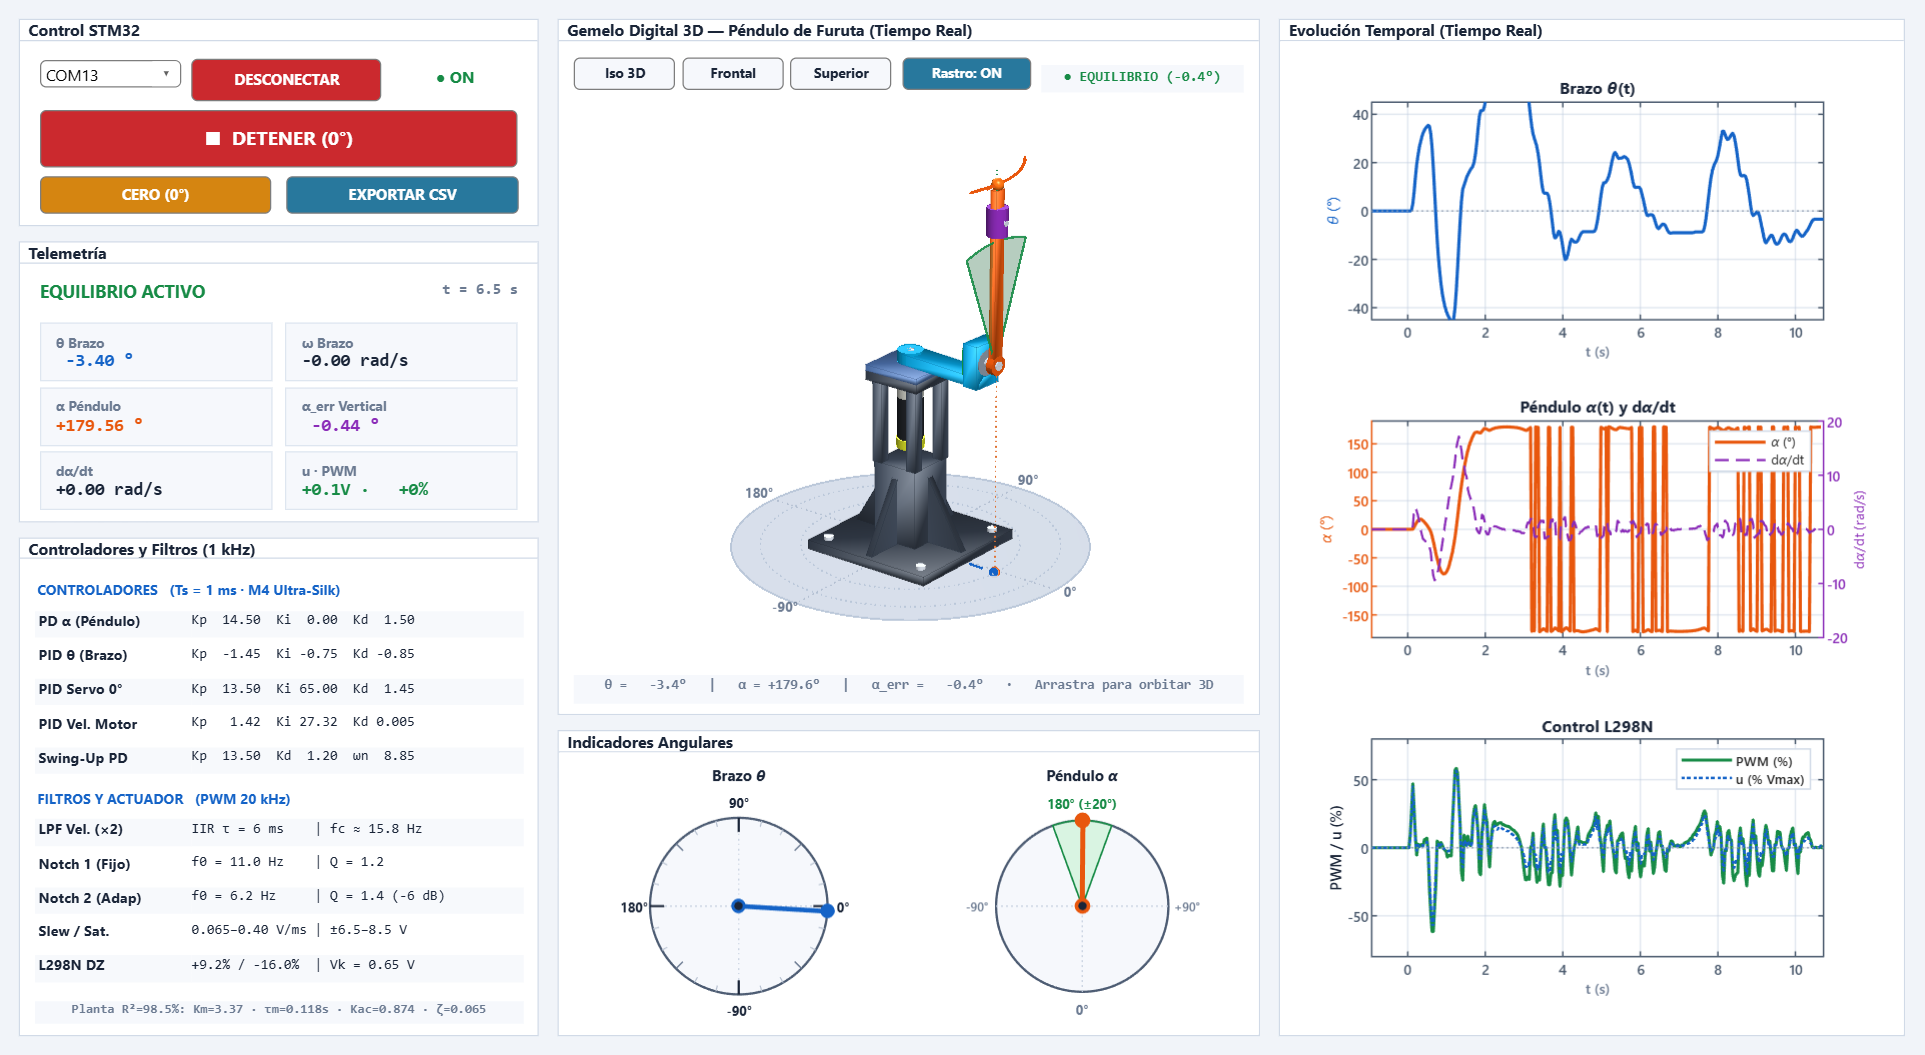
\includegraphics[width=0.66\textwidth]{fig_interfaz_matlab_gui.png}
    \caption{Interfaz gráfica de telemetría y gemelo digital 3D en MATLAB.}
    \label{fig:interfaz_matlab}
\end{figure*}

\textit{(i)~Necesidad:} supervisar en vivo estados internos rápidos no apreciables visualmente ($\tilde{\alpha}$, $\dot{\alpha}$, esfuerzo $u$ frente a PWM y transiciones de la FSM), comandar el sistema de forma ergonómica y almacenar trazas experimentales CSV reproducibles.
\textit{(ii)~Elección:} frente a monitores seriales de texto o gráficas 2D aisladas, un gemelo digital~3D estructurado mediante nodos jerárquicos \texttt{hgtransform} en MATLAB actualiza la cinemática espacial mediante transformaciones matriciales rígidas $\mathcal{O}(1)$ sin reconstruir polígonos ni bloquear la recepción serial.
\textit{(iii)~Diseño e (iv)~Implementación:} programada en \texttt{interfaz\_matlab/app\_telemetria\_sistema\_\allowbreak furuta\_matlab.m} (Fig.~\ref{fig:interfaz_matlab}), la aplicación adopta una distribución en tres columnas sincronizada con el puerto \texttt{COM13} a \qty{115200}{\baud} (terminador \texttt{CR/LF}):
\begin{itemize}
    \item \textbf{Columna~1 (Control, telemetría y constantes):} gestiona la conexión serial (\texttt{COM13}), el botón maestro único \texttt{Iniciar/Detener} (despacha ráfaga idempotente \texttt{START} o parada ordenada \texttt{STOPHOME}), el calibrador \texttt{Cero (0°)} (\texttt{ZERO}), el registro en disco \texttt{Exportar CSV} (matriz de 9 columnas), seis mosaicos KPI numéricos en tiempo real ($\theta$, $\omega$, $\alpha$, $\alpha_{\text{err}}$, $\dot{\alpha}$, así como tensión $u$ y ciclo útil PWM) junto con el estado FSM y reloj, y la tabla resumen de constantes activas \texttt{M4 Ultra-Silk}.
    \item \textbf{Columna~2 (Gemelo digital 3D y diales polares):} anima a \qty{30}{\hertz} el modelo tridimensional con cotas reales ($Z_{\text{piv}}=\qty{182.8}{\milli\meter}$, distancia pivote--punta \qty{152.8}{\milli\meter}) usando el nodo padre \texttt{T\_arm} (\texttt{zrotate} de $\theta$) y el nodo hijo \texttt{T\_pend} (\texttt{translate} al pivote más \texttt{xrotate} de $\alpha$), con selectores de cámara (\texttt{Iso 3D}, \texttt{Frontal}, \texttt{Superior}), rastro tridimensional de 90 puntos de la punta con proyección vertical al plano mesa, cono translúcido de captura ($\pm\qty{20}{\degree}$) y dos diales polares 2D sincronizados para $\theta$ y $\alpha$.
    \item \textbf{Columna~3 (Series temporales en vivo):} representa tres ventanas deslizantes sincronizadas de $400$ muestras para la posición del brazo $\theta(t)$, la deflexión pendular $\alpha(t)$ superpuesta con su velocidad $\dot{\alpha}(t)$ en doble eje vertical, y la comparación simultánea entre el esfuerzo solicitado $u(t)$ normalizado y el ciclo útil $\mathrm{PWM}(\%)$ efectivo entregado al L298N.
\end{itemize}

\subsection{Simulador Interactivo 3D de Cinemática Matricial y Repositorio de Reproducibilidad}\label{subsec:simulador_cinematica}

\begin{figure*}[!t]
    \centering
    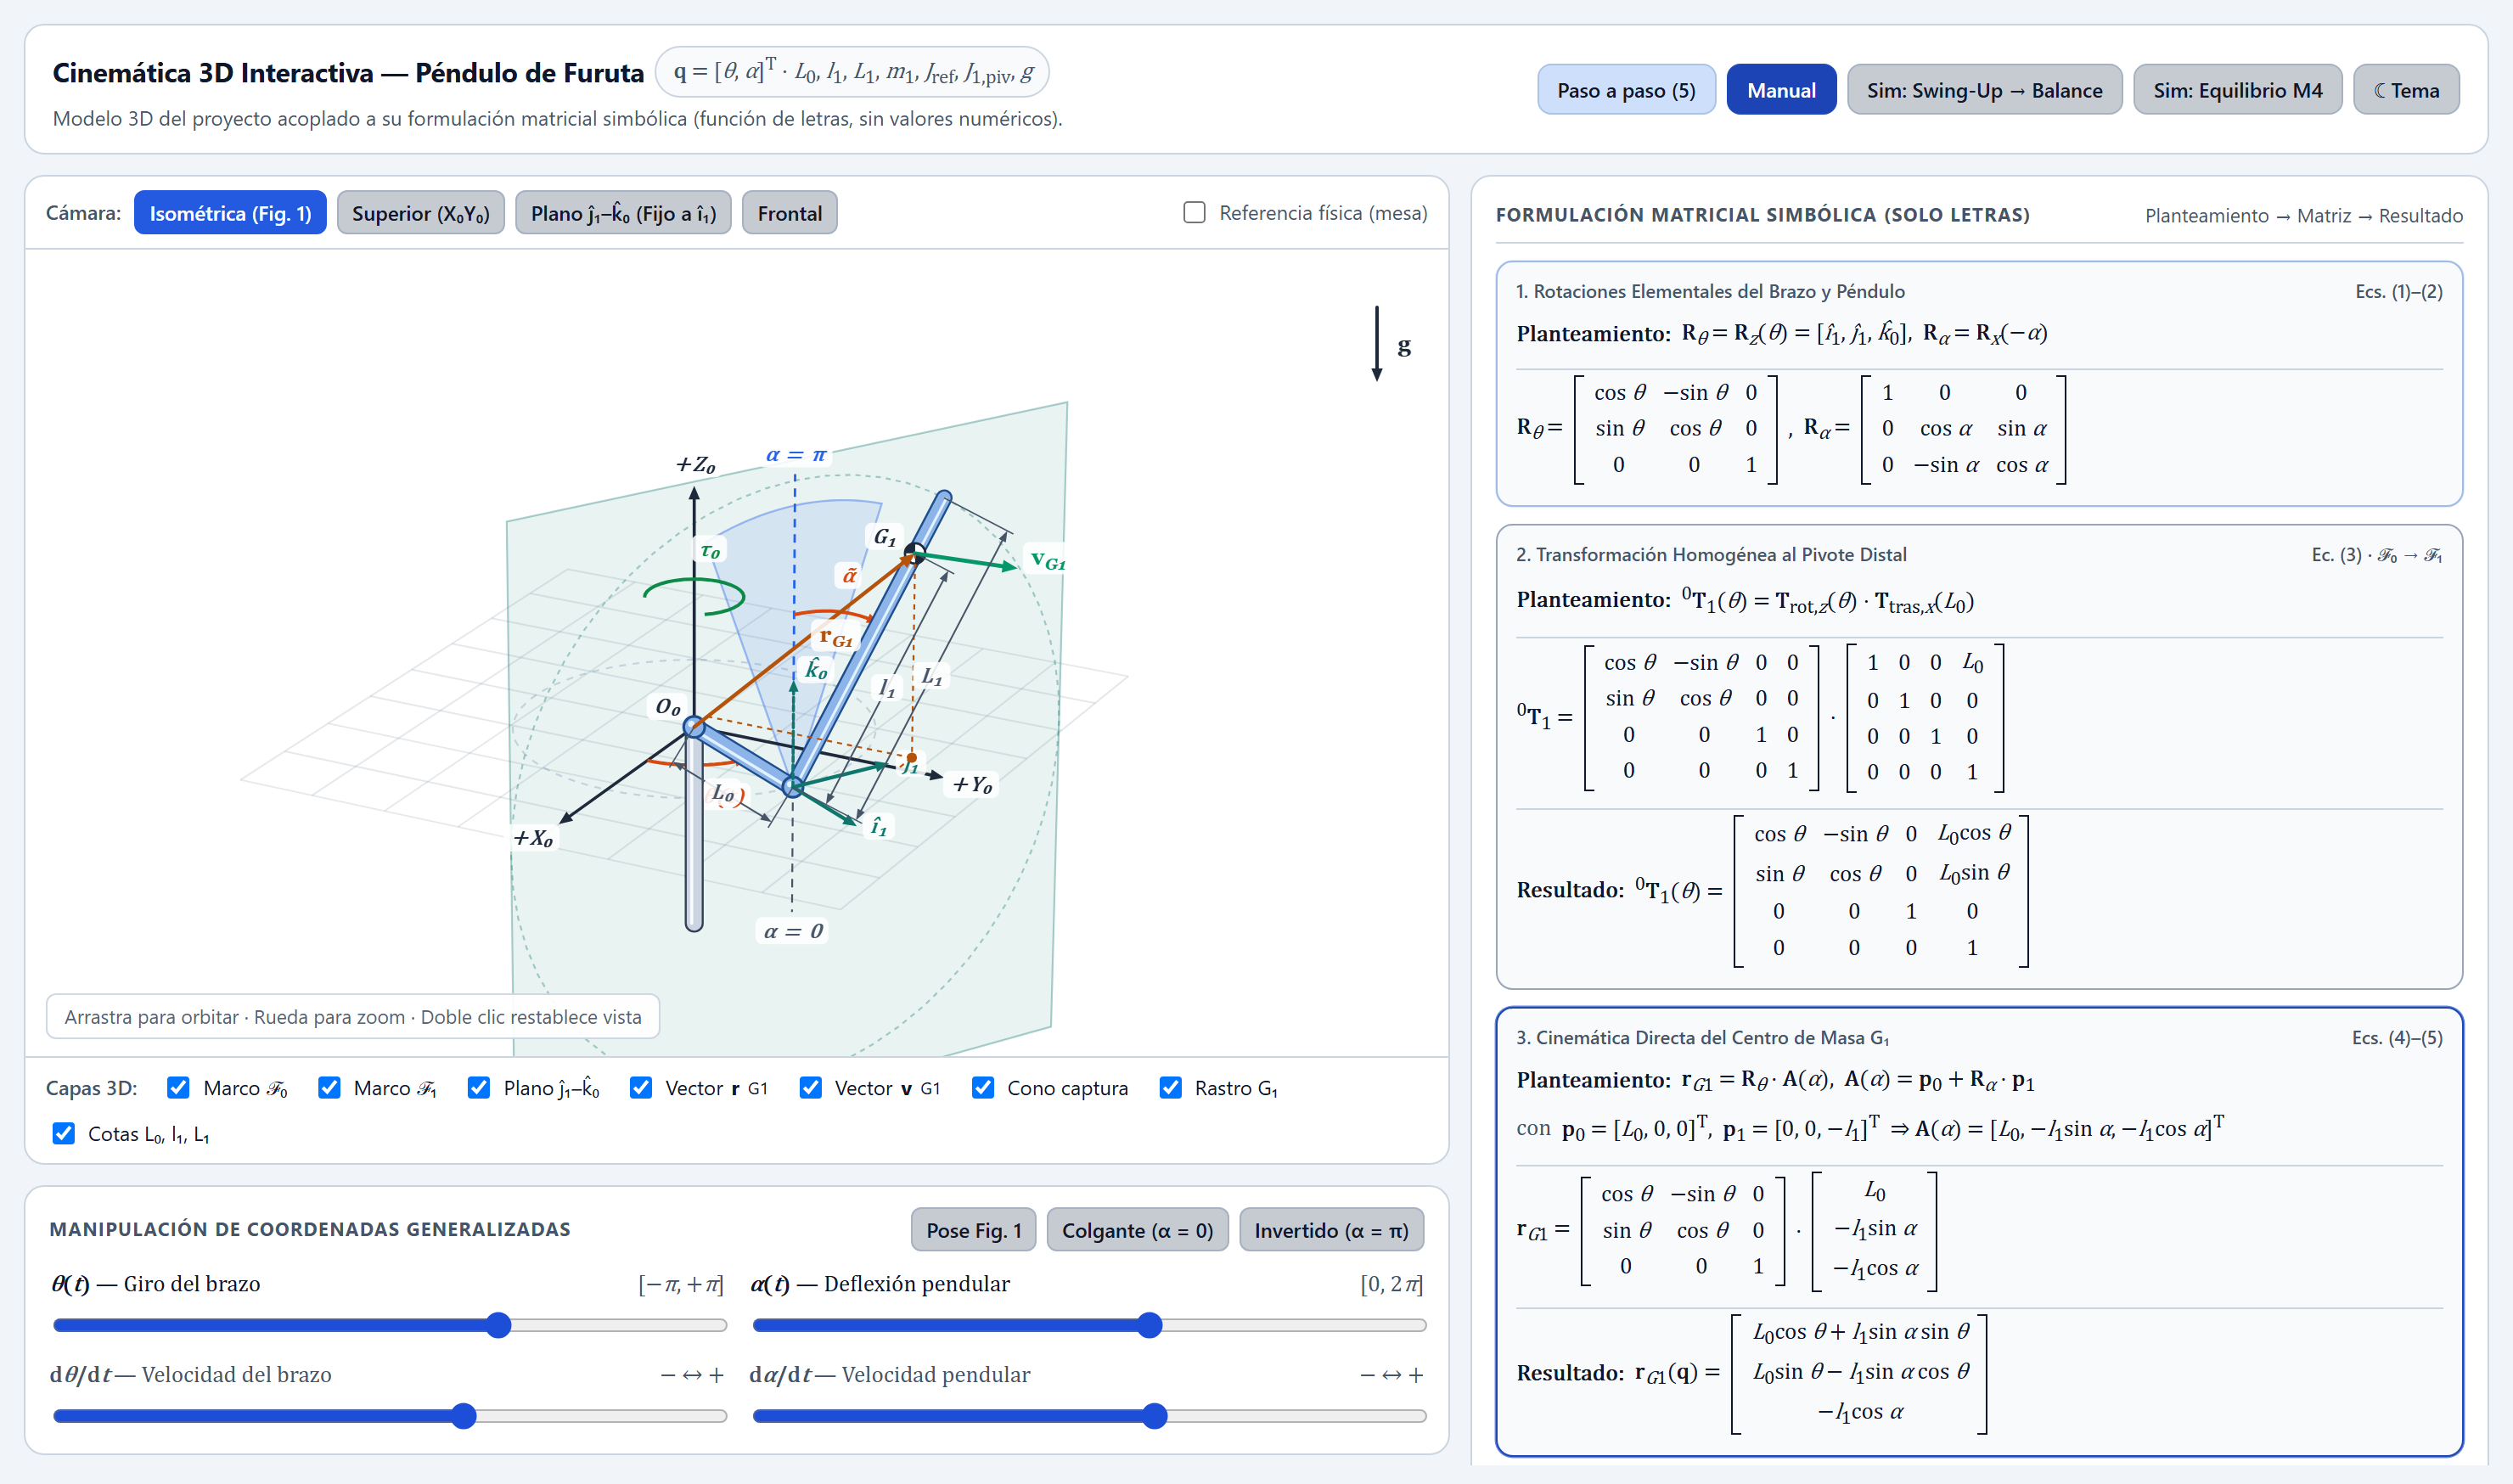
\includegraphics[width=0.70\textwidth]{fig_simulador_cinematica_3d.png}
    \caption{Simulador interactivo 3D de la cinemática matricial simbólica.}
    \label{fig:simulador_cinematica_3d}
\end{figure*}

\textit{(i)~Necesidad:} mientras el gemelo digital en MATLAB se orienta a la supervisión en vivo de la planta física vía \texttt{COM13}, el estudio y verificación didáctica del modelado cinemático tridimensional~\eqref{eq:marco_movil}--\eqref{eq:dinamica_alpha} requiere inspeccionar libremente cada rotación elemental, el plano móvil de oscilación y los vectores de posición y velocidad sin depender de licencias de software ni del hardware conectado.
\textit{(ii)~Elección:} se diseñó una aplicación web autónoma en un único archivo ejecutable fuera de línea (\textit{standalone} HTML5 Canvas, CSS y JavaScript puro, sin librerías ni dependencias externas), garantizando portabilidad inmediata en cualquier navegador moderno directamente desde el repositorio oficial del proyecto.
\textit{(iii)~Diseño:} como se observa en la Fig.~\ref{fig:simulador_cinematica_3d}, la interfaz divide la pantalla en un motor gráfico~3D interactivo a \qty{60}{\hertz} con cámara orbital, acercamiento por rueda y cuatro vistas preestablecidas (isométrica equivalente a la Fig.~\ref{fig:cinematica_furuta}, superior sobre el plano horizontal, vista fijada al plano móvil de oscilación y frontal) junto a un panel sincronizado de cinco tarjetas matriciales puramente simbólicas que muestran el planteamiento, el producto matricial explícito y el resultado de~\eqref{eq:marco_movil}--\eqref{eq:dinamica_alpha}. El usuario puede alternar entre cuatro modos operativos: recorrido guiado en cinco pasos vinculados a cada bloque ecuacional, manipulación manual continua de las coordenadas y velocidades generalizadas ($\theta$, $\alpha$, $\dot{\theta}$ y $\dot{\alpha}$) con poses rápidas, simulación numérica RK4 en vivo de la transición autónoma \texttt{SWING\_UP} hacia \texttt{BALANCE\_PID} y estabilización \texttt{M4 Ultra-Silk} con inyección interactiva de perturbaciones impulsionales, además de conmutación de capas visuales ($\mathcal{F}_0$, $\mathcal{F}_1$, plano móvil, $\mathbf{r}_{G1}$, $\mathbf{v}_{G1}$, cono de captura, rastro del centro de masa, cotas y referencia física de la mesa) y selector de tema claro u oscuro.
\textit{(iv)~Implementación y repositorio:} el simulador reside en \texttt{simulacion cinematica/\allowbreak index.html} dentro del repositorio público \url{https://github.com/Nocudo/Pendulo-Furuta-Control-Digital}, el cual consolida de manera versionada el diseño CAD (\texttt{cad/}), las placas DfAM listas para laminar (\texttt{IMPRESION\_3D/}), el firmware embebido STM32 (\texttt{firmware\_stm32/}), los registros experimentales y análisis (\texttt{caracterizacion\_\allowbreak y\_\allowbreak validacion/}), la interfaz MATLAB (\texttt{interfaz\_matlab/}), la documentación técnica (\texttt{docs/}) y el presente artículo (\texttt{articulo/}).
